% Options for packages loaded elsewhere
\PassOptionsToPackage{unicode}{hyperref}
\PassOptionsToPackage{hyphens}{url}
% !TeX program = pdfLaTeX
\documentclass[12pt]{article}
\usepackage{amsmath}
\usepackage{graphicx,psfrag,epsf}
\usepackage{enumerate}
\usepackage[]{natbib}
\usepackage{textcomp}


%\pdfminorversion=4
% NOTE: To produce blinded version, replace "0" with "1" below.
\newcommand{\blind}{0}

% DON'T change margins - should be 1 inch all around.
\addtolength{\oddsidemargin}{-.5in}%
\addtolength{\evensidemargin}{-1in}%
\addtolength{\textwidth}{1in}%
\addtolength{\textheight}{1.7in}%
\addtolength{\topmargin}{-1in}%

%% load any required packages here



% tightlist command for lists without linebreak
\providecommand{\tightlist}{%
  \setlength{\itemsep}{0pt}\setlength{\parskip}{0pt}}



\usepackage[dvipsnames]{xcolor} % colors
\newcommand{\ear}[1]{{\textcolor{blue}{#1}}}
\newcommand{\svp}[1]{{\textcolor{RedOrange}{#1}}}
\newcommand{\rh}[1]{{\textcolor{Green}{#1}}}
\newcommand\pcref[1]{(\cref{#1})}
\usepackage{algorithm,algpseudocode,booktabs}
\usepackage{hyperref}
\usepackage[capitalise]{cleveref}
\usepackage{xr} \externaldocument{appendix}
\usepackage{subfig}

\IfFileExists{bookmark.sty}{\usepackage{bookmark}}{\usepackage{hyperref}}
\IfFileExists{xurl.sty}{\usepackage{xurl}}{} % add URL line breaks if available
\hypersetup{
  pdftitle={Perception and Cognitive Implications of Logarithmic Scales for Exponentially Increasing Data: Perceptual Sensitivity Tested with Statistical Lineups},
  pdfkeywords={log scales, visual inference, graphical testing},
  hidelinks,
  pdfcreator={LaTeX via pandoc}}



\begin{document}


\def\spacingset#1{\renewcommand{\baselinestretch}%
{#1}\small\normalsize} \spacingset{1}


%%%%%%%%%%%%%%%%%%%%%%%%%%%%%%%%%%%%%%%%%%%%%%%%%%%%%%%%%%%%%%%%%%%%%%%%%%%%%%

\if0\blind
{
  \title{\bf Perception and Cognitive Implications of Logarithmic Scales
for Exponentially Increasing Data: Perceptual Sensitivity Tested with
Statistical Lineups}

  \author{
        Emily A. Robinson 1 \\
    Department of Statistics, California Polytechnic State University -
San Luis Obispo\\
     and \\     Reka Howard 2 \\
    Department of Statistics, University of Nebraska - Lincoln\\
     and \\     Susan VanderPlas 3 \\
    Department of Statistics, University of Nebraska - Lincoln\\
      }
  \maketitle
} \fi

\if1\blind
{
  \bigskip
  \bigskip
  \bigskip
  \begin{center}
    {\LARGE\bf Perception and Cognitive Implications of Logarithmic
Scales for Exponentially Increasing Data: Perceptual Sensitivity Tested
with Statistical Lineups}
  \end{center}
  \medskip
} \fi

\bigskip
\begin{abstract}
Logarithmic transformations are a standard solution to displaying data
that span several magnitudes within a single graph. This paper
investigates the impact of log scales on perceptual sensitivity through
a visual inference experiment using statistical lineups. Our study
evaluated participant's ability to detect differences between
exponentially increasing data, characterized by varying levels of
curvature, using both linear and logarithmic scales. Participants were
presented with a series of plots and asked to identify the panel that
appeared most different from the others. Due to the choice of scale
altering the contextual appearance of the data, the results revealed
slight perceptual advantages for both scales depending on the curvatures
of the compared data. This study serves as the initial part of a
three-paper series dedicated to understanding the perceptual and
cognitive implications of using logarithmic scales for visualizing
exponentially increasing data. These studies serve as an example of
multi-modal graphical testing, examining different levels of engagement
and interaction with graphics to establish nuanced and specific
guidelines for graphical design.
\end{abstract}

\noindent%
{\it Keywords:} log scales, visual inference, graphical testing

\vfill

\newpage
\spacingset{1.9} % DON'T change the spacing!

\section{Introduction}\label{introduction}

Effective communication of data is critical in influencing people's
opinions and actions. This consideration was particularly true during
the COVID-19 pandemic, where data visualizations and dashboards were
vital in informing the public and policymakers about the outbreak's
status. Local governments relied on graphics to inform their decisions
about shutdowns and mask mandates, while residents were presented with
data visualizations to encourage compliance with these regulations. A
major issue designers encountered when creating COVID-19 plots was how
to display data from a wide range of values
\citep{fagen-ulmschneider_2020, burnmurdoch_2020}. When faced with data
that span several orders of magnitude, we must decide whether to show
the data on its original scale - where smaller magnitudes are
compressed, making them harder to discern - or to transform the scale,
which alters the contextual appearance of the data. Logarithmic axis
transformations have emerged as a standard solution to this challenge,
as they allow for the display of data over several orders of magnitude
within a single graph.

Exponential data are one such example where, on a linear scale, the
separation of data at smaller magnitudes becomes difficult to discern;
\cref{fig:log-scales} presents hard drive capacity over the past forty
years on both the linear and log scales to demonstrate the usefulness of
log scales when dealing with data spanning multiple magnitudes.
Logarithms facilitate the conversion of multiplicative relationships
(where the apparent distance between numbers like 1 \& 10 or 10 \& 100
grows multiplicatively) to additive relationships (displaying these same
intervals as equal distances), highlighting proportional relationships
and linearizing power functions \citep{menge_logarithmic_2018}.
Logarithms also have practical applications, simplifying the computation
of small numbers such as likelihoods and transforming data to conform to
statistical assumptions. Although log scales have a long history of use
in fields such as ecology, psychophysics, engineering, and physics
\citep{heckler_student_2013, waddell2005comparisons}, there is still a
need to understand the implications of their use and provide best
practices for their implementation.

\begin{figure}[tbp]

{\centering 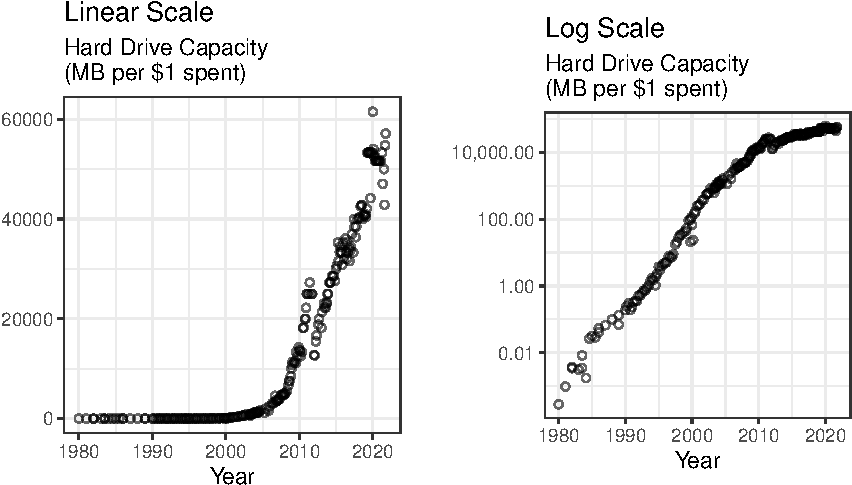
\includegraphics[width=1\linewidth,]{logarithmic-lineups-revisions-3_files/figure-latex/log-scales-1} 

}

\caption{These plots present hard drive capacity \citep{memdisk} over the past forty years on both the linear and log scale and illustrate the use of the log scale when displaying data which spans several magnitudes.}\label{fig:log-scales}
\end{figure}

Apart from the biases resulting from using log scales, there is a
general misinterpretation of exponential growth. Previous studies have
explored the estimation and prediction of exponential growth and found
that individuals often underestimate exponential growth when presented
values numerically and graphically
\citep{wagenaar_misperception_1975, ciccione2022analyzing}. The
hierarchy of plot objects, such as lengths and angles, as described by
\citet{cleveland_graphical_1985}, offers a possible explanation for the
underestimation observed in exponentially increasing trends. Experiments
conducted by \citet{wagenaar_misperception_1975},
\citet{jones_polynomial_1977}, and \citet{mackinnon_feedback_1991} aimed
to improve estimation accuracy for exponential growth. While contextual
knowledge or experience did not enhance estimation, instruction on
exponential growth reduced underestimation by prompting participants to
adjust their initial starting value
\citep{wagenaar_misperception_1975, jones_polynomial_1977}. Furthermore,
providing immediate feedback to participants about the accuracy of their
predictions improved estimation \citep{mackinnon_feedback_1991}.
Recently, \citet{lammers2020correcting} found that people misperceived
exponential growth as increasing linearly, and that providing
instructions to individuals about the exponential growth reduced this
misperception. These misinterpretations and misperceptions can lead to
decisions made under inaccurate understanding, resulting in potential
consequences.

Log transforming the data may address our inability to predict
exponential growth accurately. However, this transformation introduces
new complexities, as most readers may need to be mathematically
sophisticated enough to intuitively understand logarithmic math and
translate it back into real-world effects. Despite the transformative
power of logarithmic scales in facilitating accurate data
representation, \citet{menge_logarithmic_2018}'s survey of ecologists
highlights the challenges associated with the widespread comprehension
of log-scaled data. Notably, the study identifies prevalent
misconceptions arising from linear extrapolation assumptions in log-log
space, a factor that often leads to neglect of the underlying
exponential relationships in linear-linear space.

Building upon the need for a nuanced understanding of data
representation, \citet{buja_statistical_2009} introduced statistical
lineups as a framework for statistical inference and graphical tests.
Statistical lineups treat a data plot as a visual statistic, summarizing
the data as a numerical function or mapping. Evaluation of a panel in a
statistical lineup requires visual inspection by a person, and if visual
evaluations lead to different results, two visualization methods are
deemed significantly different. Recent studies have utilized statistical
lineups to quantify the perception of graphical design choices
\citep{hofmann_graphical_2012, loy_model_2017, loy_variations_2016, vanderplas_clusters_2017}.
Statistical lineups provide an elegant way of combining perception and
statistical hypothesis testing through graphical experiments
\citep{majumder_validation_2013, vanderplas_testing_2020, wickham2010graphical}.

The term `lineup' is an analogy to police lineups in criminal
investigations, where witnesses identify the criminal from a group of
individuals. Similarly, researchers present a statistical lineup plot
consisting of smaller panels and ask the viewer to identify the panel
that contains the actual data from a set of decoy null plots.
Researchers generate null plots containing data generated according to a
prespecified hypothesis using permutation or simulation. Typically, a
statistical lineup consists of 20 panels, with one target panel and 19
null panels. If the viewer can identify the target panel from the null
panels, it suggests that the actual data is visually distinct from the
data generated under the null model.

While explicit graphical tests direct the participant to a specific
feature of a plot to answer a particular question, implicit graphical
tests require the user to identify both the purpose and function of the
plot in order to evaluate the plots shown. Furthermore, implicit
graphical tests, such as lineups, simultaneously test for multiple
visual features, including outliers, clusters, and linear and nonlinear
relationships \citep{vanderplas2015spatial}. Researchers can collect
responses from multiple viewers using crowd-sourcing websites such as
Prolific and Amazon Mechanical Turk.

In this paper, our primary focus is to evaluate the perceptual
sensitivity towards the degree of curvature as a result of displaying
data on linear and log scales. To address this, we conducted a visual
inference experiment employing statistical lineups
\citep{buja_statistical_2009}. Although our findings could have broad
applications to various functions resulting in curvature, our experiment
deliberately centered on participants' ability to identify differences
in the curvature of exponentially increasing curves when presented on
differing scales, thus altering their curvature appearance. We discuss
the nuances and challenges of testing the perception of exponential
growth in the appendix. Importantly, this investigation did not
necessitate participants to undergo mathematical training or possess a
prior understanding of exponential growth or logarithmic scales.
Instead, it aimed to unravel the inherent ability to identify
differences in curvature within charts, focusing on the fundamental
nature of visual perception.

In \hyperref[methods]{Section 2} we describe the participant sample, the
graphical task, data generation process, and study design.
\hyperref[results]{Section 3} describes the participant data collected
and shares results from the statistical analyses of the data using a
generalized linear mixed model. We present overall conclusions and
discussion of the results in \hyperref[conclusion-discussion]{Section
4}, and provide an overview of future related papers. The
\hyperref[supplementary-material]{Supplementary Material} includes a
link to the RShiny data collection applet, participant data used for
analysis, and code to replicate the analysis. The results of this study
lay the groundwork for further exploration of the implications of using
log scales in data visualization.

\section{Study Development and Methods}\label{methods}

\subsection{Data Generation}\label{data-generation}

In this study, we simulated data from a two-parameter exponential
function with a vertical shift to generate the target and null data
sets; the curve equations between panels differ in the parameter values
selected for the null and target panels. In order to guarantee the
simulated data spans the same domain and range of values for each
statistical lineup panel, we began with a domain constraint of
\(x\in [0,20]\) and a range constraint of \(y\in [10,100]\) with
\(N = 50\) points randomly assigned throughout the domain. We mapped the
randomly generated \(x\) values to a corresponding \(y\) value based on
the function curve with predetermined parameter values and
multiplicative random errors to simulate the response. Finally, we
applied a vertical shift constraint. These constraints assure that
participants who select the target panel are doing so because of their
visual perception differentiating between curvature or growth rate
rather than different starting or ending values.

We simulated data based on a two-parameter exponential function extended
with an additional parameter for multiplicative errors and a vertical
shift, for a total of four parameters:

\begin{align}
y_i & = \alpha\cdot e^{\beta\cdot x_i + \epsilon_i} + \theta \\
\text{with } \epsilon_i & \sim N(0, \sigma^2) \nonumber
\end{align}

where \(\alpha\) controls the vertical extent, \(\beta\) affects the
rate of growth, and \(\theta\) provides a vertical shift of the
function. The parameters \(\alpha\) and \(\theta\) were necessary to
adjust based on \(\beta\) and \(\sigma^2\) to guarantee the range and
domain constraints are met. It is worth noting that while the inclusion
of \(\theta\) allows for constraints on the range, when a log
transformation is applied, the curve loses the linearity properties
typically seen with log transformed exponential data.

Equation (1) was used to generate \(N = 50\) points
\((x_i, y_i), i = 1,...,N\) where \(x\) and \(y\) have an increasing
exponential relationship. We selected parameters and generated data
using a heuristic approach rather than algebraic to ensure the parameter
selections resulted in visually distinct curves.

In summary, we identified three points (start, midpoint, and end) we
wanted the curve to pass through. These control the level of curvature
seen in the data. Then we optimized a nonlinear least squares regression
line using the function from Equation (1) to obtain parameters used for
simulating the data sets with multiplicative errors and a vertical
shift. We provide details for the heuristic data generation procedure in
\cref{alg:lineup-parameter-estimation-algorithm} and
\cref{alg:lineup-exponential-data-simulation-algorithm}.

\begin{algorithm}
  \caption{Lineup Parameter Estimation}\label{alg:lineup-parameter-estimation-algorithm}
  \begin{algorithmic}[1]
    \Statex \hspace*{-1em}\textbullet~\textbf{Input Parameters:} domain $x\in[0,20]$, range $y\in[10,100]$, midpoint $x_{mid}$.
    \Statex \hspace*{-1em}\textbullet~\textbf{Output Parameters:} estimated model parameters $\hat\alpha, \hat\beta, \hat\theta$.
    \State In order to estimate three parameters, we jittered two $x$ values around the pre-selected midpoint (depends on curvature) for a total of four points ($x_{min}$, $x_{mid}-1$, $x_{mid}+1$, $x_{max}$)
    \State The starting and ending $x$ values correspond to $y$ values from the predefined range providing two points, $(0,0)$ and $(20,100)$
    \State To determine the $y$ value corresponding to the midpoints, we first computed the point-slope form of the line passing through $(0,100)$ and $(20,0)$, resulting in $y=-5\cdot x+100$. Perceptually, when plotting with an aspect ratio of 1, this appears as a line with a $-45^{\circ}$ angle, similar to what we typically see in a $y=-x$ line, although algebraically it is scaled to fit the assigned domain and range.
    \State Next, we determined the $y$ value associated with the two additional middle points, $x_{mid} - 0.1$ and $x_{mid} + 0.1$, using the equation of the line determined in (3). This provides us our four points for estimating the three parameters.
    \State From the set of points $(x_k, y_k)$ for $k = 1,2,3,4$, calculate the coefficients from the linear regression model $\ln(y_k) = b_0 +b_1x_k$ to obtain starting values for $\alpha_0 = e^{b_0}, \beta_0 =  b_1, \theta_0 = 0.5\cdot \min(y)$
    \State Using the \texttt{nls} function from the base \texttt{stats} package in Rstudio \citep{Rstudio} and the starting parameter values - $\alpha_0, \beta_0, \theta_0$ - fit the nonlinear model, $y_k = \alpha\cdot e^{\beta\cdot x_k}+\theta$ to get estimated parameter values for $\hat\alpha, \hat\beta, \hat\theta.$
  \end{algorithmic}
\end{algorithm}

\begin{algorithm}
  \caption{Lineup Exponential Data Simulation}\label{alg:lineup-exponential-data-simulation-algorithm}
  \begin{algorithmic}[1]
    \Statex \hspace*{-1em}\textbullet~\textbf{Input Parameters:} sample size $N = 50$, estimated parameters $\hat\alpha$, $\hat\beta$, and $\hat\theta$, from \cref{alg:lineup-parameter-estimation-algorithm}, and standard deviation $\sigma$ from the exponential curve.
    \Statex \hspace*{-1em}\textbullet~\textbf{Output Parameters:} $N$ points, in the form of vectors $\mathbf{x}$ and $\mathbf{y}$.
    \State Generate $\tilde x_j, j = 1,..., \frac{3}{4}N$ as a sequence of evenly spaced points in $[0,20]$. This ensures the full domain of $x$ is used, fulfilling the constraints of spanning the same domain and range for each parameter combination.
    \State Obtain $\tilde x_i, i = 1,...,N$ by sampling $N = 50$ values from the set of $\tilde x_j$ values. This guarantees some variability and potential clustering in the exponential growth curve disrupting the perception due to continuity of points.
    \State Obtain the final $x_i$ values by jittering $\tilde x_i$.
    \State Calculate $\tilde\alpha = \frac{\hat\alpha}{e^{\sigma^2/2}}.$ This ensures that the range of simulated values for different standard deviation parameters has an equal expected value for a given rate of change due to the non-constant variance across the domain.
    \State Generate $y_i = \tilde\alpha\cdot e^{\hat\beta x_i + e_i}+\hat\theta$ where $e_i\sim N(0,\sigma^2).$
  \end{algorithmic}
\end{algorithm}

\subsection{Parameter Selection}\label{lineups-parameter-selection}

We chose three levels of trend curvature (low curvature, medium
curvature, and high curvature). For each curvature level, we simulated
1,000 data sets of \((x_{ij}, y_{ij})\) points for \(i = 1,...,50\)
increments of \(x\)-values and replicated \(j = 1,...,10\) corresponding
\(y\)-values per \(x\)-value. Each generated \(x_i\) point from
\cref{alg:lineup-exponential-data-simulation-algorithm} was replicated
ten times. Using the \texttt{lm} function from base R, we fit a linear
regression model on each of the individual data sets and included the
explanatory variable as both numeric and categorical. We then computed
the lack of fit statistic (LOF) which measures the deviation of the data
from the linear regression model \citep{Kutner_2004, Stroup_2013} using
the \texttt{anova} function from base R to determine the F-test effect
of the categorical explanatory variable. After obtaining the LOF
statistic for each level of curvature, we evaluated the density plots
(\cref{fig:lof-density-curves}) to provide a metric for differentiating
between the curvature levels and thus detecting the target plot. While
the LOF statistic provides a numerical value for discriminating between
the difficulty levels, it cannot be directly related to the perceptual
discriminability; it serves primarily as an approximation to ensure that
we are testing parameters at several distinct curvature levels.
\cref{tab:parameter-data} lists the final parameters used for data
simulation.

\begin{figure}[tbp]

{\centering 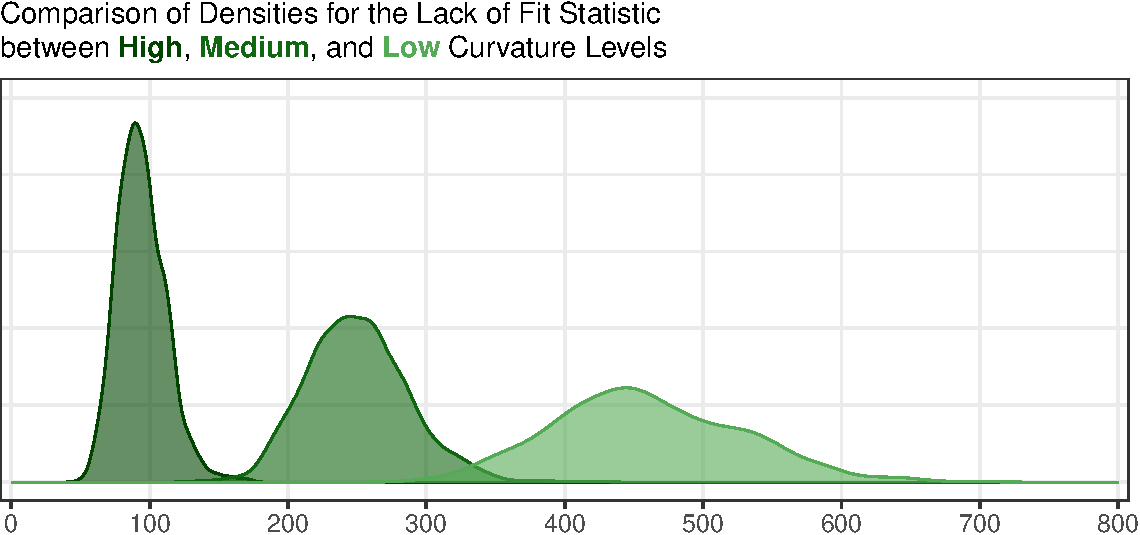
\includegraphics[width=1\linewidth,]{logarithmic-lineups-revisions-3_files/figure-latex/lof-density-curves-1} 

}

\caption{Density plot of the lack of fit statistic showing separation of difficulty levels: obvious curvature, noticable curvature, and almost linear.}\label{fig:lof-density-curves}
\end{figure}

\begin{table}

\caption{\label{tab:parameter-data}Lineup data simulation final parameters}
\centering
\begin{tabular}[t]{lrrrrrr}
\toprule
Curvature Level & $x_{mid}$ & $\hat\alpha$ & $\tilde\alpha$ & $\hat\beta$ & $\hat\theta$ & $\hat\sigma$\\
\midrule
High & 14.5 & 0.91 & 0.88 & 0.23 & 9.10 & 0.25\\
Medium & 13.0 & 6.86 & 6.82 & 0.13 & 3.14 & 0.12\\
Low & 11.5 & 37.26 & 37.22 & 0.06 & -27.26 & 0.05\\
\bottomrule
\end{tabular}
\end{table}

\subsection{Lineup Setup}\label{lineup-setup}

To generate the small multiple scatter plots for the statistical lineups
shown to participants in the study, we simulated a single data set
corresponding to curvature level A for the target plot and multiple data
sets corresponding to curvature level B for the null plots. The
\texttt{nullabor} package in R \citep{buja_statistical_2009} randomly
assigned the target plot to one of the panels surrounded by panels
containing null plots. The target and null panels span a similar domain
and range due to the implemented constraints when simulating the data;
the rationale for this decision is based on preattentive feature
perception \citep{wolfeWhatPreattentiveFeature2019} and is discussed in
detail in the appendix. There were a total of six lineup curvature
combinations; \cref{fig:curvature-combination-example} illustrates the
six lineup curvature combinations (top: linear scale; bottom: log scale)
where the solid line indicates the curvature level designated to the
target plot while the dashed line indicates the curvature level assigned
to the null plots. Two sets of each lineup curvature combination were
simulated (a total of twelve test data sets) and plotted on both the
linear scale and the log scale (24 test lineup plots). In addition to
the experimental lineups, we generated two sets of homogeneous
``Rorschach'' lineups, each featuring panels simulated from the same
distribution for each of the three curvatures (a total of six Rorschach
data sets). Importantly, participants were unaware that there was no
designated target panel for identification. Each participant evaluated
one ``Rorschach'' lineup.

\begin{figure}[tbp]

{\centering 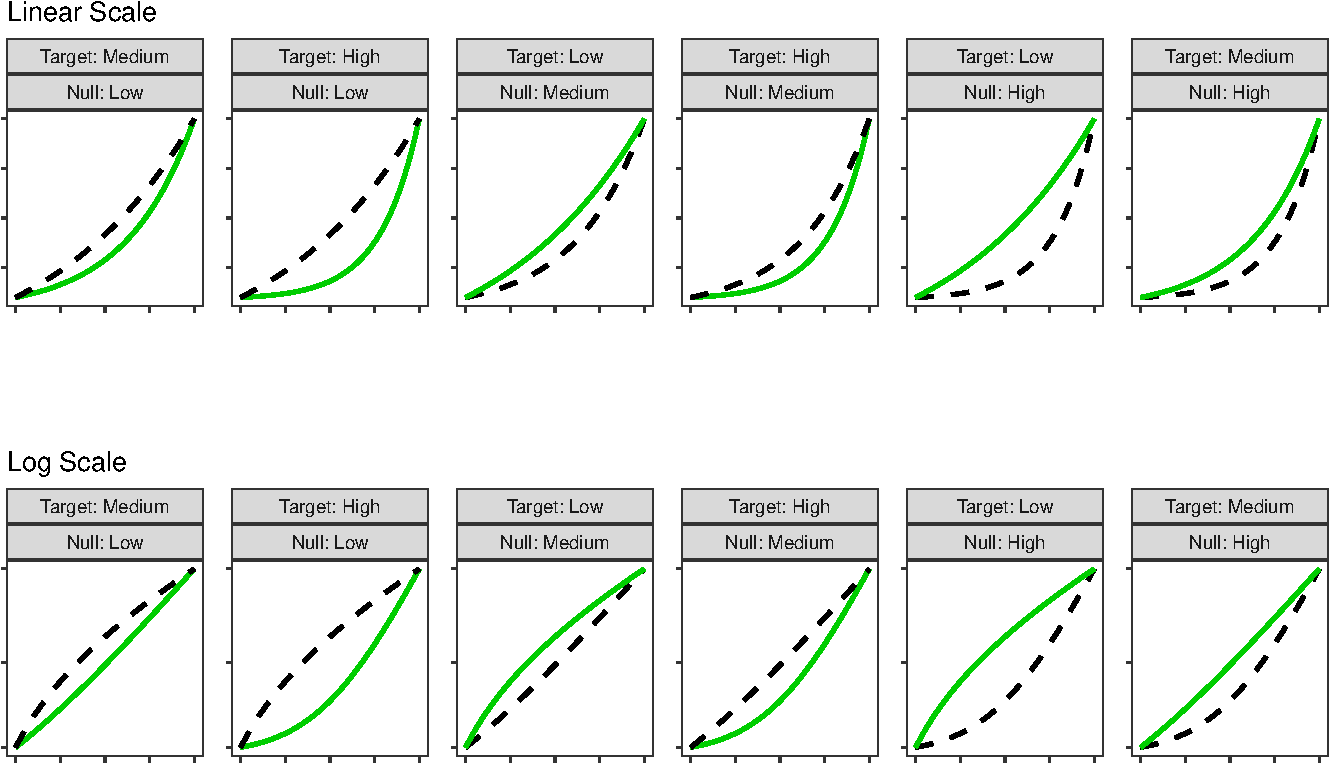
\includegraphics[width=1\linewidth,]{logarithmic-lineups-revisions-3_files/figure-latex/curvature-combination-example-1} 

}

\caption{Thumbnail plots illustrating the six curvature combinations displayed on both scales (linear and log). The solid line indicates the curvature level to be identified as the target plot from amongst a set of null plots with the curvature level indicated by the dashed line.}\label{fig:curvature-combination-example}
\end{figure}

\cref{fig:lineup-example} presents examples of statistical lineups with
the target data simulated with exponential parameters corresponding to
high curvature and the surrounding null panels simulated with parameters
for low curvature. The statistical lineup on the left presents
increasing exponential data displayed on a linear scale with panel 13 as
the target panel. The lineup on the right shows increasing exponential
data plotted on a log scale with panel 4 as the target panel.

\begin{figure}[tbp]

{\centering 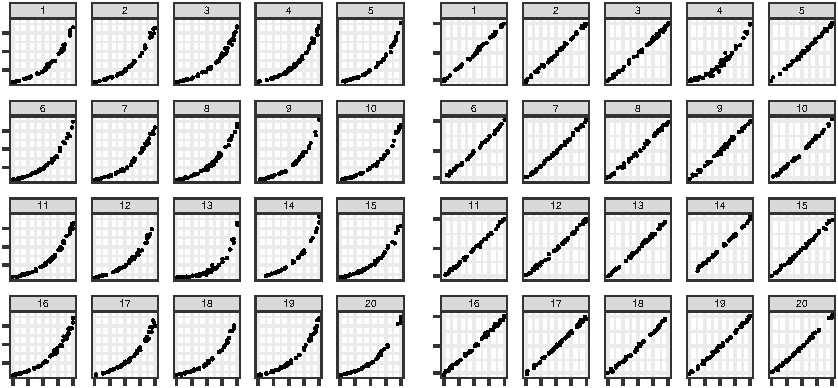
\includegraphics[width=\linewidth,]{logarithmic-lineups-revisions-3_files/figure-latex/lineup-example-1} 

}

\caption{The lineup plot on the left displays increasing exponential data on a linear scale with panel 13 as the target. The lineup plot on the right displays increasing exponential data on the log scale with panel 4 as the target.}\label{fig:lineup-example}
\end{figure}

\subsection{Study Design and
Implementation}\label{study-design-and-implementation}

We used Prolific, a survey site that connects researchers to study
participants, to recruit participants above the age of majority (18+ in
most regions; 19+ in NE and AL; 21+ in MS) in their region. We did not
request a representative sample, as previous literature indicates the
presence of only minor effects of demographics on the outcome of
graphical experiments involving lineups
\citep{vanderplas2015spatial, majumder_validation_2013}. Following the
completion of the current statistical lineup study, participants
sequentially completed two additional graphical experiments related to
the perception of logarithmic scales (to be discussed at a later date),
and we compensated them for their participation in the series of all
three studies.

We showed each participant 13 lineup plots (12 test and one Rorschach).
At the start of the study, we randomly assigned participants to one of
the two replicate data sets for each of the six unique lineup curvature
combinations. Participants evaluated the lineup plot corresponding to
the linear and log scales for each assigned test data set. For the
additional Rorschach lineup plot, we randomly assigned participants to
one data set shown on either the linear or the log scale. We randomized
the order in which participants saw the assigned 13 lineup plots.

\cref{fig:study-homepage} presents a screenshot of the study homepage,
which served as an introduction to participants and guided them through
the series of three graphical experiments. The first experiment,
discussed in this paper, utilized statistical lineups to investigate the
effect of logarithmic scales on perceptual sensitivity. The second
experiment incorporated an interactive `You Draw It' feature introduced
by \citet{aisch2015you} and employed in the study by
\citet{robinson2022eye}, to examine the effect of logarithmic scales on
prediction. The third experiment focused on numerical estimation and
cognitive understanding of logarithmic scales.

Participants completed the series of graphical tests using an R Shiny
application \citep{shiny_pkg} accessible at
\url{https://emily-robinson.shinyapps.io/perception-of-statistical-graphics-log/}.
The code used to implement the described methods for generating the
data, setting up the lineups, and implementing the study design is
available on GitHub at
\url{https://github.com/earobinson95/perception-of-statistical-graphics-log}.
Before completing the lineup study, the `You Draw It' study, and the
estimation study, participants were prompted to provide their
demographic information. The series of studies received an IRB exemption
(IRB \#20200720178EX) from the University of Nebraska - Lincoln.

\begin{figure}[tbp]

{\centering 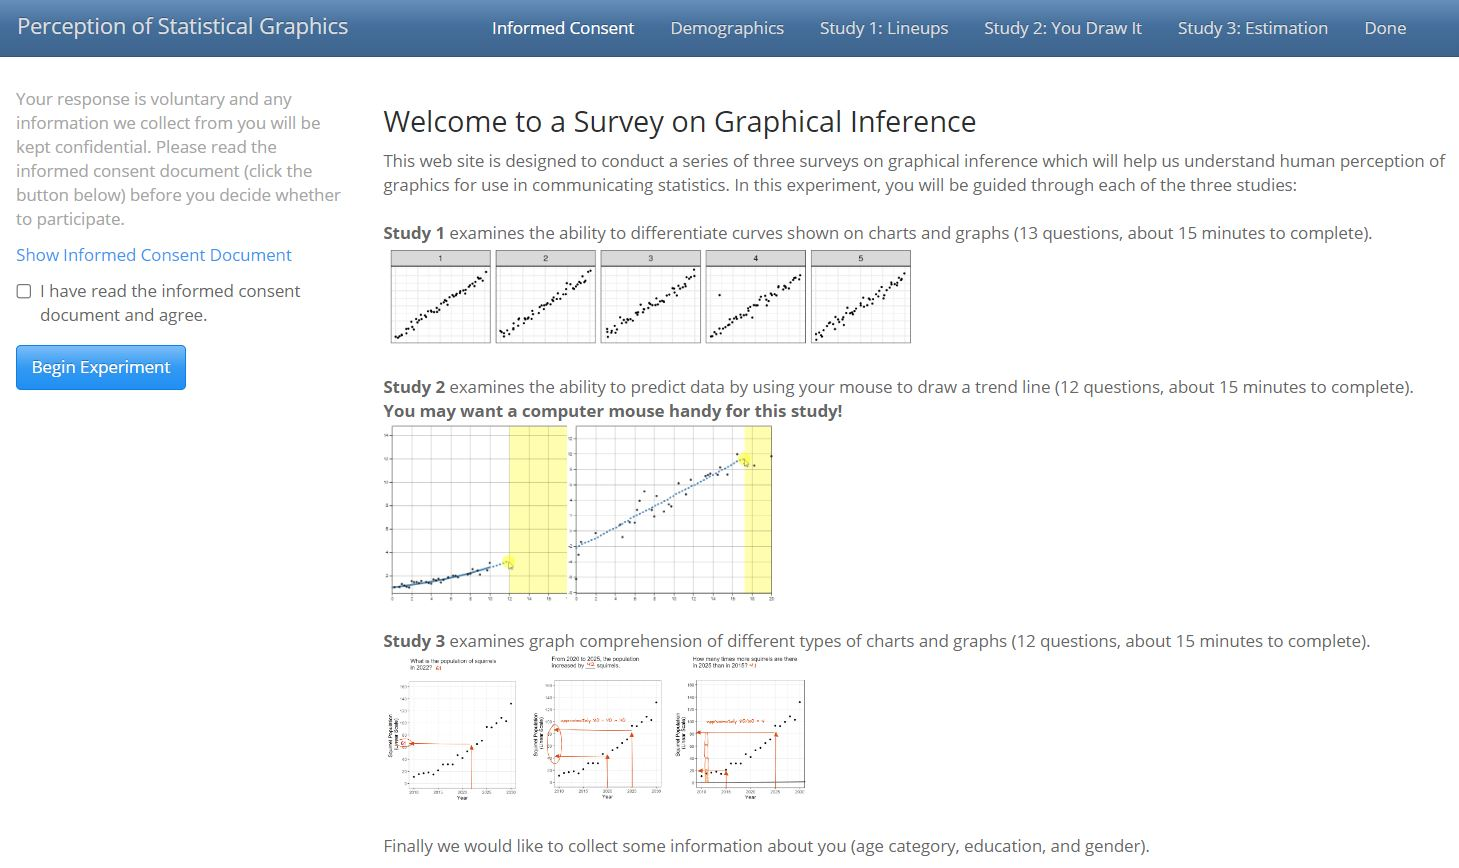
\includegraphics[width=1\linewidth,]{images/study-homepage} 

}

\caption{Screenshot of the study applet homepage guiding participants through the series of three graphical experiments related to the perception of logarithmic scales.}\label{fig:study-homepage}
\end{figure}

The statistical lineup study guided participants through the series of
13 lineup plots and asked them a single question per lineup, ``Which
plot is the most different?'' (\cref{fig:lineup-study-example-trial}).
In each lineup evaluation, participants then justified their choice in a
select all that apply format (Clustering, Different range, Different
shape, Outlier(s), and Other) under the ``Reasoning'' sidebar panel.
Additionally, participants provided their level of confidence in their
choice by answering ``How certain are you?'' on a five-point Likert
scale from very certain to very uncertain. This graphical task aimed to
test an individual's ability to perceptually differentiate exponentially
increasing trends with differing levels of curvature on both the linear
and log scales.

\begin{figure}[tbp]

{\centering 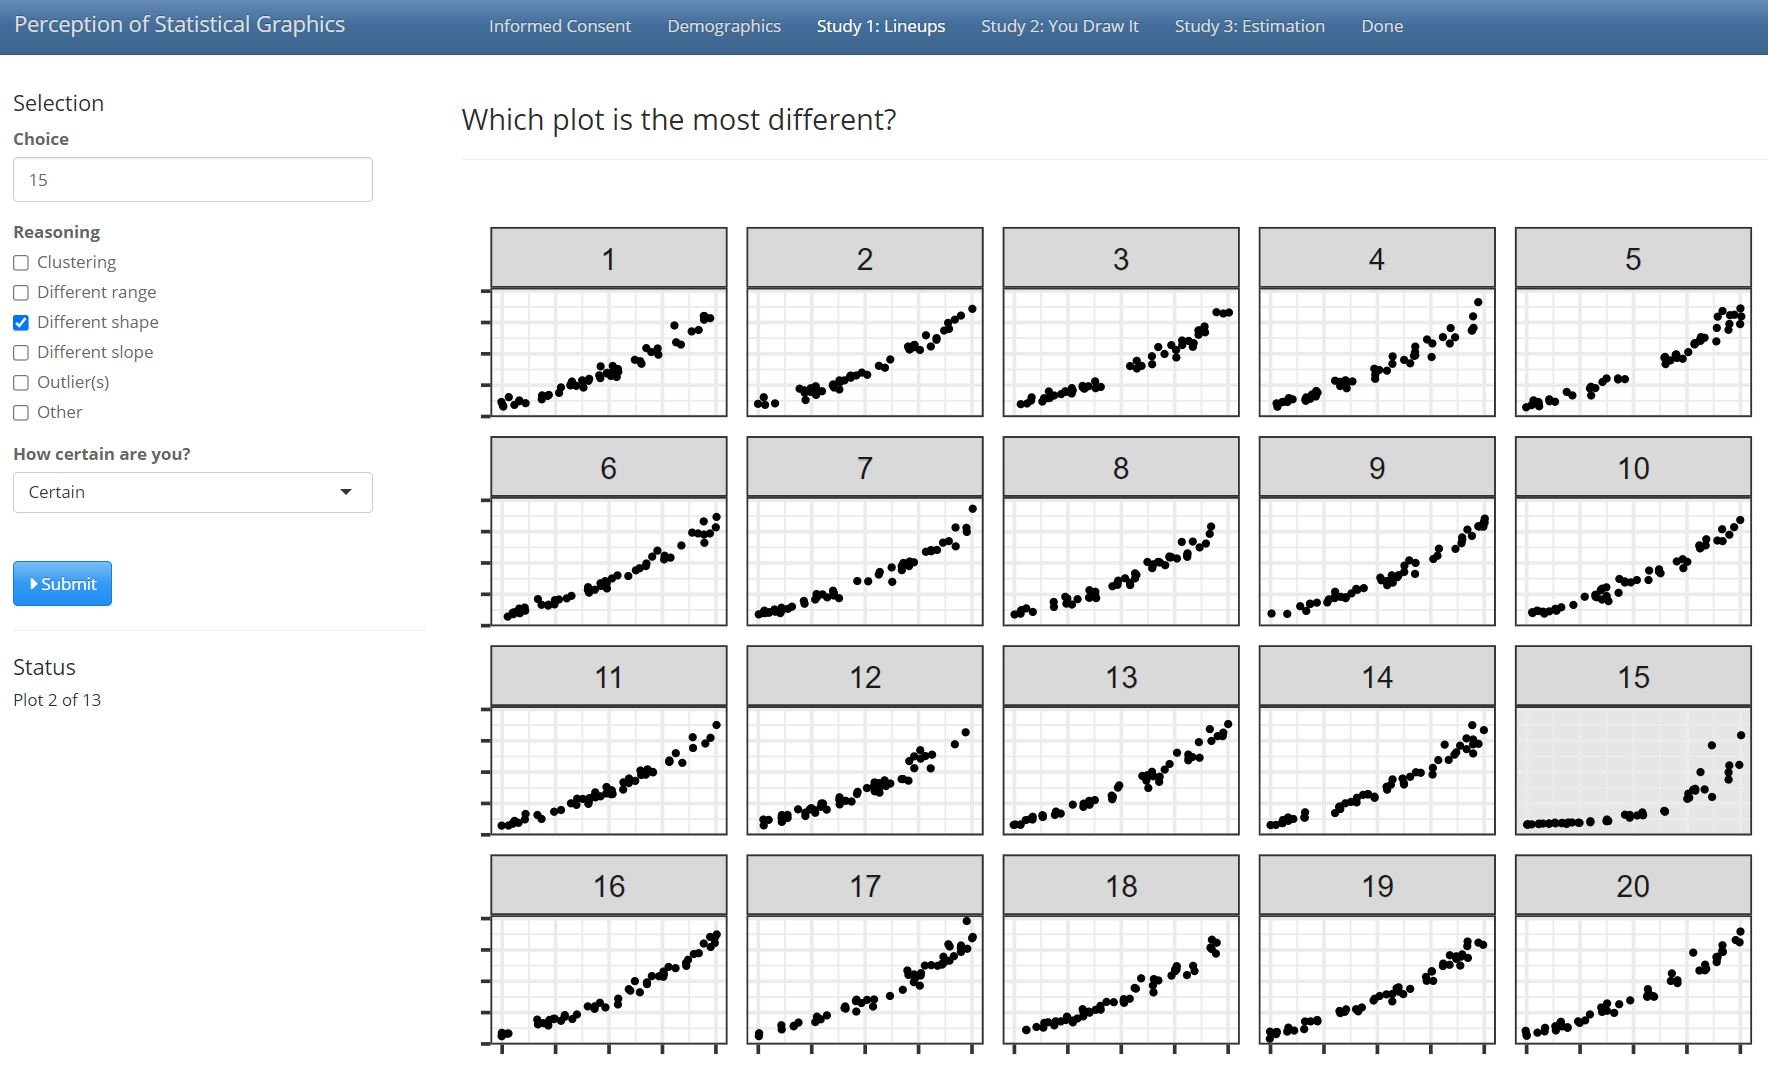
\includegraphics[width=1\linewidth,]{images/lineup-study-example-trial} 

}

\caption{Screenshot of an example trial participants see when completing the lineup study. The applet guided participants through 13 lineup plots and asked them to identify the plot which appeared to be the most different from the others. After participants selected a panel, their choice was highlighted by gray (e.g., Panel 15).}\label{fig:lineup-study-example-trial}
\end{figure}

\subsection{Statistical Analysis}\label{statistical-analysis}

In the first analysis, we aimed to understand our null data generation
process. \citet{vanderplas2021statistical} provides an approach for
calculating the statistical significance of lineups using a Dirichlet
distribution. In particular, we are interested in calculating the
parameter, \(\alpha\), of the Dirichlet distribution that best fits the
``Rorschach'' lineups. An \(\alpha < 0.05\) indicates only one panel in
the lineup was selected more frequently than others, whereas an
\(\alpha > 0.25\) provides support that participant selections are
evenly divided across many interesting panels. We computed the
\(\alpha\) values using the \texttt{estimate\_alpha\_numeric} function
from the vinference R package \citep{Hofmann2020}. This approach allows
us to explore whether any null panels were significantly more unique,
providing insights into the null plot sampling method.

To evaluate participant accuracy of test lineups, each lineup plot
evaluated was assigned a binary value based on the participant response
(correct target plot identification = 1, not correct target plot
identification = 0). We defined \(Y_{ijkl}\) as the event that
participant \(l = 1,...,N_\text{participant}\) correctly identified the
target plot for data set \(k = 1,2\) with curvature combination
\(j = 1,2,3,4,5,6\) plotted on scale \(i = 1,2\). The binary response
was analyzed using a generalized linear mixed model (GLMM) following a
binomial distribution with a logit link function with a row-column
blocking design accounting for the variation due to participant and data
set, respectively, as \begin{equation}
\text{logit }P(Y_{ijkl}) = \eta + \delta_i + \gamma_j + (\delta \gamma)_{ij} + s_l + d_k
\end{equation} \noindent where

\begin{itemize}
\item $\eta$ is the baseline average probability of selecting the target plot
\item $\delta_i$ is the effect of scale $i = 1,2$
\item $\gamma_j$ is the effect of curvature combination $j = 1,2,3,4,5,6$
\item $(\delta\gamma)_{ij}$ is the two-way interaction between the $i^{th}$ scale and $j^{th}$ curvature combination
\item $s_l \sim N(0,\sigma^2_\text{participant})$ is the random effect for participant characteristics
\item $d_k \sim N(0,\sigma^2_{\text{data}})$ is the random effect for data specific characteristics. 
\end{itemize}

\noindent We assumed the random effects for data set and participant are
independent. Target plot identification was analyzed using a GLMM
implemented in \texttt{glmer} from the \texttt{lme4} R (version 4.2.2)
package \citep{lme4}. We used the \texttt{emmeans} R package
\citep{emmeans} to calculate the estimated target detection
probabilities and obtain odds ratio comparisons between the log and
linear scale.

\section{Results}\label{results}

We recruited participants and conducted the study via Prolific, a
crowd-sourcing website, in March 2022. The study included a diverse
group of participants, with an inner-quartile age range between 23 and
31 and a median age of 26 years old. Among the participants, 59\%
self-identified as male, 40\% as female, and 1\% as
variant/nonconforming. Additionally, individuals from more than 21
countries participated in the study and 97\% of the participants
indicated fluency in English. Moreover, 81\% of the participants
reported having completed some undergraduate courses or higher.

\subsection{Rorschach Evaluations}\label{rorschach-evaluations}

\cref{fig:rorschach-lineups} illustrates the selection proportions for
each panel on the ``Rorschach'' lineups corresponding to different
curvature combinations and replicated data sets, when presented on both
log and linear scales. Notably, the panel number is irrelevant, and the
darker shade (bottom) denotes panels chosen more frequently than others.
The plots exhibit relatively even distributions, offering multiple
candidates for the most interesting panel. Additionally, most \(\alpha\)
values are calculated to be above 0.25, indicating participant attention
is divided across multiple interesting panels. It is worth noting that
in the low curvature ``Rorschach'' lineups simulated in data set
replication one, a single panel stands out, with over 50\% of
participants selecting the same null panel on the linear scale and just
under 50\% on the log scale. This particular lineup yields an
\(\alpha = 0.17\) indicating that while the panel selection is not
evenly distributed, there are more than one interesting panel. It is
also worth noting that set two of the low curvature lineup results in a
larger \(\alpha = 0.4.\) High \(\alpha\) values, such as \(\alpha=3.72\)
observed in the low curvature set 2 lineup, reflect a relatively uniform
distribution of participant selections, indicating that multiple panels
attracted similar levels of attention. This suggests the appropriateness
of our null sampling method in producing visually diverse lineups, as
supported by a visual examination of ``Rorschach'' evaluations and the
calculation of \(\alpha\) parameters.

\begin{figure}[tbp]

{\centering 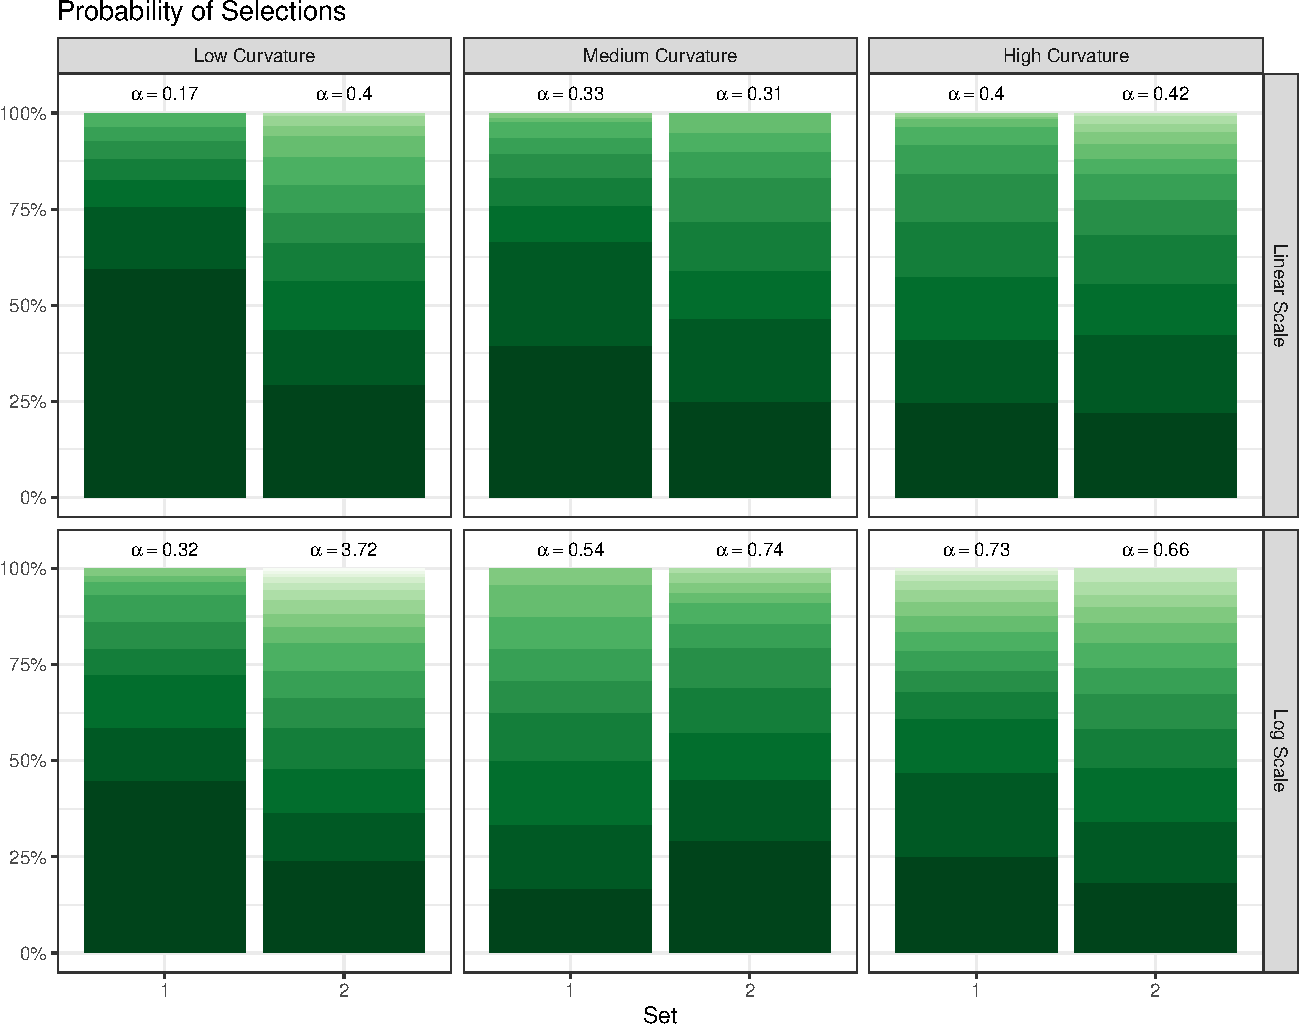
\includegraphics[width=\linewidth,]{logarithmic-lineups-revisions-3_files/figure-latex/rorschach-lineups-1} 

}

\caption{Observed probabilities of panel selections for the 'Rorschach' lineups. The darker shade (bottom) denotes panels chosen more frequently than others. The annotated text provides the calculated $\alpha$ parameter of the Dirichlet distribution that represents individuals' selections for the Rorschach plots.}\label{fig:rorschach-lineups}
\end{figure}

\subsection{Participant Accuracy}\label{participant-accuracy}

During data collection, 325 individuals completed 4,492 individual test
lineup evaluations. We included only participants in the final analysis
who completed the entire study, which included 311 participants and
3,958 lineup evaluations. Due to server capacity, some participants were
required to restart the study, thus resulting in the possibility of more
than twelve lineup evaluations per participant. As a whole, participants
evaluated each uniquely generated lineup plot between 141 and 203 times
(Mean: 164.92, SD: 14.9). Participants correctly identified the target
panel in 47\% of the 1,981 lineup evaluations made on the linear scale
and 65.3\% of the 1,977 lineup evaluations made on the log scale.
\cref{fig:obs-accuracy} shows the observed participant accuracy for each
scale and curvature combination scenario with the dotted line indicating
the average selection percentage for the most picked panel in the
Rorschach lineups for each null curvature model. For example, on
average, we found the medium curvature target model embedded in a
background of low curvature null models have an accuracy rate of 76\% on
the linear scale while the associated top panel selected for low
curvature Rorschach lineups were selected 47.6\% of the time, on
average. We can see from the observed results that participant accuracy
for the linear scale ranged from 3.3\% to 91.6\% while participant
accuracy when identified on the log scale ranges from 46.6\% to 89\%. On
both the log and linear scales, the highest accuracy occurred in lineup
plots where the target model and null model had a considerable
difference in curvature (low curvature target plot embedded in high
curvature null plots; high curvature target plot embedded in low
curvature null plots), and the target plot had more curvature than the
null plots (high curvature target plot embedded in low curvature null
background plots). There was a decrease in accuracy on the linear scale
when comparing a target plot with less curvature to null plots with more
curvature (medium curvature target plot embedded in high curvature null
plots; low curvature target plot embedded in medium curvature null
plots; low curvature target plot embedded in high curvature null plots).
Additionally, accuracy increased when data was displayed on the log
scale compared to the linear scale in all curvature scenarios with an
exception of a medium target curve embedded in low null curves. The
dotted lines in \cref{fig:obs-accuracy} indicate that the average
selection percentage for the top panels in the Rorschach lineups range
from 22.8\% to 47.6\%. Given all panels in the Rorschach lineups were
generated under the same model, this random selection highlights the
variability in null plots due to random data generation. When pairing
the accuracy with the selection percentage for the top picked panel from
the Rorschach lineups, we can see that accuracy is higher than the
randomly selected top Rorschach panel when presented on the log scale
for all curvature combinations. However, when comparing accuracy to the
top picked panel from the Rorschach lineups on the linear scale,
accuracy of selections for low target panels when embedded in medium
curvature background null panels and medium target panels embedded in
high curvature background null panels is no better than the selection
percentage for the top Rorschach panels associated with the null models;
in these two cases, the variability in the null plots overpowers the
actual trend differences. In other words, the linear scale appears to
amplify the differences that are spurious due to random noise, such as
outliers, in addition to amplifying the data trend. In contrast, the log
scale minimizes the spurious differences due to random noise in favor of
the differences due to trends in the data. As we replicated each
curvature combination and Rorschach lineups with two sets in order to
understand the variability, we can (minimally) examine both due to the
data mean and variability in plot selections due to the data generation
process. The appendix includes the number of selections for lineup plots
from the study where the variability dominates the curvature trends
found in the data.

In addition to participant accuracy, we conducted a linear mixed model
on participant confidence (5 - Very Certain to 1 - Very Uncertain). We
found that, on average, individuals who were correct are 0.556 (se
0.039) Likert scale points more confident than individuals who were
incorrect in their plot choice across all conditions (F = 214.57; df =
1, 3709; p \textless{} 0.0001). Similarly, on average, lineups evaluated
on the log scale indicated participants were only 0.075 (se 0.0366)
Likert scale points more confident than lineups evaluated on the linear
scale (F = 3.70; df = 1, 3709; p = 0.054). We discuss further details
regarding selection reasoning and confidence level in the appendix.

\begin{figure}[tbp]

{\centering 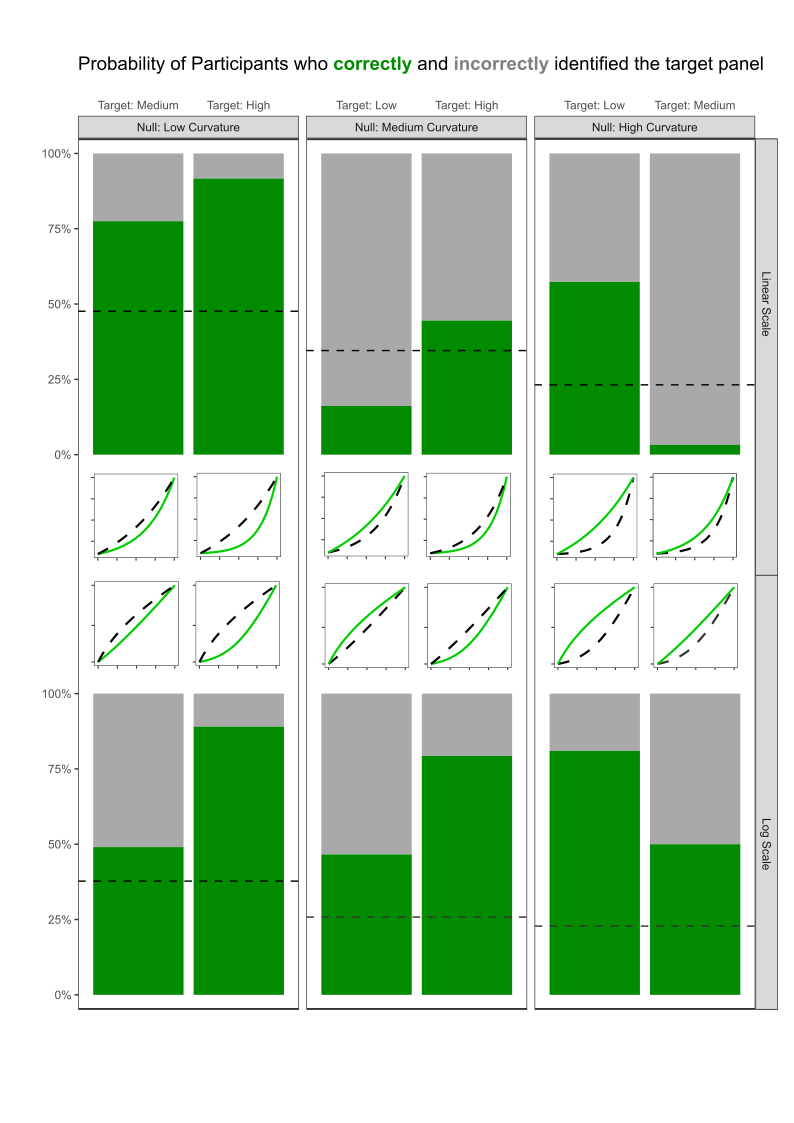
\includegraphics[width=\linewidth,]{images/observed-probabilities} 

}

\caption{The observed accuracy for identifying the target panel for each curvature combination scenario with the accuracy for the linear scale shown on the top and the accuracy for the log scale shown on the bottom. The thumbnail figures below each plot display the curvature combination as shown in \cref{fig:curvature-combination-example} on both scales. The most selected rorschach panel percentage averaged for each null background curavature and scale is shown by the dotted line.}\label{fig:obs-accuracy}
\end{figure}

The results from the GLMM on participant accuracy indicated a strong
interaction between the curvature combination and scale
(\(\chi^2_5 = 294.443\); \(\text{p} <0.0001\)), and the estimated
variance due to participant and data set were
\(\hat\sigma^2_{\text{participant}} = 1.19\) (s.e. = 1.09) and
\(\hat\sigma^2_{\text{data}} = 0.433\) (s.e. = 0.66), respectively.
Therefore, we concluded that there was low variability in the accuracy
of target panel detection between participants and across replications
of uniquely simulated data sets. To determine the effect of scale, we
compared the estimated accuracy between the log and linear scale within
each curvature combination due to the interaction as determined by the
GLMM.

\cref{fig:odds-ratio-plot} displays the estimated (log) odds ratio of
successfully identifying the target panel on the log scale compared to
the linear scale. The thumbnail figures to the right of the plot
illustrate the curvature combination on the linear (left thumbnail) and
log base ten (right thumbnail) scales associated with the \(y\)-axis
label. The choice of scale had no impact if the curvature differences
were substantial and the target plot had more curvature than the null
plots (high curvature target plot embedded in low curvature null plots).
However, presenting data on the log scale makes us more sensitive to
slight changes in curvature (low or high curvature target plot embedded
in medium curvature null plots; medium curvature target plot embedded in
high curvature null plots) and apparent differences in curvature when
the target plot had less curvature than the null plots (low curvature
target plot embedded in high curvature null plots). An exception
occurred when identifying a plot with curvature embedded in null plots
close to a linear trend (medium curvature target panel embedded in low
curvature null panels). The results indicate that participants were more
accurate at detecting the target panel on the linear scale than on the
log scale. When examining this curvature combination, the same
perceptual effect occurred as we previously saw, but in a different
context of scales. On the linear scale, participants were perceptually
identifying a convexly curved trend from close to a linear trend,
whereas after the logarithmic transformation, participants were
perceptually identifying a trend close to linear from a concavely curved
trend (\cref{fig:curvature-combination-example}).

\begin{figure}[tbp]

{\centering 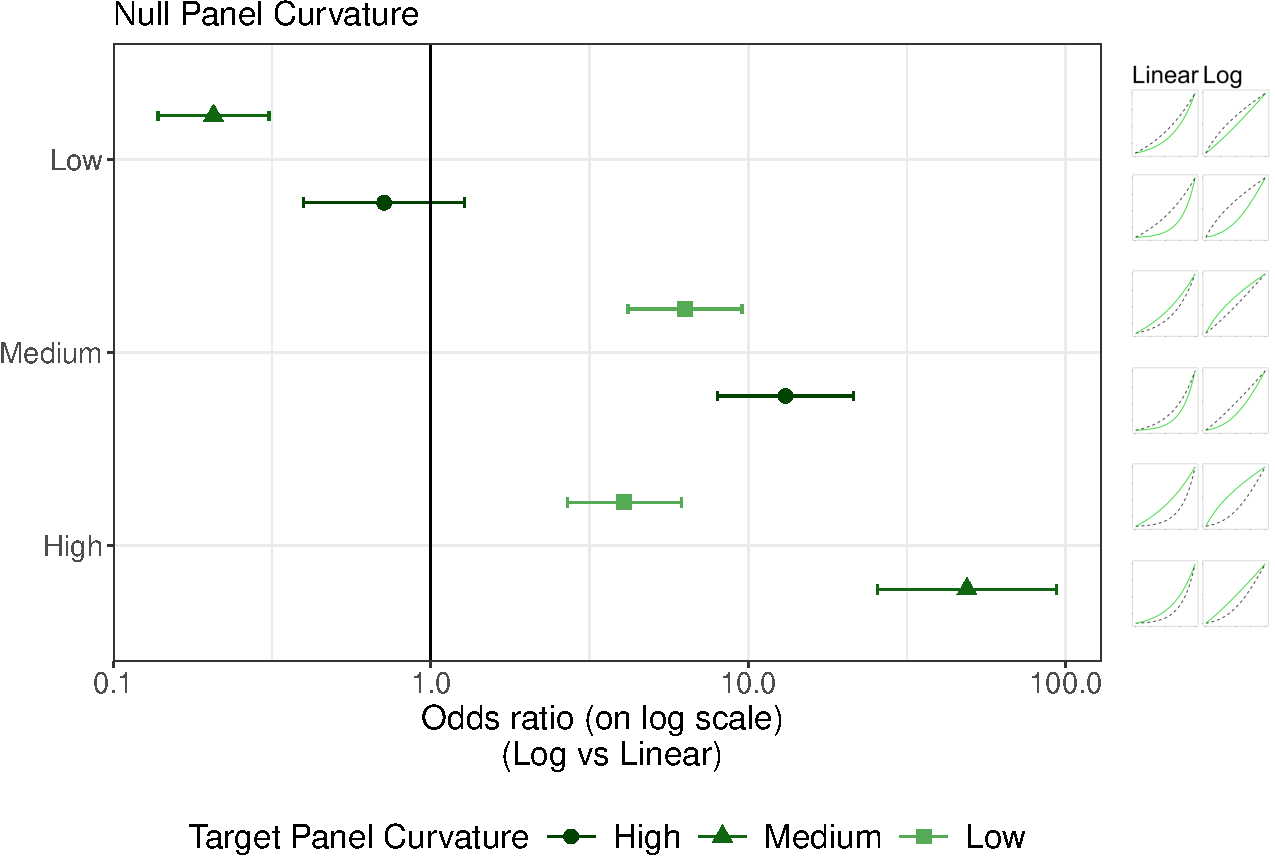
\includegraphics[width=\linewidth,]{logarithmic-lineups-revisions-3_files/figure-latex/odds-ratio-plot-1} 

}

\caption{Estimated (log) odds ratio of successfully identifying the target panel on the log scale compared to the linear scale. The y-axis indicates the model parameters used to simulate the null plots with the target plot model parameter selection designated by shape and shade. The thumbnail figures on the right display the curvature combination as shown in \cref{fig:curvature-combination-example} on both scales (linear - left, log - right).}\label{fig:odds-ratio-plot}
\end{figure}

\section{Discussion and Conclusion}\label{discussion-conclusion}

This work aims to provide foundational research to support the
principles that guide design decisions in scientific visualizations. In
this study, we explored the perceptual sensitivities of detecting
differences between curvature levels as altered by the choice of scale.

The results indicated that when there was a considerable difference in
curvature between the target plot and null plots and the target plot had
more curvature than the null plots, the choice of scale had no impact,
and participants accurately differentiated between the two curves on
both the linear and log scale. However, due to the altered appearance of
the data, displaying exponentially increasing data on a log scale
improved the accuracy of differentiating between models with slight
curvature differences or apparent curvature differences when the target
plot had less curvature than the null plots. An exception occurred when
identifying a plot with curvature embedded in surrounding plots
perceived close to a linear trend. The thumbnail figures in
\cref{fig:obs-accuracy} visually demonstrate the opposing perceptual
behaviors of the curves for a medium target curve embedded in low null
curves displayed on the two different scales. This result supports the
findings by \citet{best_perception_2007}, who found that the accuracy of
identifying the correct curve type was higher when presented with
nonlinear trends, indicating that it is hard to say something is linear
(i.e., something has less curvature), but easy to say that it is not
linear; our results concur with this observation. Therefore, in the
context of this study, it is easy to identify a curve in a group of
lines but harder to identify a line in a group of curves.

Using visual inference to identify these guidelines suggests that it is
important to consider the appearance of curves as altered by the choice
of scale when identifying differences between data. In the specific case
of this study and selected data simulation equations, we found a slight
advantage of using the log transformation when curvature differences
were small due to the way the log scale changed the appearance of the
curves. This aligns with findings by \citet{dresp20152d}, who
demonstrated that the human visual system has an in-built sensitivity to
local curve geometry, indicating that the visual perception of curvature
can be significantly influenced by geometric transformations such as log
scaling. The most frequent panel selection percentage from the Rorschach
lineups indicates the linear scale highlights random variability in
favor of the curvature trend while the log scale suppresses the spurious
differences in favor of the actual trend differences in data.

It is worth noting that our study focused specifically on data simulated
with a two-parameter exponential function with a shift and such
conclusions may not be broadly applicable to other functions or
different parameterizations of exponential data resulting in curvature.
This scenario, while fairly specific, lays the perceptual groundwork for
more investigation into the use of log scales with exponential data. Now
that we know how curvature can be distinguished, it's easier to conduct
follow up studies that cover more scenarios and use different graphical
testing methods.

We conducted this study as the first in a series of three graphical
tests to understand the perceptual and cognitive implications of using
log scales to display exponentially increasing data. Previous research
by \citet{ciccione2022analyzing} found that individuals often
underestimate exponential growth when presented values numerically and
graphically, highlighting the need for better understanding and
presentation of such data. In our next two papers in this series, we
will investigate whether using log scales presents cognitive
disadvantages, such as making it harder to utilize graphical
information. \citet{lammers2020correcting} showed that correcting
exponential growth bias could significantly increase support for social
distancing, suggesting that improving the accuracy of visual
representations of exponential growth can have substantial real-world
impacts.

These studies serve as an example of multi-modal graphical testing,
examining different levels of engagement and interaction with graphics
in order to produce nuanced, specific guidelines for graphical design.
By testing graphics in situations similar to how they are used in
practice, we can gain additional insight into graphical perception and
improve visual communication of scientific results.

\section*{Supplementary Material}\label{supplementary-material}
\addcontentsline{toc}{section}{Supplementary Material}

\begin{itemize}
\tightlist
\item
  \textbf{Participant Data:} De-identified participant data collected in
  the study and used for analyses (lineup-model-data.csv).
\item
  \textbf{Data Analysis Code:} The code used to replicate the analysis
  in this paper (lineups-analysis.qmd).
\item
  \textbf{Study Applet Code:} The code used to create the study applet
  via RShiny can be found on GitHub at
  \url{https://github.com/earobinson95/perception-of-statistical-graphics-log}
\item
  \textbf{README:} File containing detailed descriptions of the
  supplementary material. (README.html).
\end{itemize}

\newpage

\renewcommand{\thesection}{A}
\setcounter{figure}{0}    
\renewcommand\thefigure{\thesection\arabic{figure}}  
\setcounter{equation}{0}    
\renewcommand\theequation{\thesection\arabic{equation}}

\section{Exponential growth rates and
curvature}\label{exponential-growth-rates-and-curvature}

Let us consider a simple equation, distinct from the one employed to
simulate data in our study. This equation can be used to simulate data
which grows exponentially in \(x\), with optional error term
\(\epsilon\):
\begin{align}y &= \exp\{\beta_1 x + \epsilon\}\quad \text{where}\quad \epsilon \sim N(0, \sigma).\label{eq:simpleexp}\end{align}

\begin{figure}[hb]

{\centering 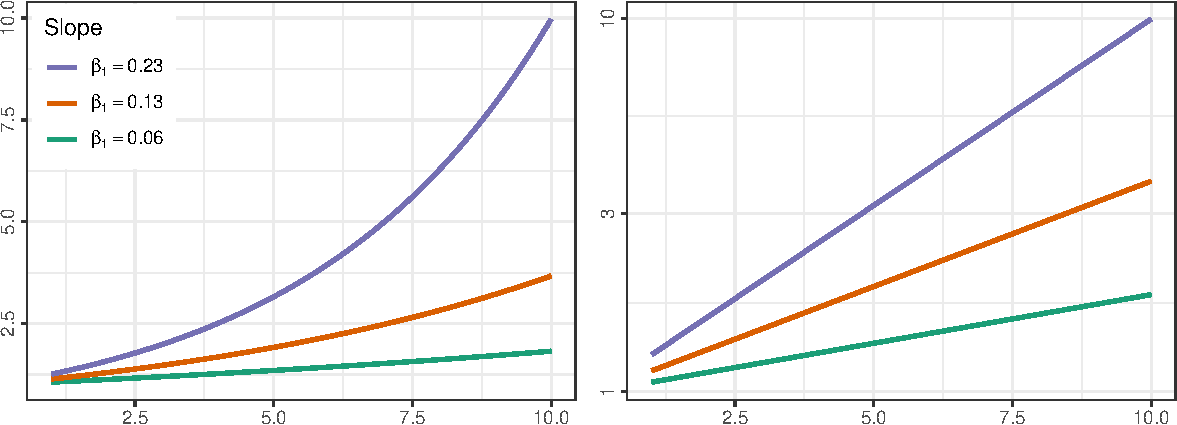
\includegraphics[width=\linewidth,]{appendix-3_files/figure-latex/simple-exponential-1} 

}

\caption{Linear and log scale simple exponential equations as specified in \cref{eq:simpleexp}, with error term excluded. The y-axis endpoints are a primary visual signal when differentiating between the lines in both plots.}\label{fig:simple-exponential}
\end{figure}

It is important in lineup studies to control for extraneous visual
signals, and when other visual signals creep in, results of the study
can be difficult to interpret \citep{vanderplas_clusters_2017}.

In this particular case, the extraneous visual signals are the endpoints
of the lines (the endpoint at \(x=10\) on a linear scale, and both
endpoints on the log scale), as shown in \cref{fig:simple-exponential}.
Preattentive features guide attention
\citep{wolfeWhatPreattentiveFeature2019}; one of the first things we do
when scanning a graph is to notice the extent of the data within the
axes. We must control the endpoints to ensure that participants are
using active attention to assess the lineup and draw conclusions, so
that the whole visual signal is processed as part of the lineup
evaluation; if participants are making decisions off of the endpoints,
then we cannot interpret the results to say that they are assessing the
rate of exponential growth rather than the end result.

There are several different options for controlling the visual signal in
a lineup:

\begin{enumerate}
\def\labelenumi{\arabic{enumi}.}
\setcounter{enumi}{-1}
\tightlist
\item
  Do nothing and set each subplot's limits to the overall maximum
  limits.
\item
  allow each subplot to have different axis limits
\item
  truncate the displayed range of each subplot to the minimum range
  generated in the lineup
\item
  add extra parameters to the exponential equation to adjust the range
  of the data so that it fits within a pre-specified domain, as in
  \cref{alg:lineup-exponential-data-simulation-algorithm}.
\end{enumerate}

\begin{figure}[tbp]

{\centering 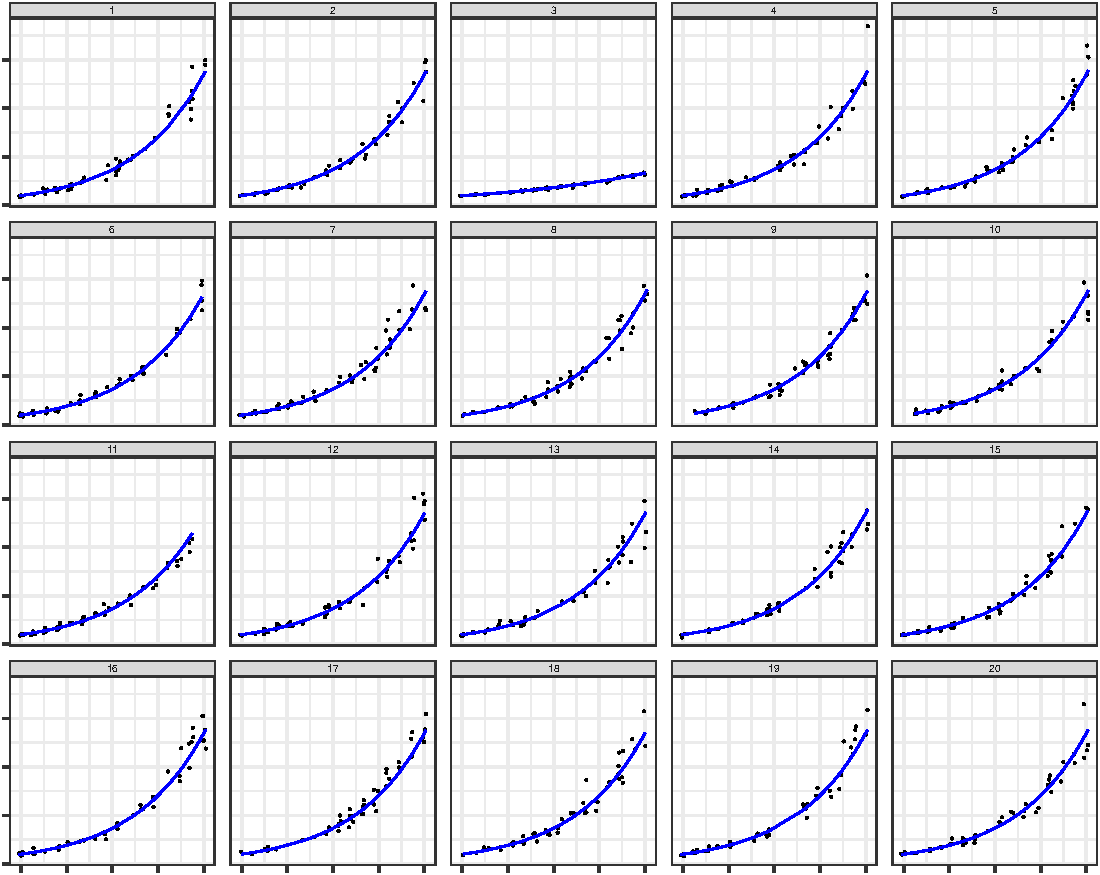
\includegraphics[width=.6\linewidth,]{appendix-3_files/figure-latex/lineup-fixed-scales-1} 

}

\caption{When axis limits are fixed to the most expansive extent in the generated data, the primary signal becomes the extent of the domain which has data, rather than the growth rate itself.}\label{fig:lineup-fixed-scales}
\end{figure}

Typically, lineups do not show axis labels or scaling, because the goal
is to assess the signal from the data without additional context. In
addition, the traditional 20-panel lineup would be quite visually
confusing in this circumstance:

\begin{figure}[tbp]

{\centering \subfloat[Lineup\label{fig:lineup-free-scales-1}]{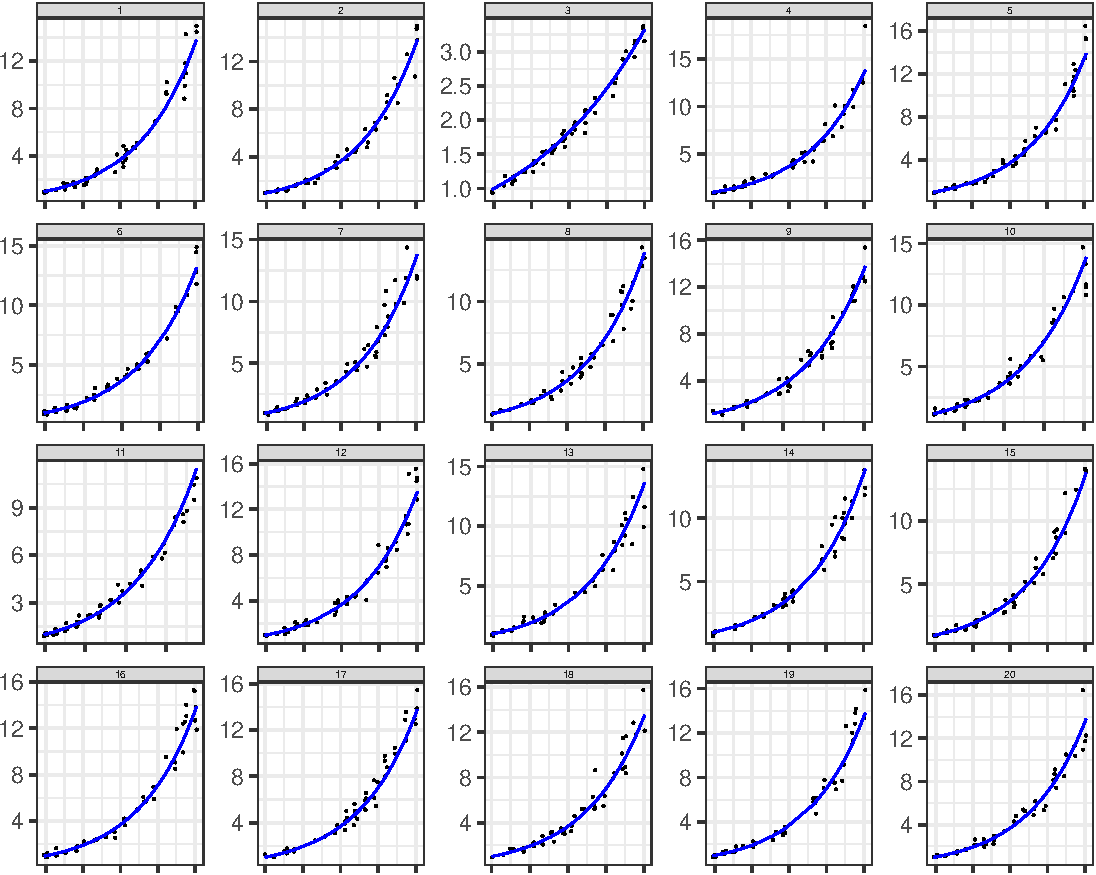
\includegraphics[width=.6\linewidth,]{appendix-3_files/figure-latex/lineup-free-scales-1} }\subfloat[Overlay of null and signal panels.\label{fig:lineup-free-scales-2}]{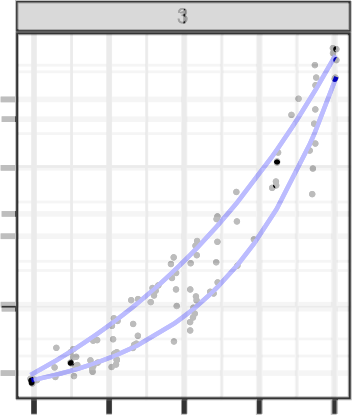
\includegraphics[width=.2\linewidth,]{images/curvature-overlay-free-scales} }

}

\caption{When y-axis limits vary by panel, the y-axis labels are the primary visual signal; the secondary signal (when the panels are overlaid) is the curvature of the line.}\label{fig:lineup-free-scales}
\end{figure}

\cref{fig:lineup-free-scales} demonstrates that when we ignore the
y-axis labels and overlay the signal panel with one of the null panels,
the remaining difference is the curvature of the line. If we want to
keep the standard convention of not including y-axis labels in lineups
for simplicity and to reduce plot clutter, this alternative signal seems
promising (and as we will show, is approximately equivalent to option
3).

Let us next consider option 2: Crop each panel to the minimum limits of
all generated data. The result is shown in
\cref{fig:lineup-truncate-scales}. This operation shifts which axis
becomes the visually important factor, but doesn't change the problem:
previously the issue was the y-axis extent, now it is the x-axis extent.
Both of these parameters are implicitly affected by how we generate
exponential data. In order to truly assess whether people can
discriminate between comparable exponential growth rates graphically, it
is more useful to approach the problem from a curvature perspective
rather than to artificially limit the data shown.

This issue is a fundamental problem when testing graphics: the test must
meet the ``goldilocks'' standard - not too hard, not too easy, but just
right. Both option 0 and option 2 fail this standard.

\begin{figure}[tbp]

{\centering 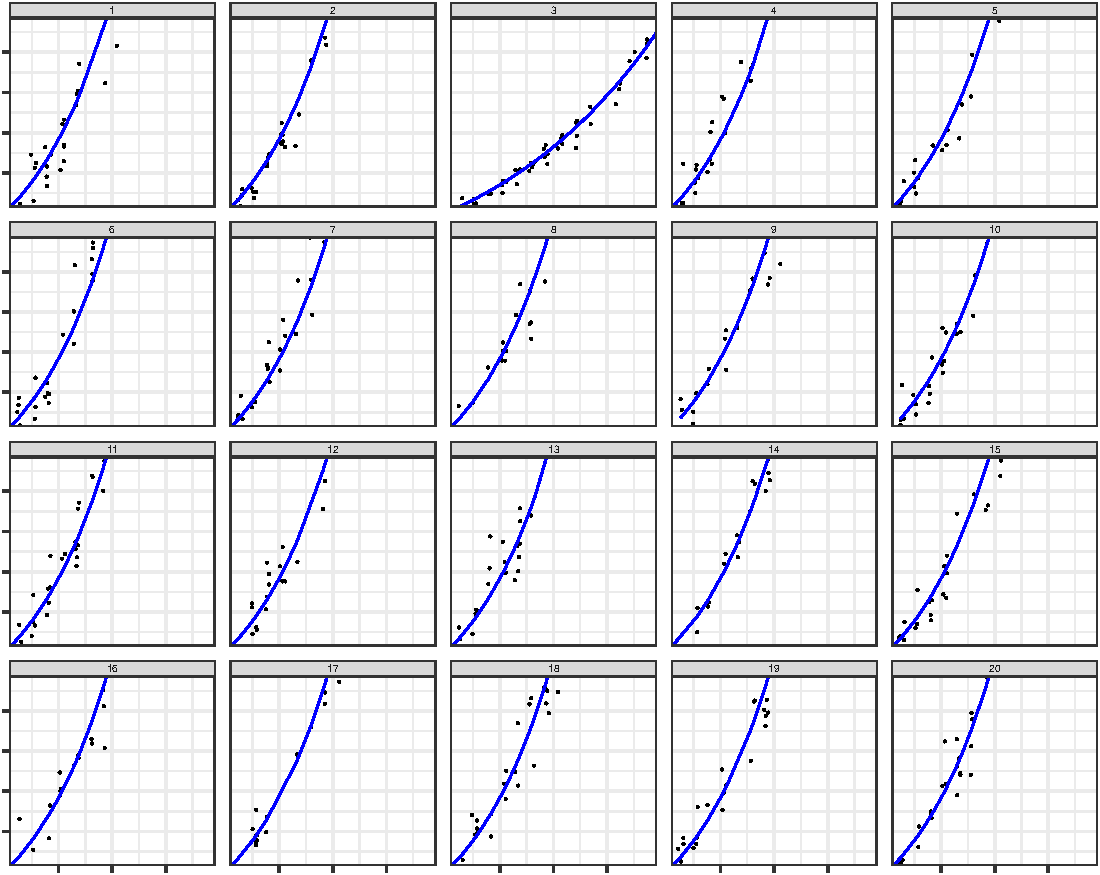
\includegraphics[width=.6\linewidth,]{appendix-3_files/figure-latex/lineup-truncate-scales-1} 

}

\caption{When axis limits are fixed to the most restrictive in all generated data, the primary signal becomes the extent of the x axis which is covered with data, rather than the growth rate itself.}\label{fig:lineup-truncate-scales}
\end{figure}

Visually, both the \(x\) and \(y\) axes matter equally, even if it might
on paper make sense to truncate \(x\) in order to control the \(y\) axis
range.

An additional benefit of controlling endpoints is that it also provides
some realism: our goal was to assess the ability to examine exponential
growth \textbf{rates}, motivated by the COVID-19 pandemic. As each
geographic reporting region started with different numbers of cases and
had different control policies, the \(\alpha\) and \(\theta\) parameters
are reasonable to represent some of these differences while still
examining the underlying exponential behavior.

To control these endpoints on both scales then we have to move to an
exponential model that is a bit more complicated:
\begin{align}y = \alpha \cdot \exp\left\{\beta_1 x + \epsilon\right\} + \theta\quad \text{where}\quad \epsilon \sim N(0, \sigma).\label{eq:complexexp}\end{align}

\(\alpha\) and \(\theta\) were used to make endpoints consistent among
the growth rates. As a result, the lineups examine the degree of
inflection of the trend rather than the explicit exponential growth
rate. An explanation for how the ultimate values for \(\alpha\) and
\(\theta\) were determined is provided in
\cref{alg:lineup-exponential-data-simulation-algorithm}.
\cref{fig:lineup-scale-data} uses the parameters in
\cref{tab:parameter-data} and the data generating method described in
\cref{alg:lineup-exponential-data-simulation-algorithm}. The result is a
series of panels which have obvious variation due to the points (a
desirable feature) but where the underlying relationship shown in blue
has consistent endpoints. As a result, the question becomes whether
participants can identify that plot 3 has a different growth rate (as
measured by the curvature of the line).

\begin{figure}[tbp]

{\centering 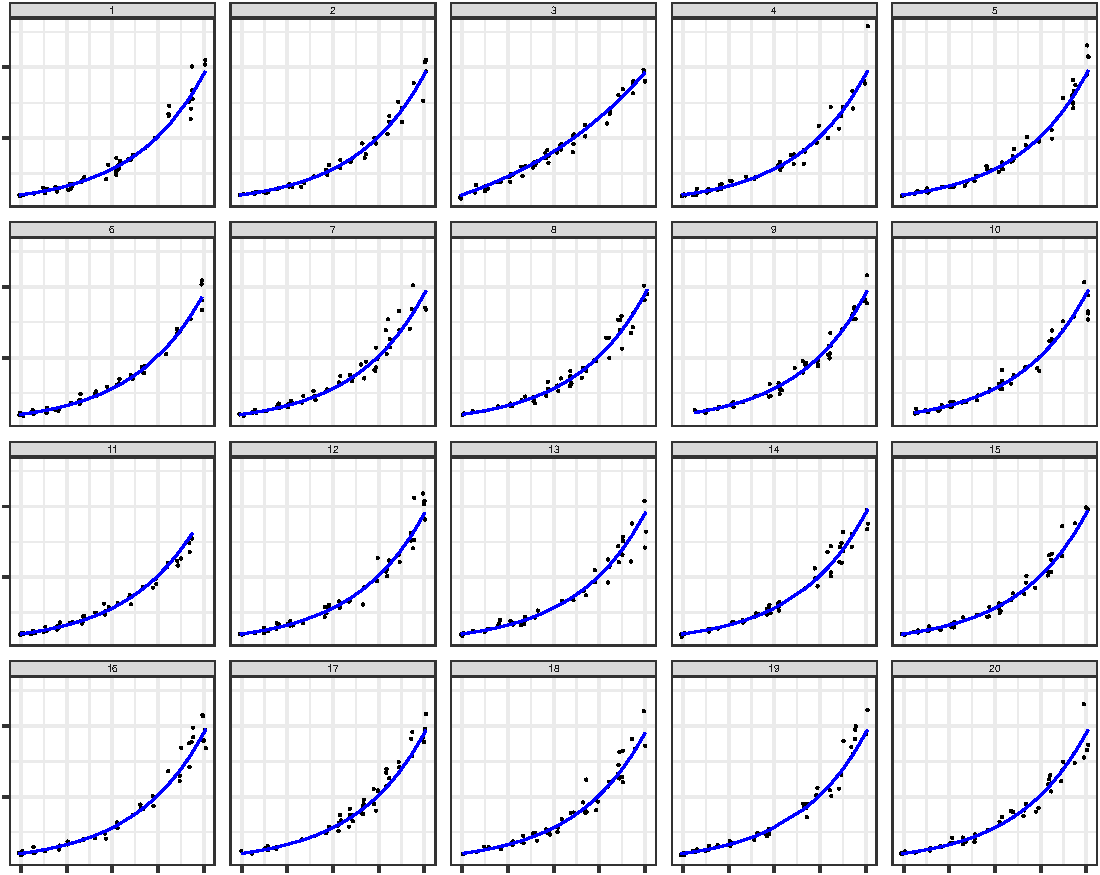
\includegraphics[width=.6\linewidth,]{appendix-3_files/figure-latex/lineup-scale-data-1} 

}

\caption{When the data are scaled such that endpoints are similar across all conditions, the primary feature becomes the curvature of the line, while individual plots show random variation due to the scatter around the line.}\label{fig:lineup-scale-data}
\end{figure}

\renewcommand{\thesection}{B}

\section{Participant confidence and
accuracy}\label{participant-confidence-and-accuracy}

In addition to investigating how scale and curvature rate influence
participant accuracy, we asked participants to indicate their level of
confidence on a five-point Likert scale by answering, ``How certain are
you?'' \cref{fig:conf-mosaic} shows the observed confidence rating
proportions for correct and incorrect identifications across the
different scale and curvature combination scenarios. We conducted a
linear mixed model using the lmer function from the lme4 \citep{lme4} R
package in order to determine how participant confidence (5 - Very
Certain to 1 - Very Uncertain) varied across conditions. We included
curvature combination, scale, accuracy (correct or incorrect), and all
two- and three-way interactions along with a random participant effect.
While there are limitations to assuming normality of Likert scale data,
we evaluated model fit by observing residuals and comparing the results
to non-parametric and multinomial methods. Due to the interpretability
of the linear mixed model, we proceed to present the findings from this
analysis. Overall, on average, individuals who were correct are 0.556
(se 0.039) Likert scale points more confident than individuals who were
incorrect in their plot choice across all conditions (F = 214.57; df =
1, 3709; p \textless{} 0.0001). We did not find convincing evidence of a
discernable difference in confidence levels between scales (F = 3.70; df
= 1, 3709; p = 0.054). Overall, on average, lineups evaluated on the log
scale indicated participants were 0.075 (se 0.0366) Likert scale points
more confident than lineups evaluated on the linear scale.

\begin{figure}[H]

{\centering 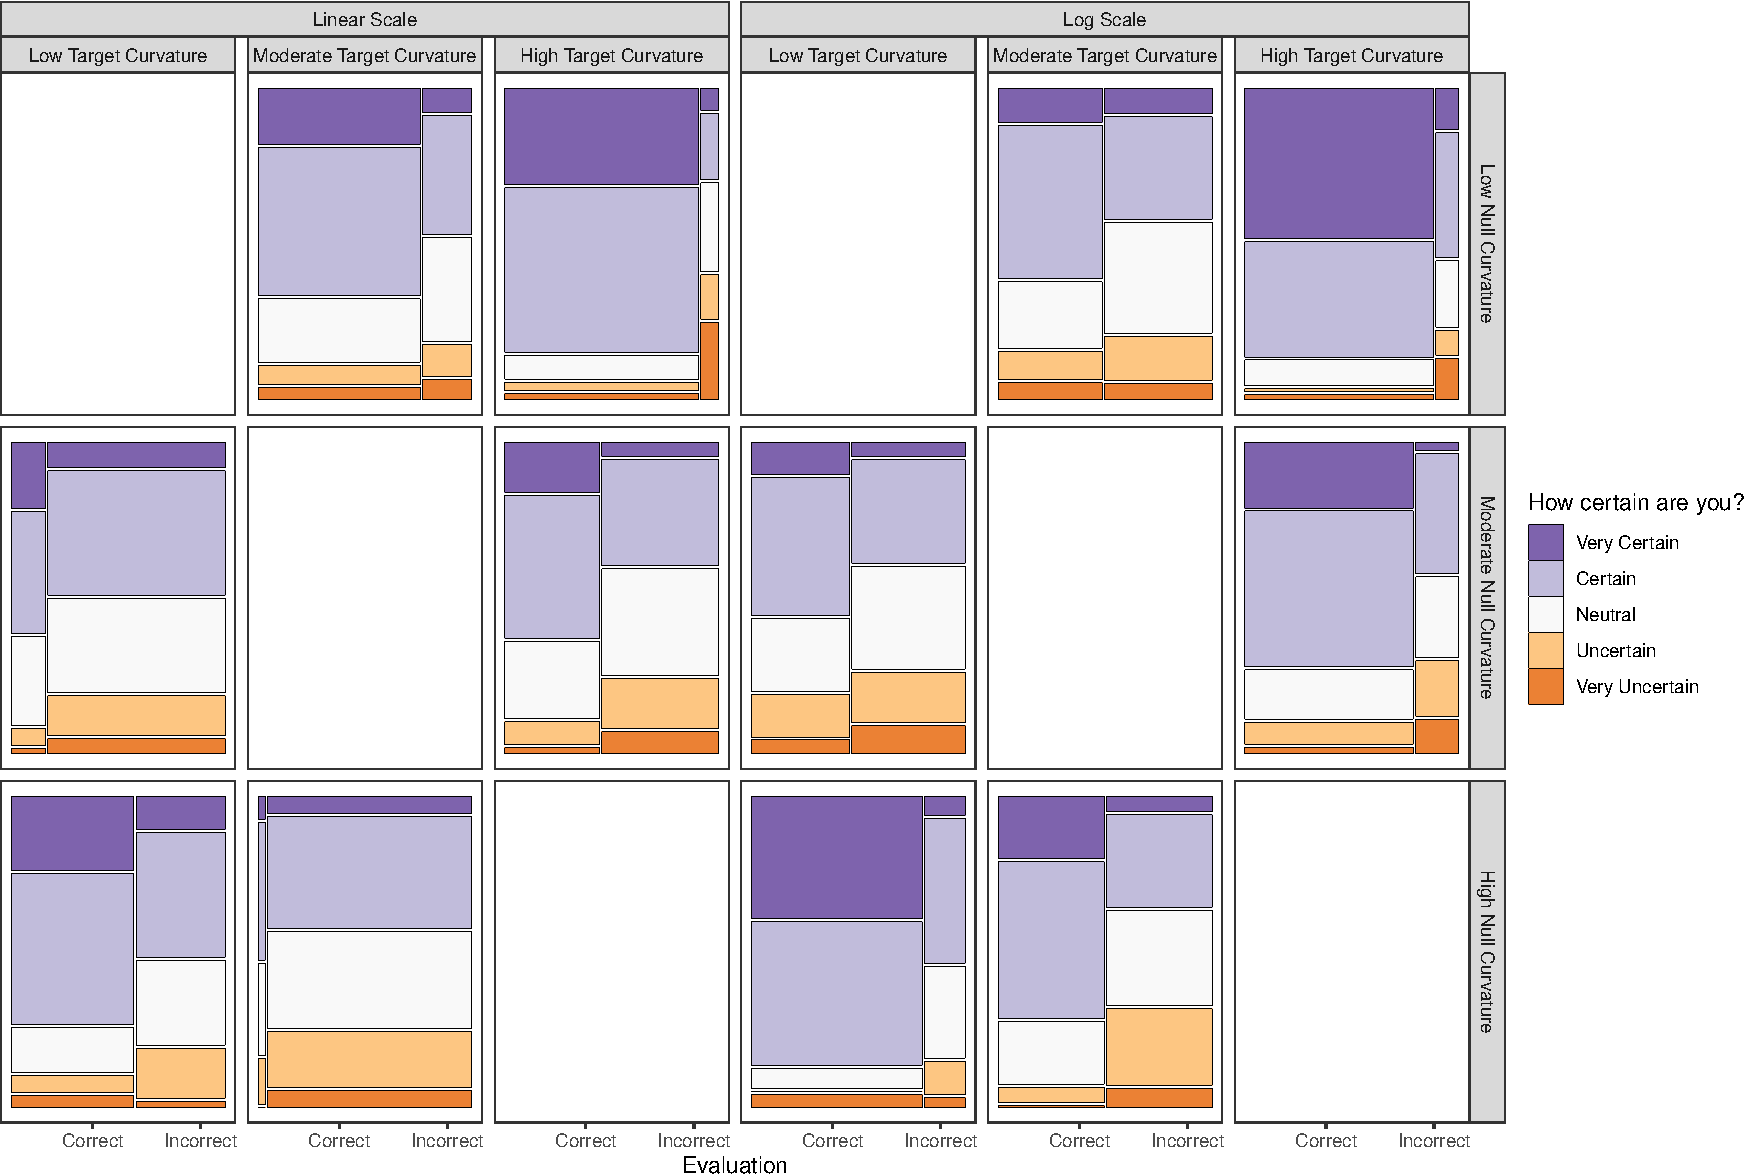
\includegraphics[width=\linewidth,]{appendix-3_files/figure-latex/conf-mosaic-1} 

}

\caption{Observed proportion of evaluations for each confidence rating (five-point Likert scale) by accuracy. The width of the bars indicates the number of evaluations for correct and incorrect identifications within each curvature combination.}\label{fig:conf-mosaic}
\end{figure}

\renewcommand{\thesection}{C}

\section{Participant selections of lineup
panels}\label{participant-selections-of-lineup-panels}

We simulated a total of 18 data sets (twelve test data sets and six
Rorschach data sets) and plotted on both the linear scale and the log
scale (36 lineup plots). Each parameter combination was generated in
sets of two in order to account for variability in simulating data with
random errors. The following plots display each of the lineups created
for the study for the associated null background curvature model with
the number of evaluation panel selection counts overlaid (circle = null
panels; rectangle = target panel). In particular, set 2 for a high
curvature target panel embedded in medium curvature background null
panels highlights the outliers in the target plot (panel 14) on the
linear scale while the log scale for the same data set suppresses the
visual display of the outliers. By inspecting the lineups alongside the
number of evaluations per panel, we can further understand whether
participant's made their selection based on spurious differences due to
random noise or the curvature trend of the data.

\subsection{Low Curvature Null
Background}\label{low-curvature-null-background}

\begin{center}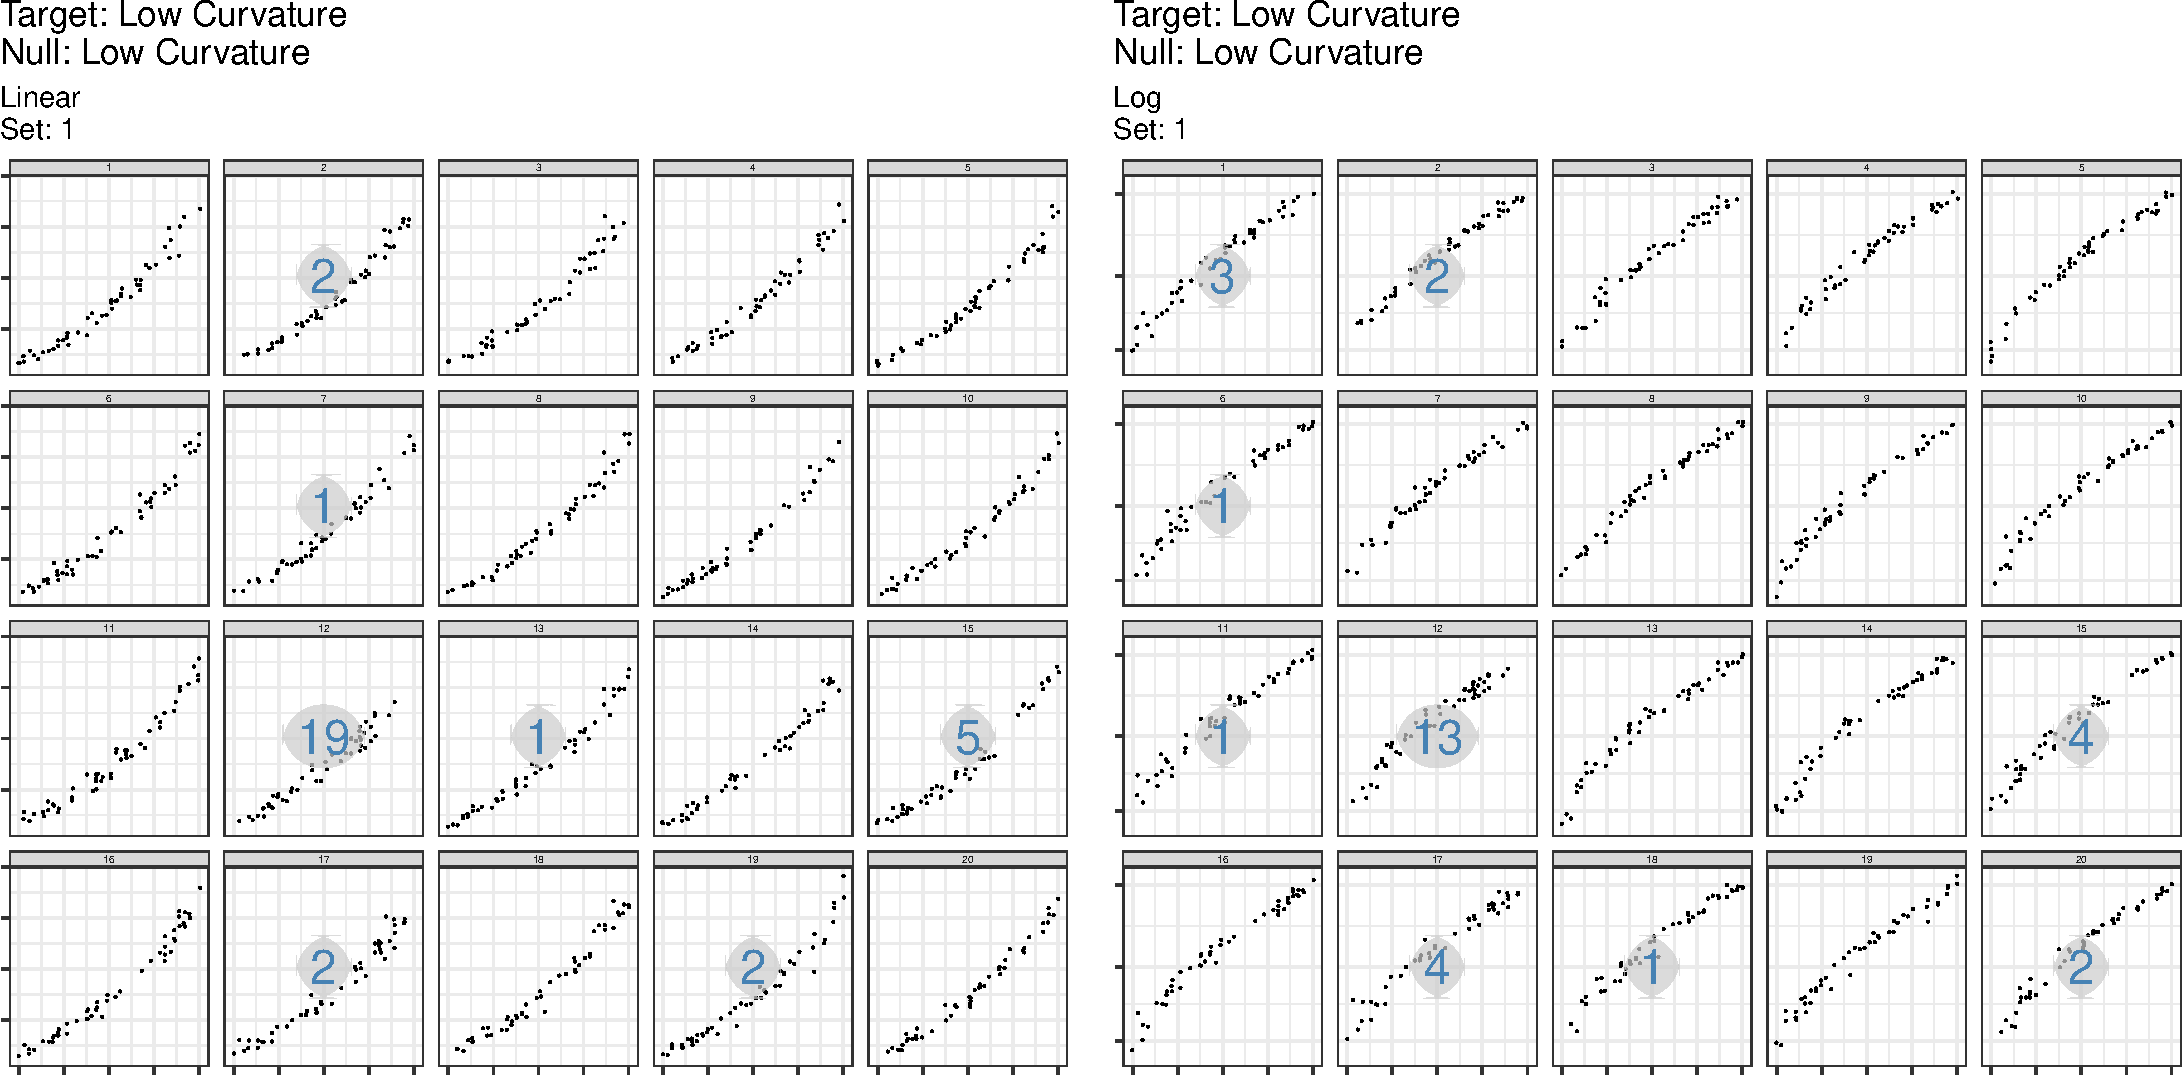
\includegraphics[width=\linewidth,]{appendix-3_files/figure-latex/unnamed-chunk-4-1} \end{center}

\begin{center}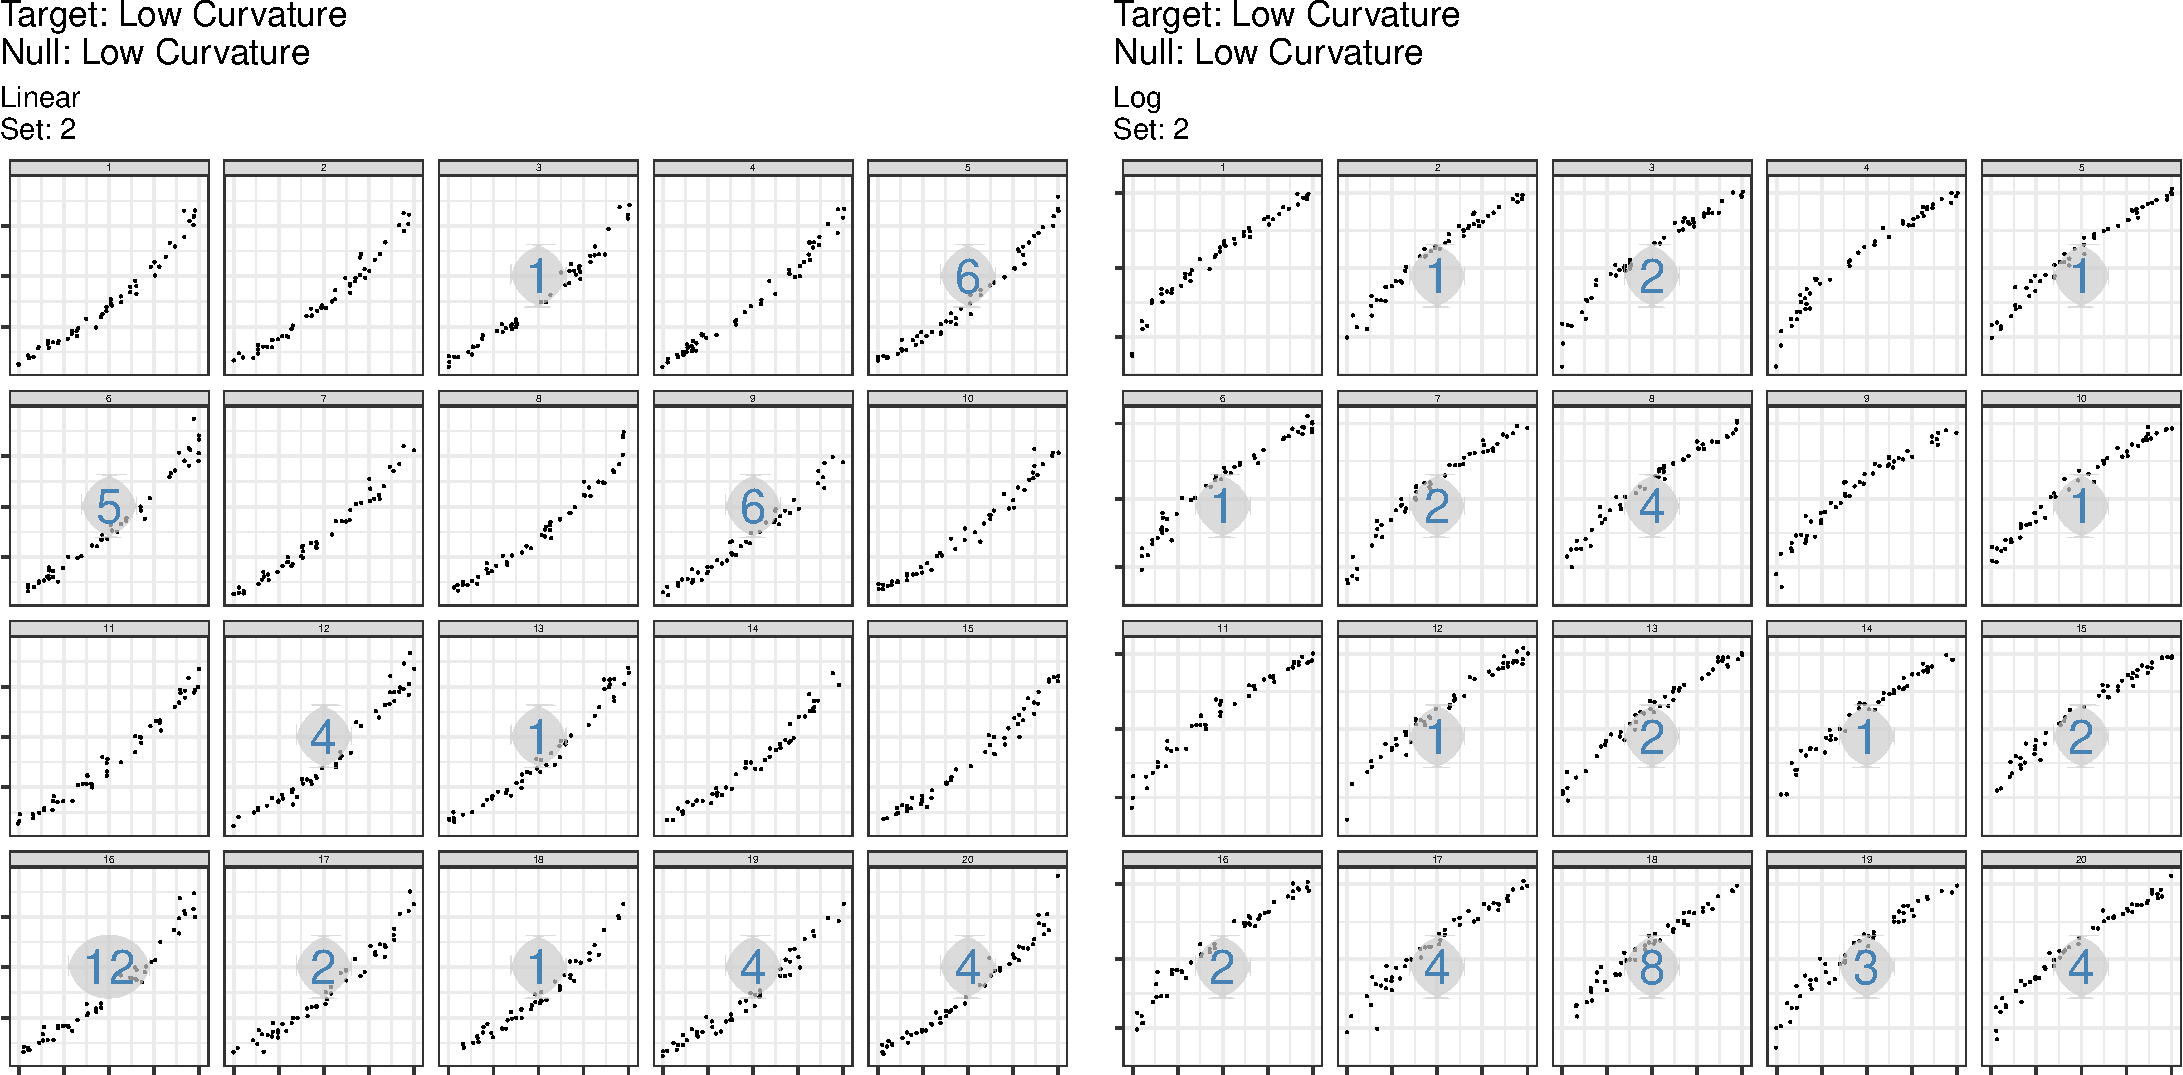
\includegraphics[width=\linewidth,]{appendix-3_files/figure-latex/unnamed-chunk-4-2} \end{center}

\begin{center}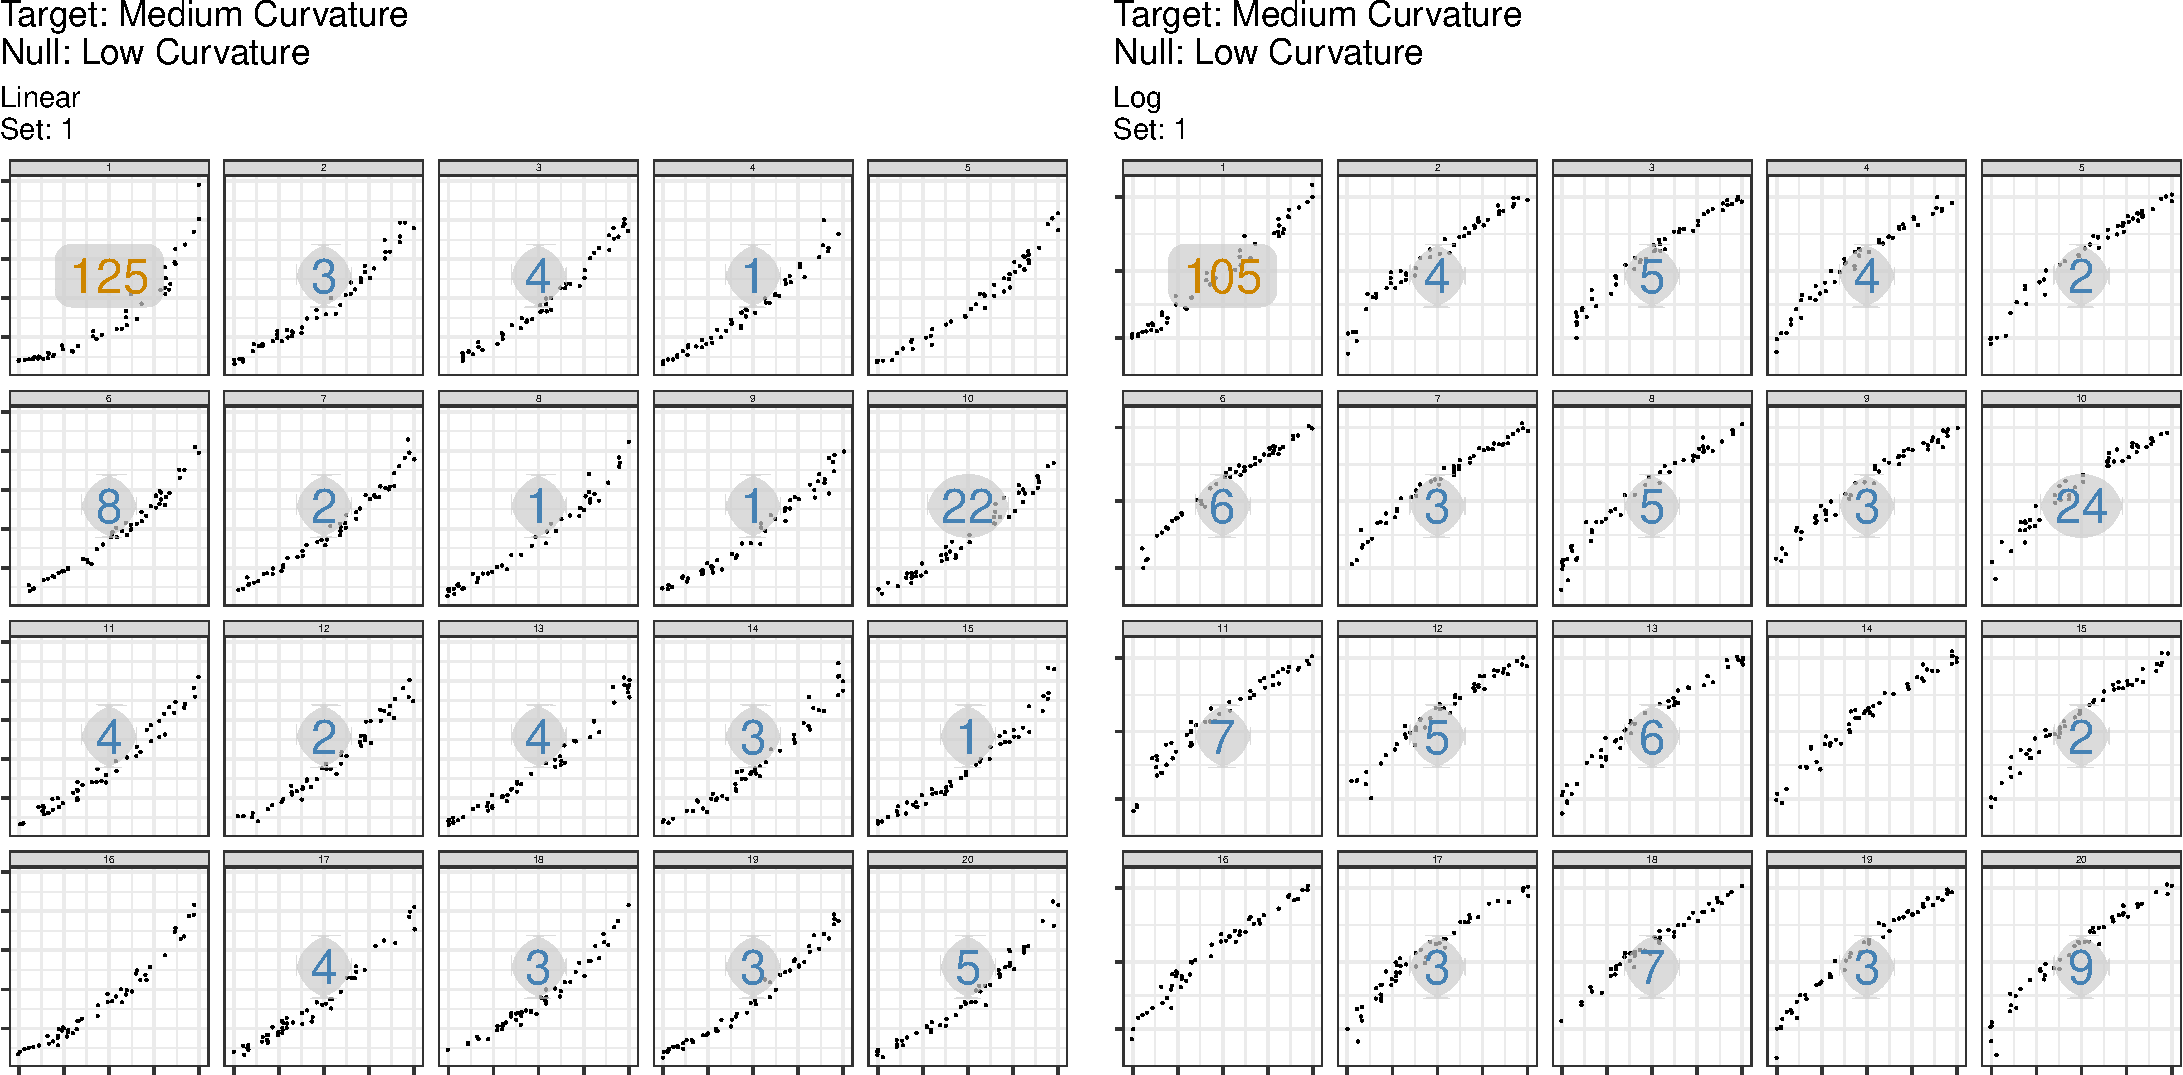
\includegraphics[width=\linewidth,]{appendix-3_files/figure-latex/unnamed-chunk-4-3} \end{center}

\begin{center}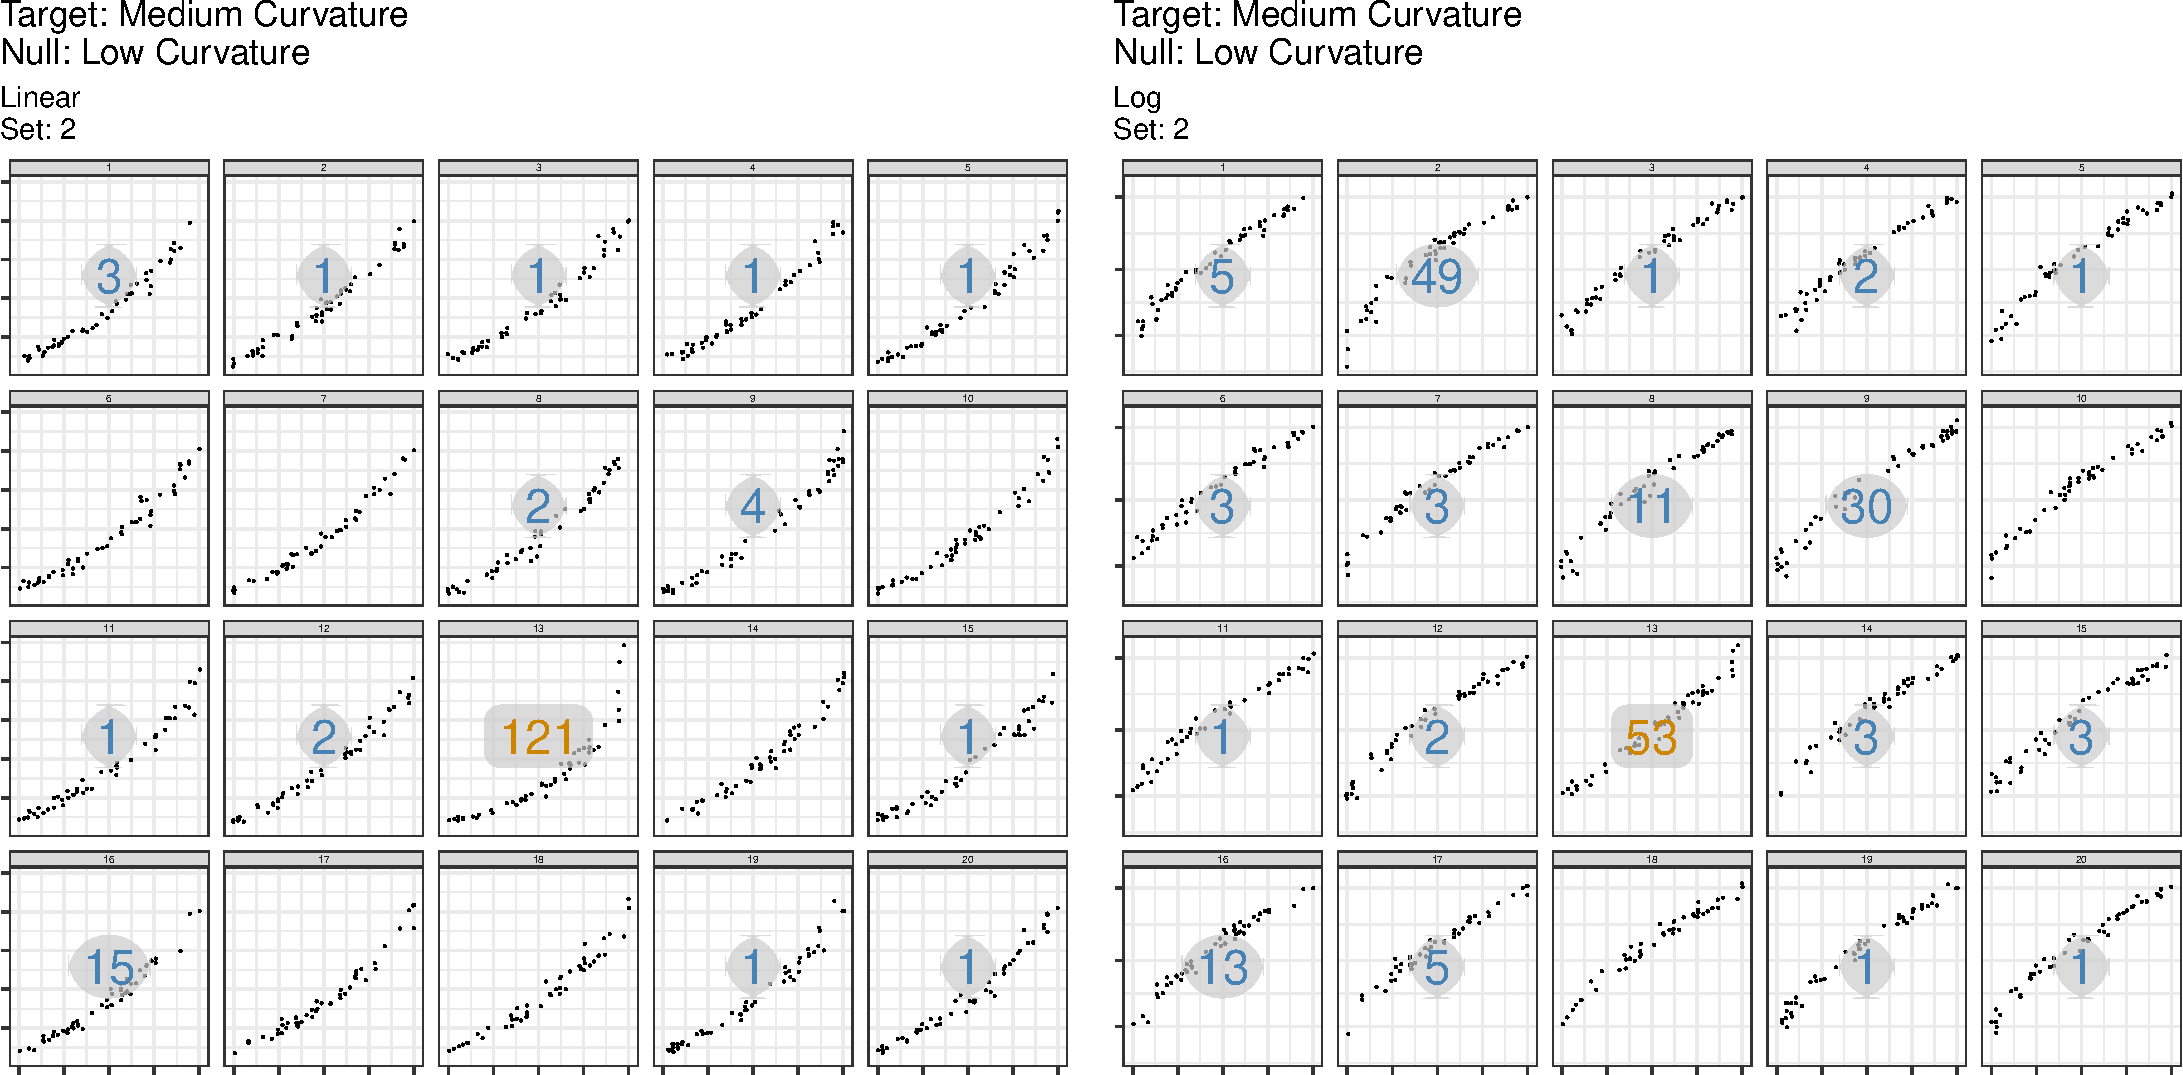
\includegraphics[width=\linewidth,]{appendix-3_files/figure-latex/unnamed-chunk-4-4} \end{center}

\begin{center}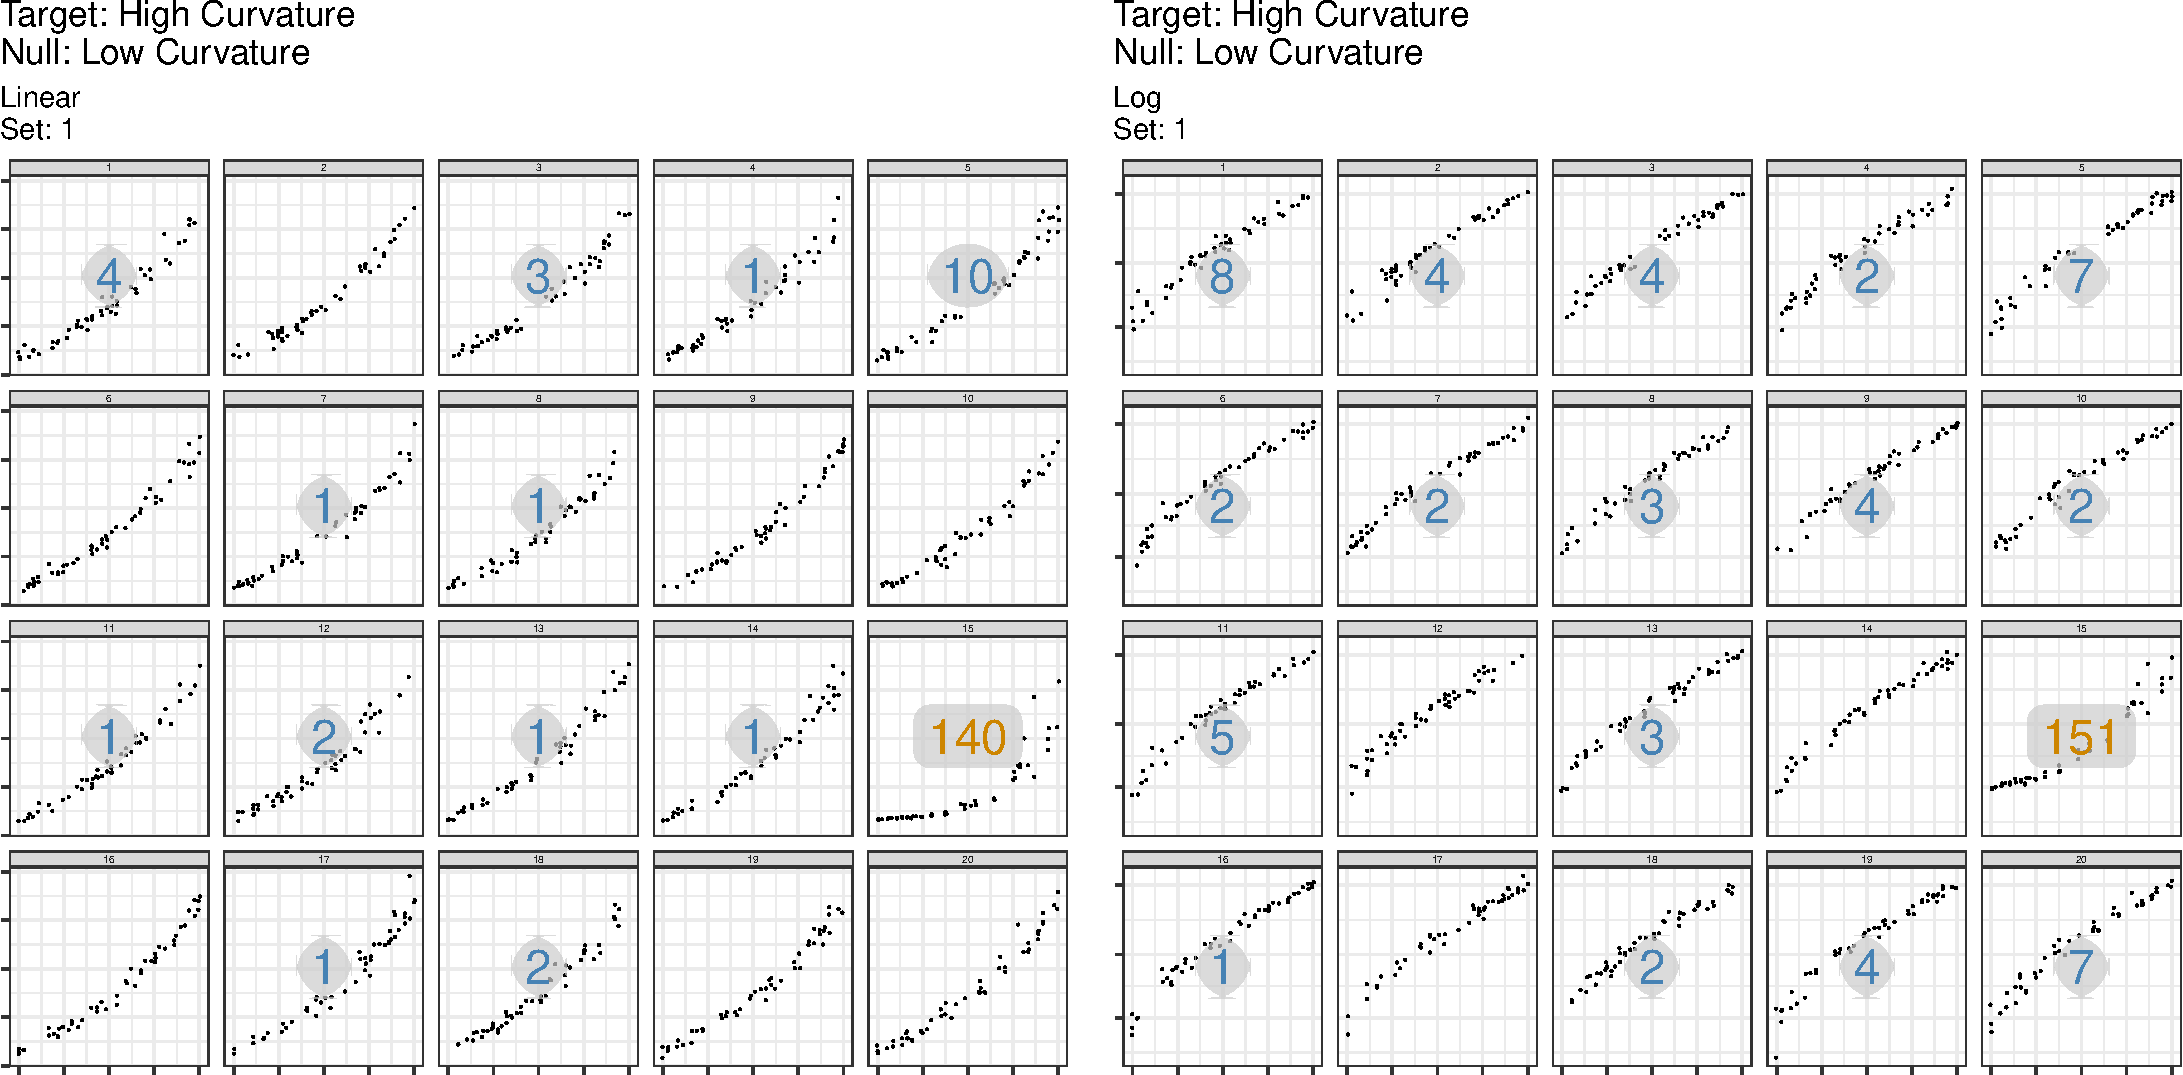
\includegraphics[width=\linewidth,]{appendix-3_files/figure-latex/unnamed-chunk-4-5} \end{center}

\begin{center}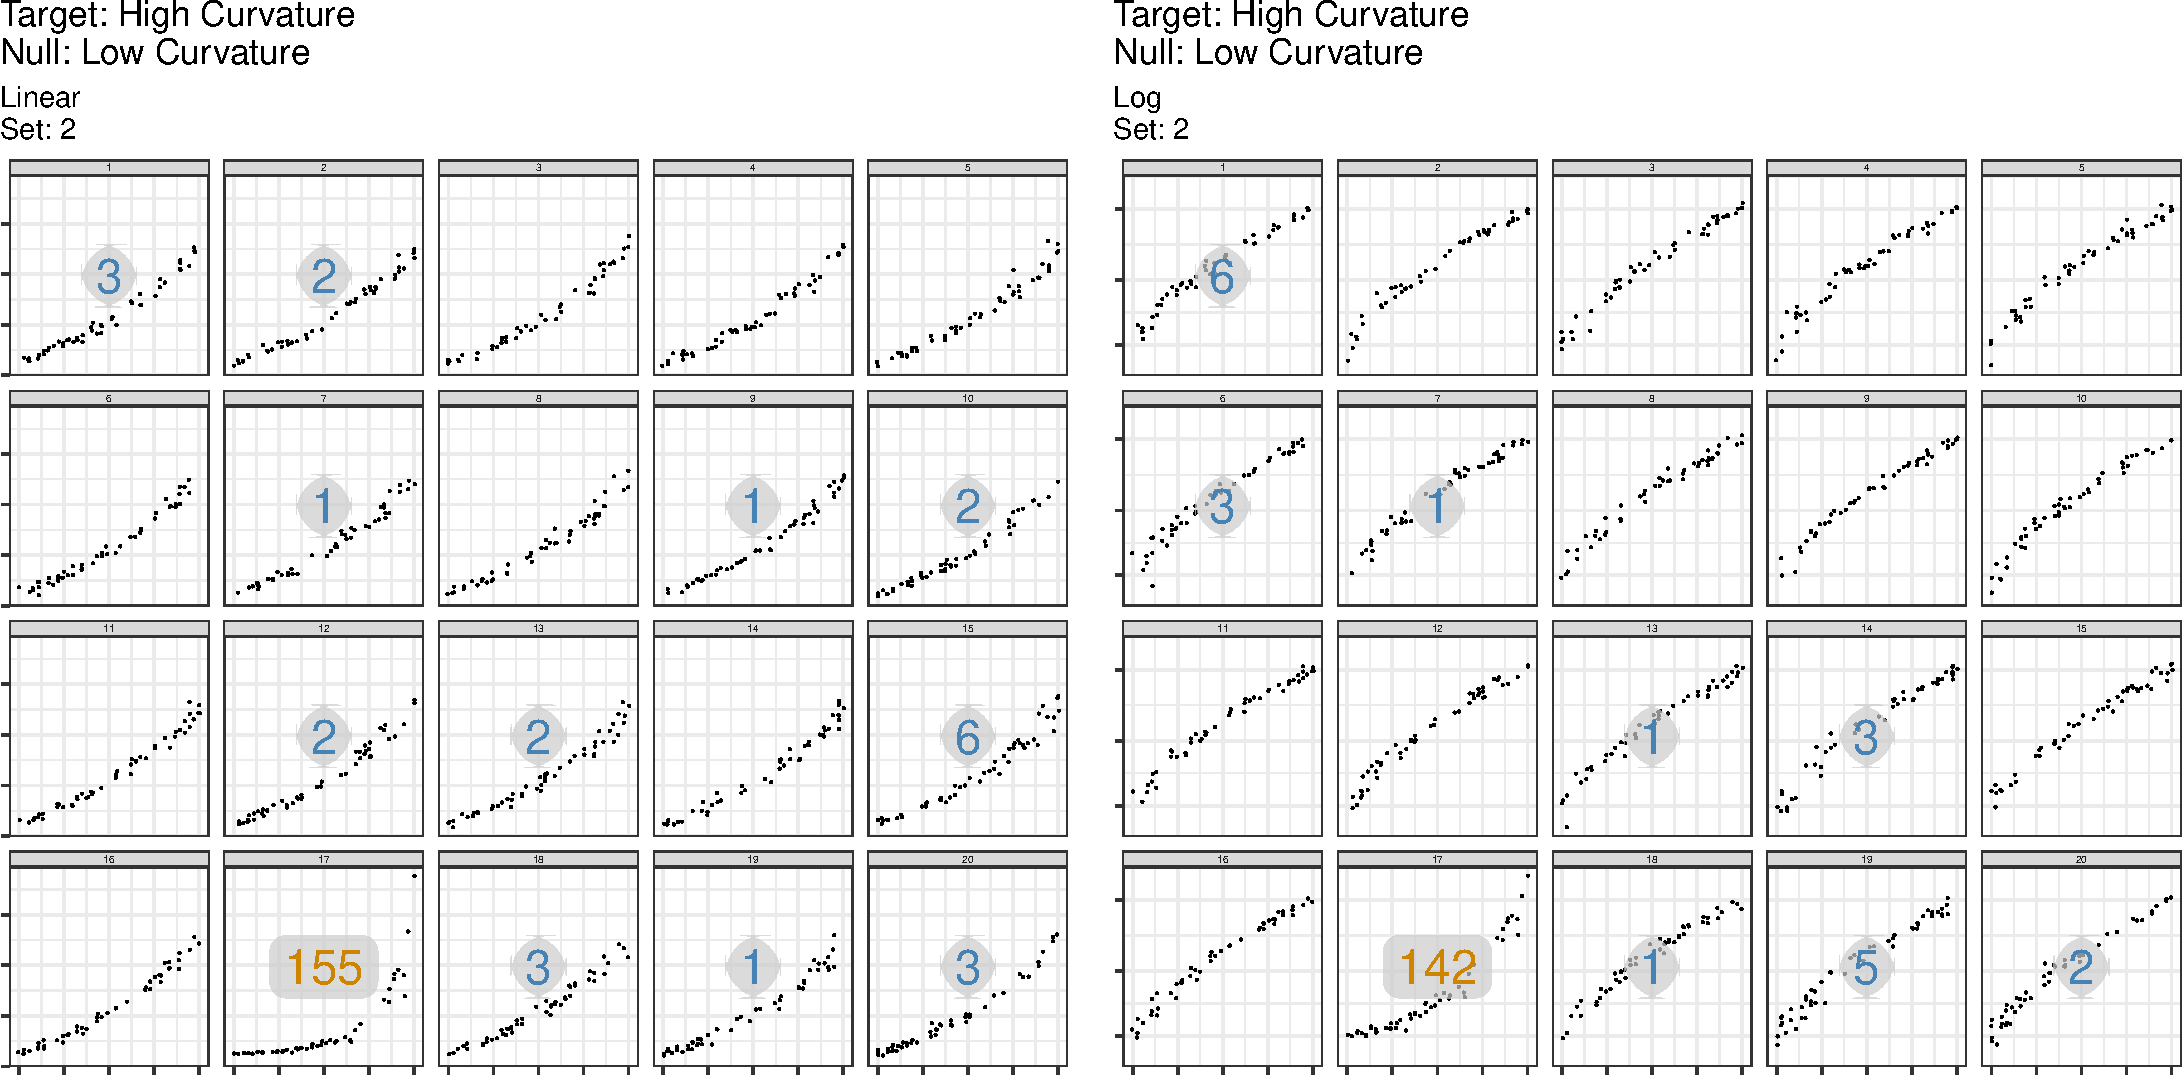
\includegraphics[width=\linewidth,]{appendix-3_files/figure-latex/unnamed-chunk-4-6} \end{center}

\subsection{Medium Curvature Null
Background}\label{medium-curvature-null-background}

\begin{center}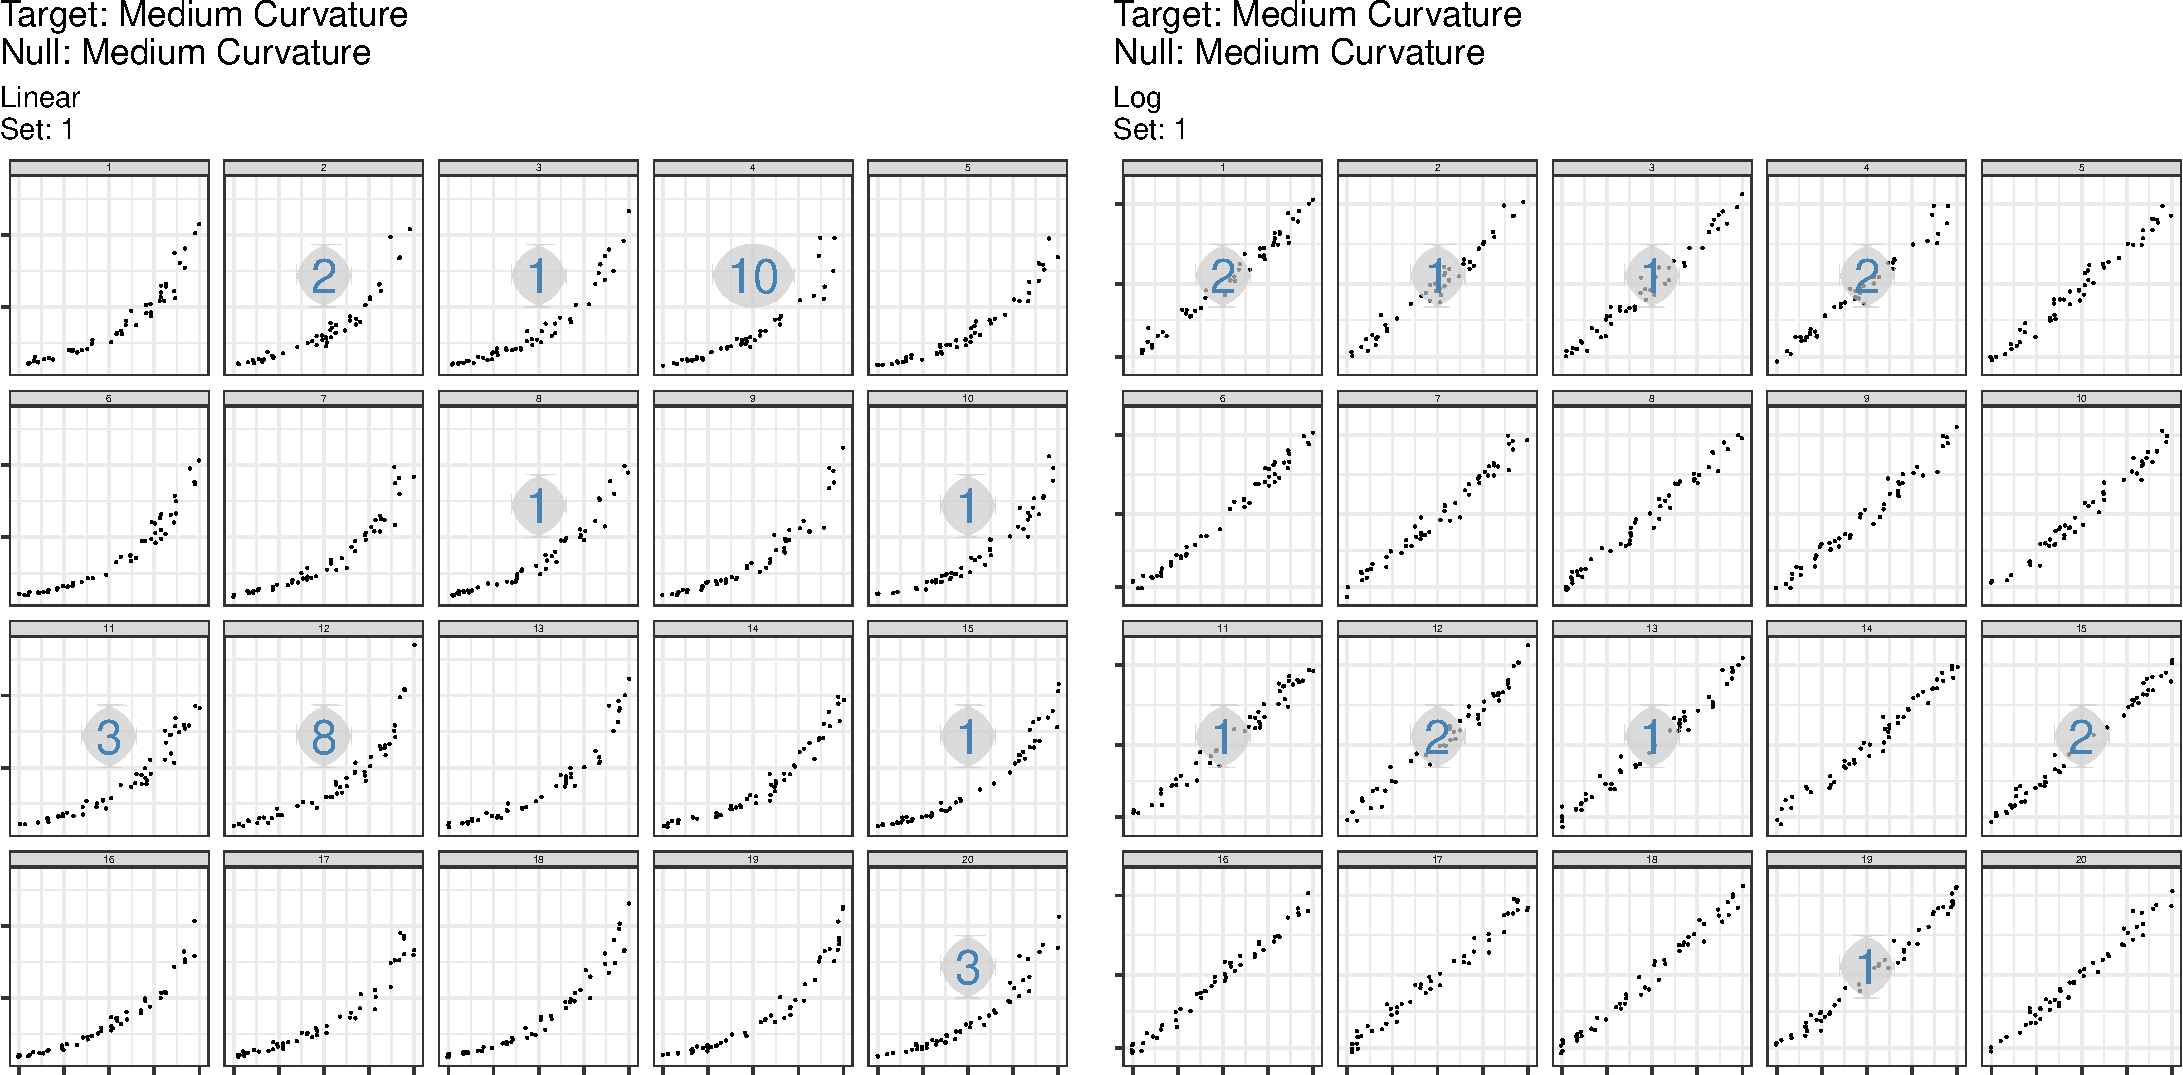
\includegraphics[width=\linewidth,]{appendix-3_files/figure-latex/unnamed-chunk-5-1} \end{center}

\begin{center}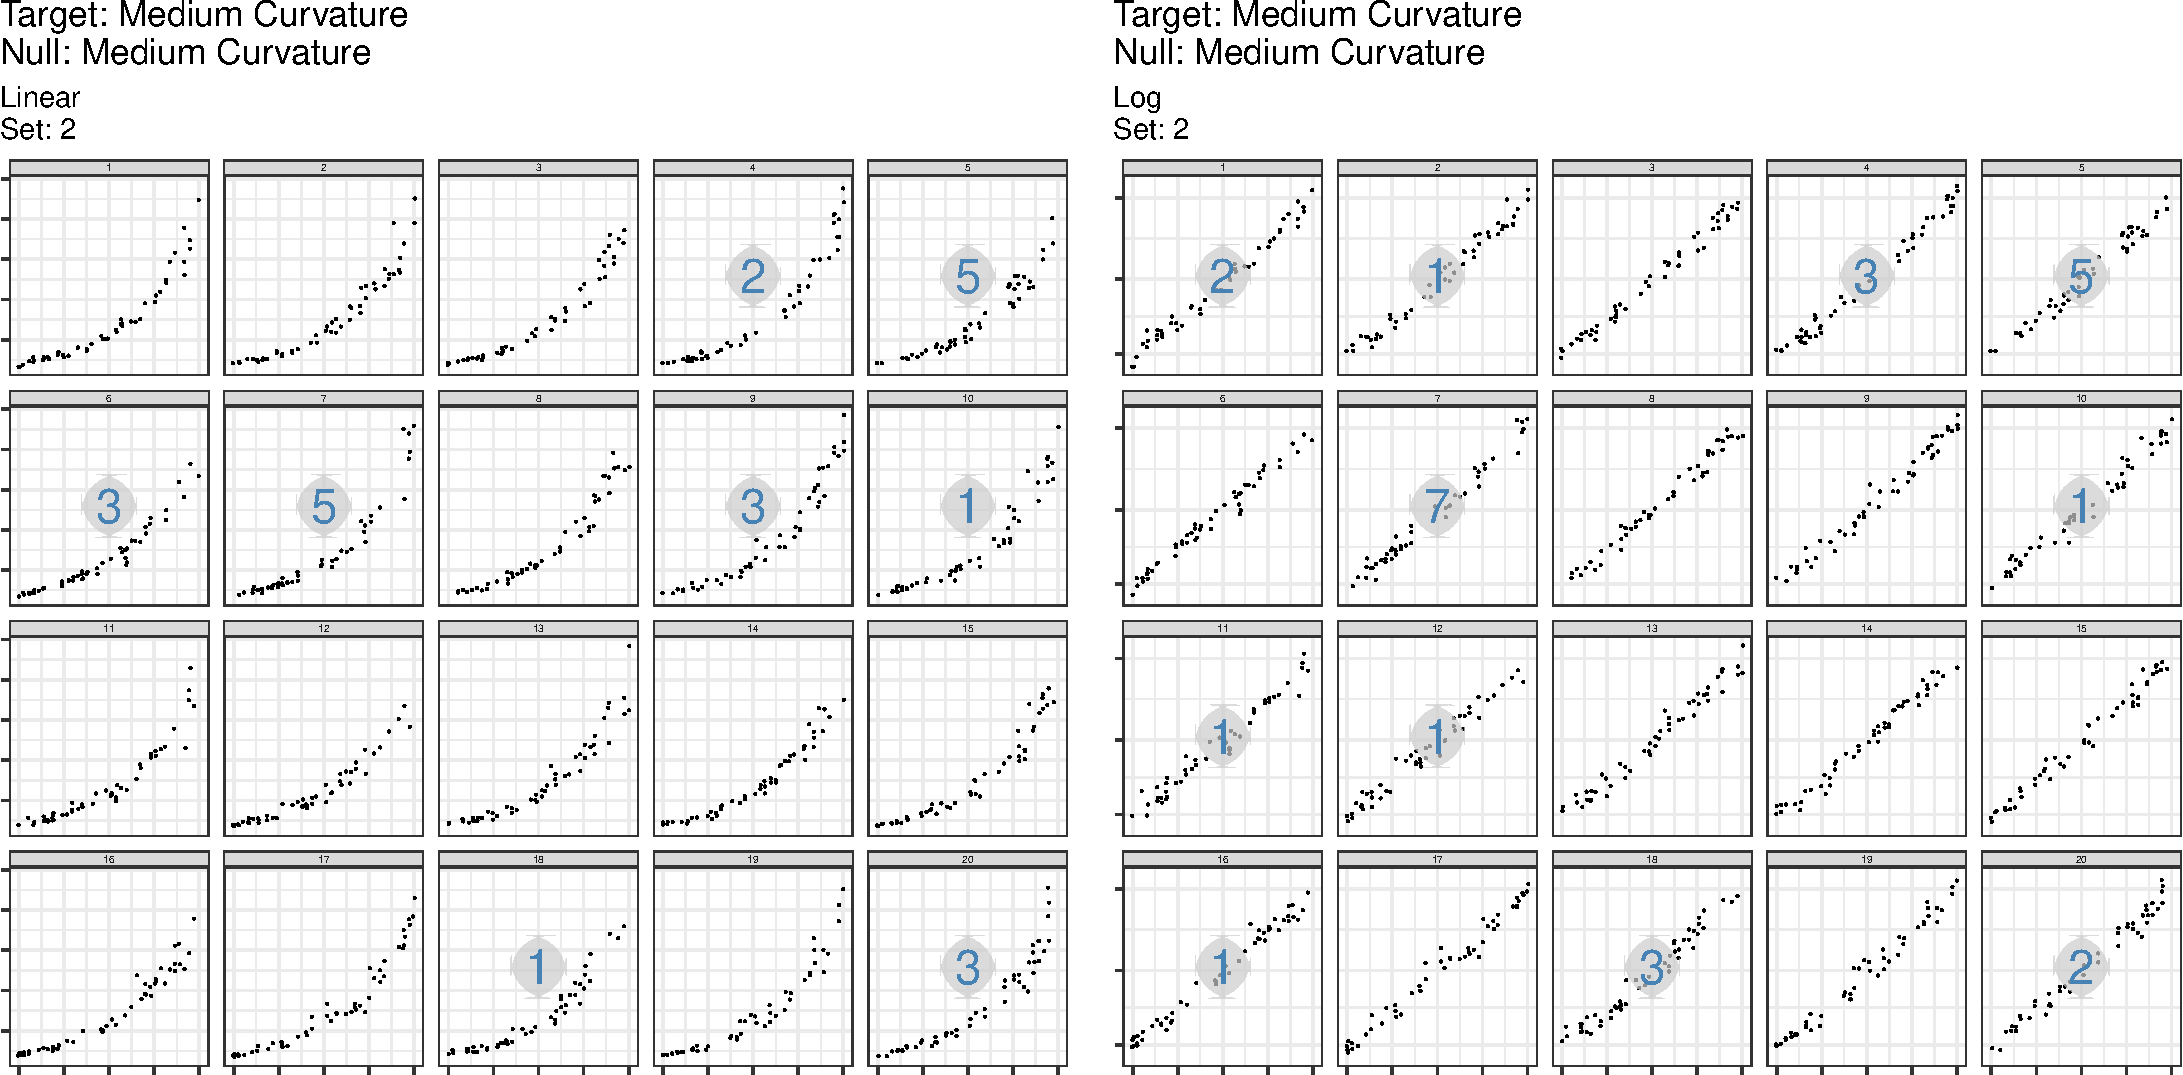
\includegraphics[width=\linewidth,]{appendix-3_files/figure-latex/unnamed-chunk-5-2} \end{center}

\begin{center}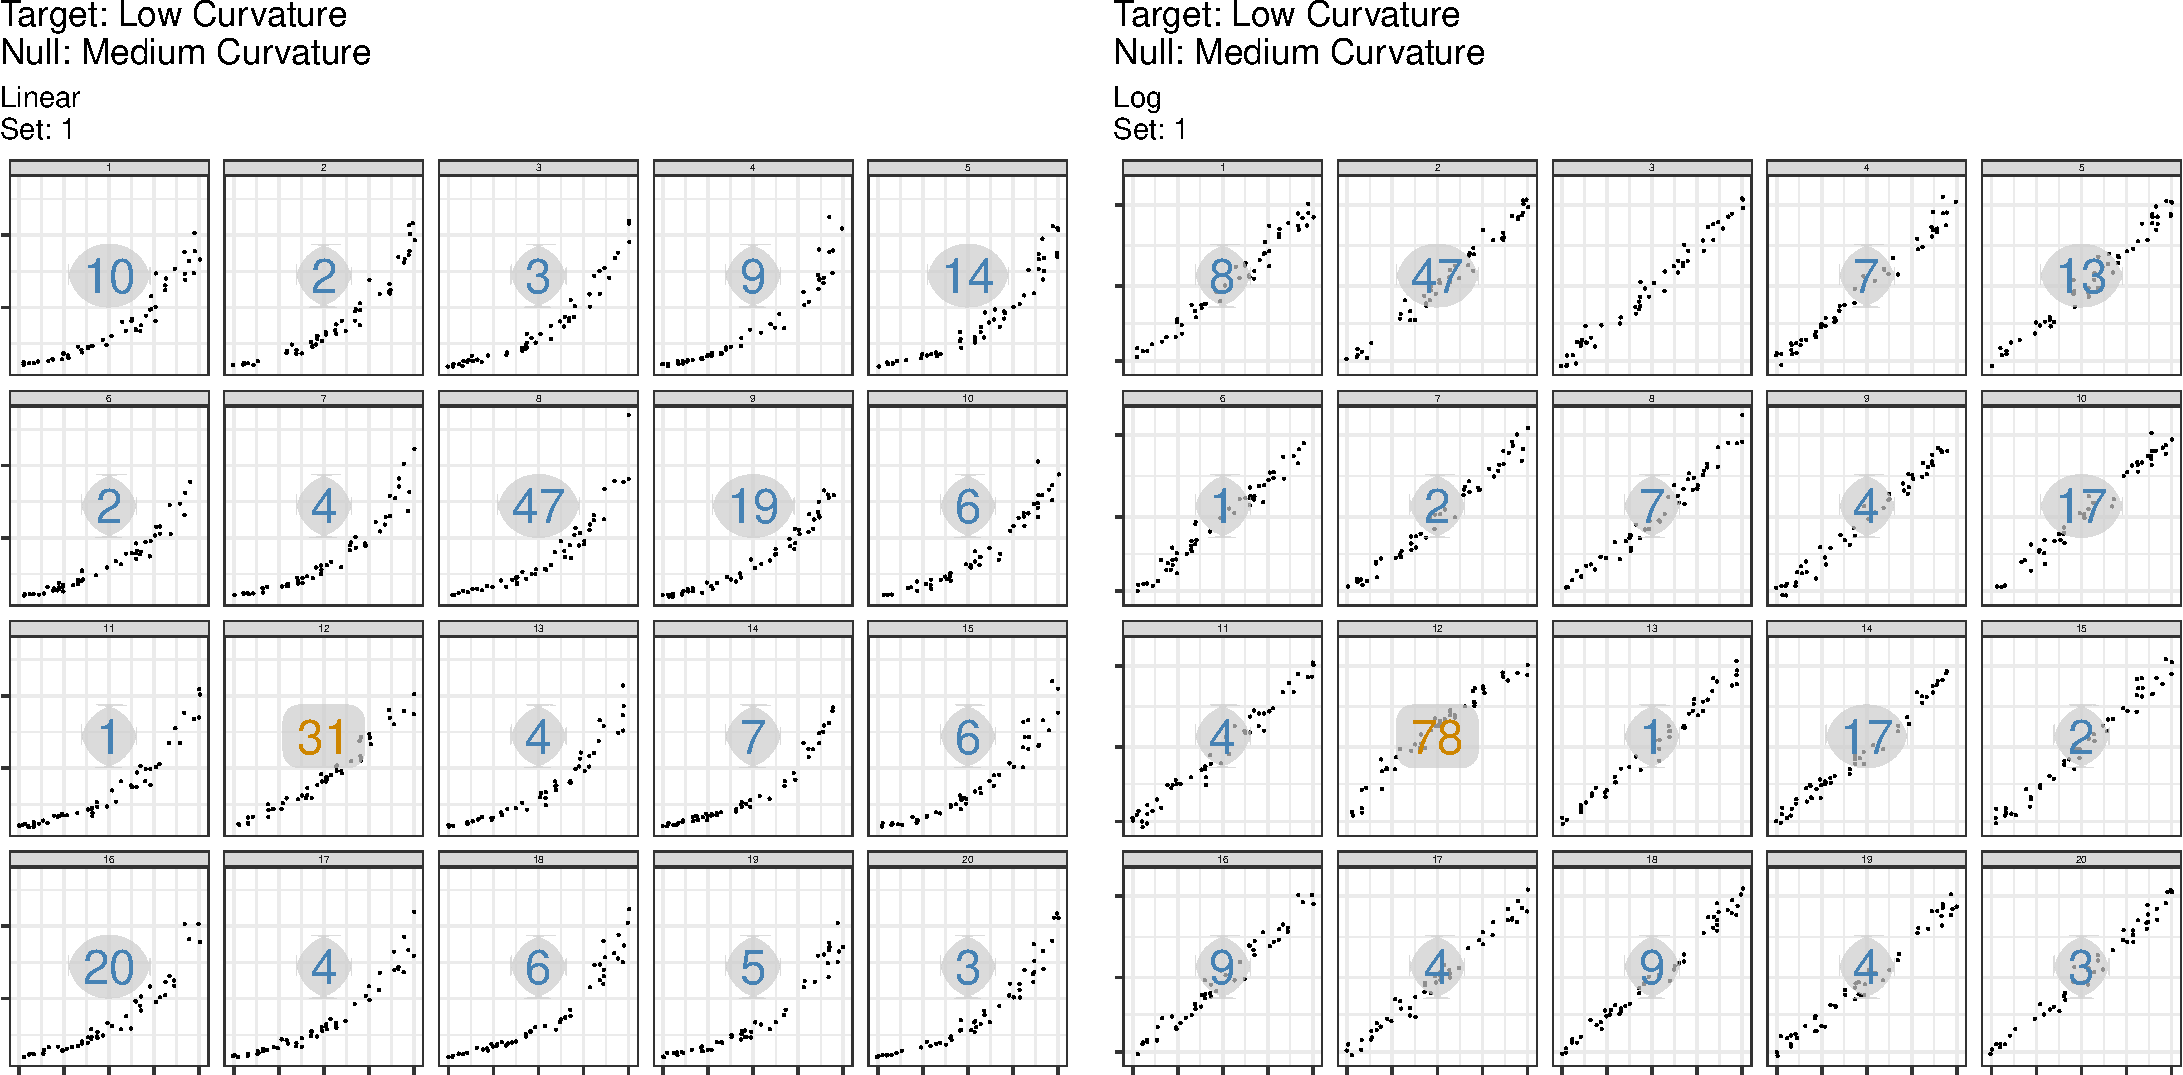
\includegraphics[width=\linewidth,]{appendix-3_files/figure-latex/unnamed-chunk-5-3} \end{center}

\begin{center}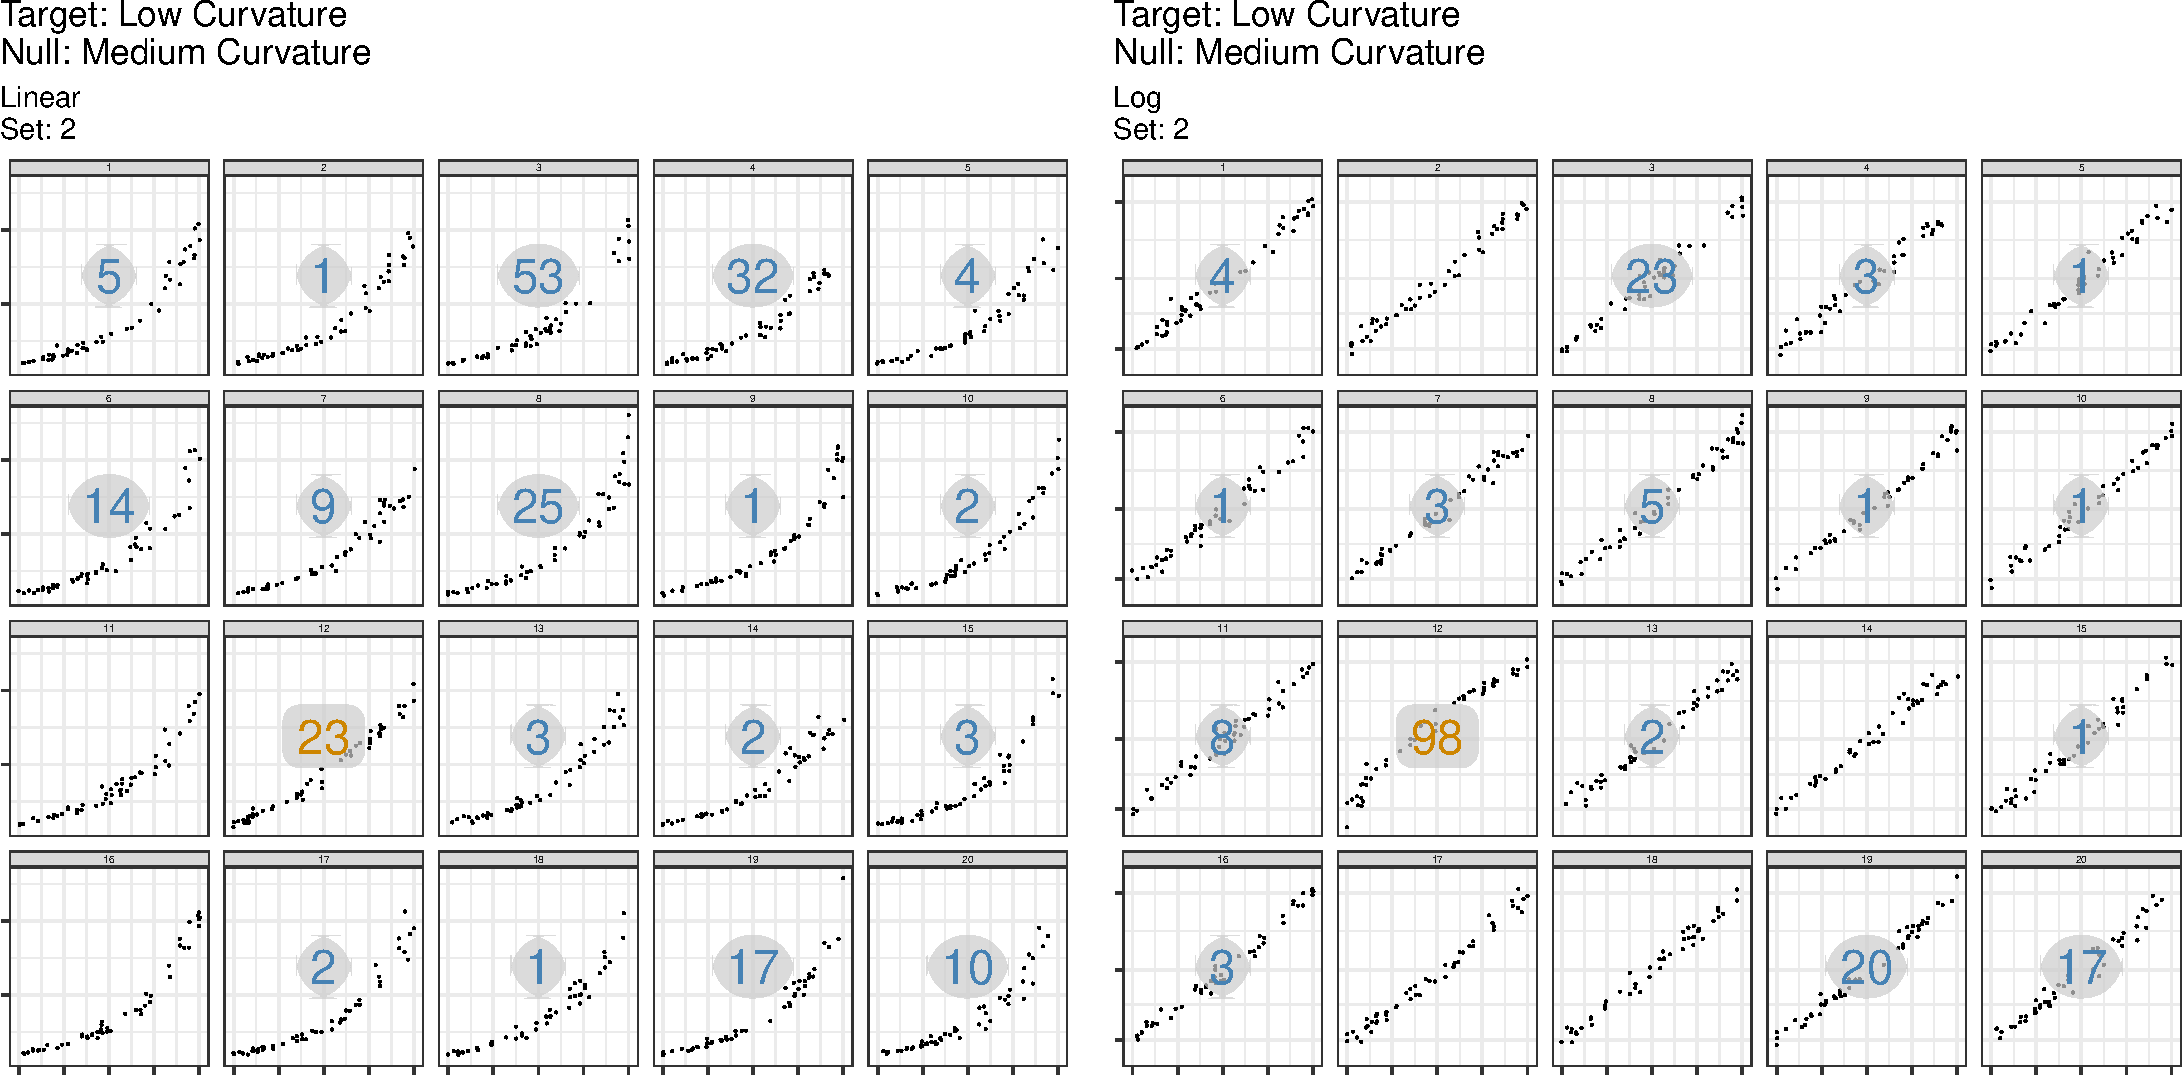
\includegraphics[width=\linewidth,]{appendix-3_files/figure-latex/unnamed-chunk-5-4} \end{center}

\begin{center}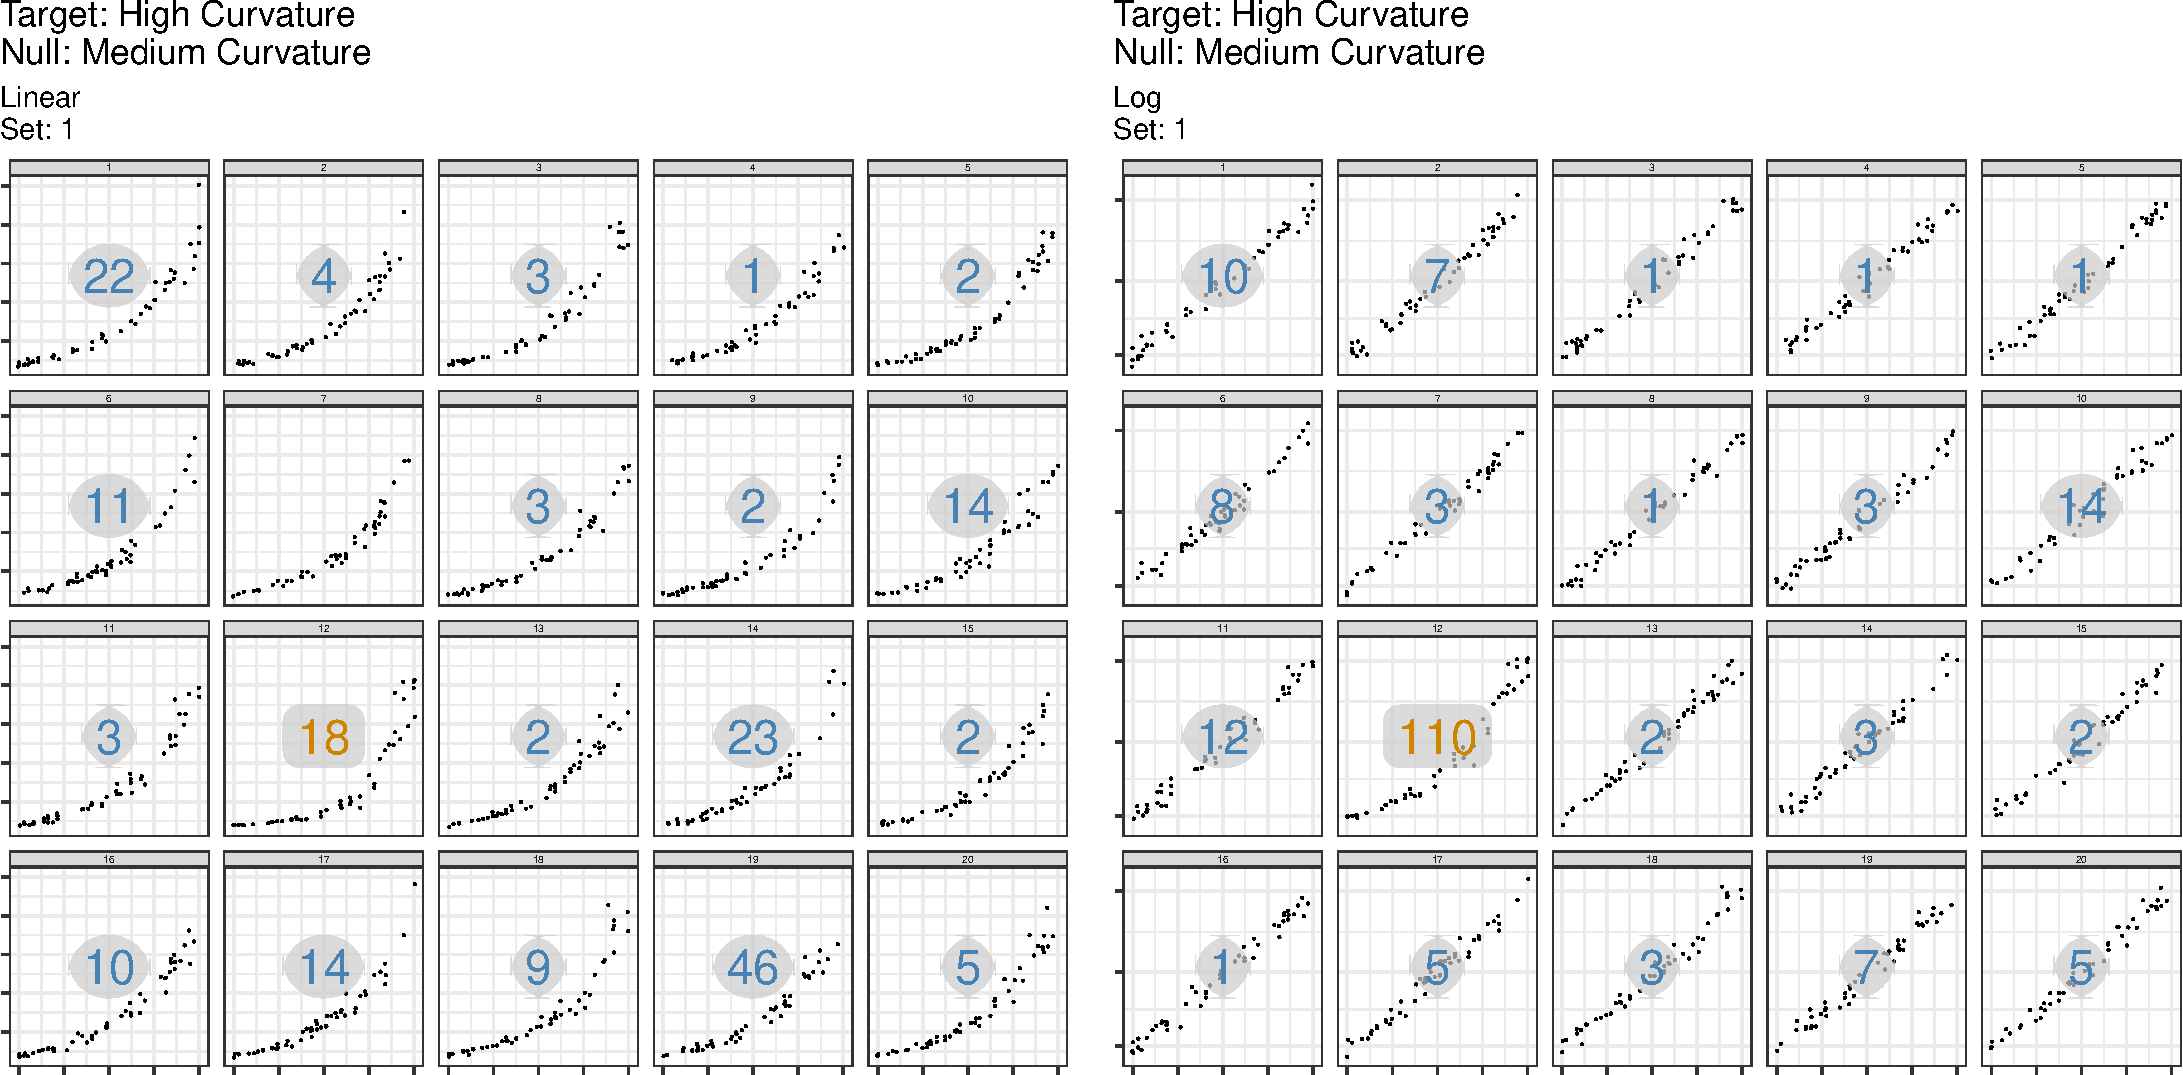
\includegraphics[width=\linewidth,]{appendix-3_files/figure-latex/unnamed-chunk-5-5} \end{center}

\begin{center}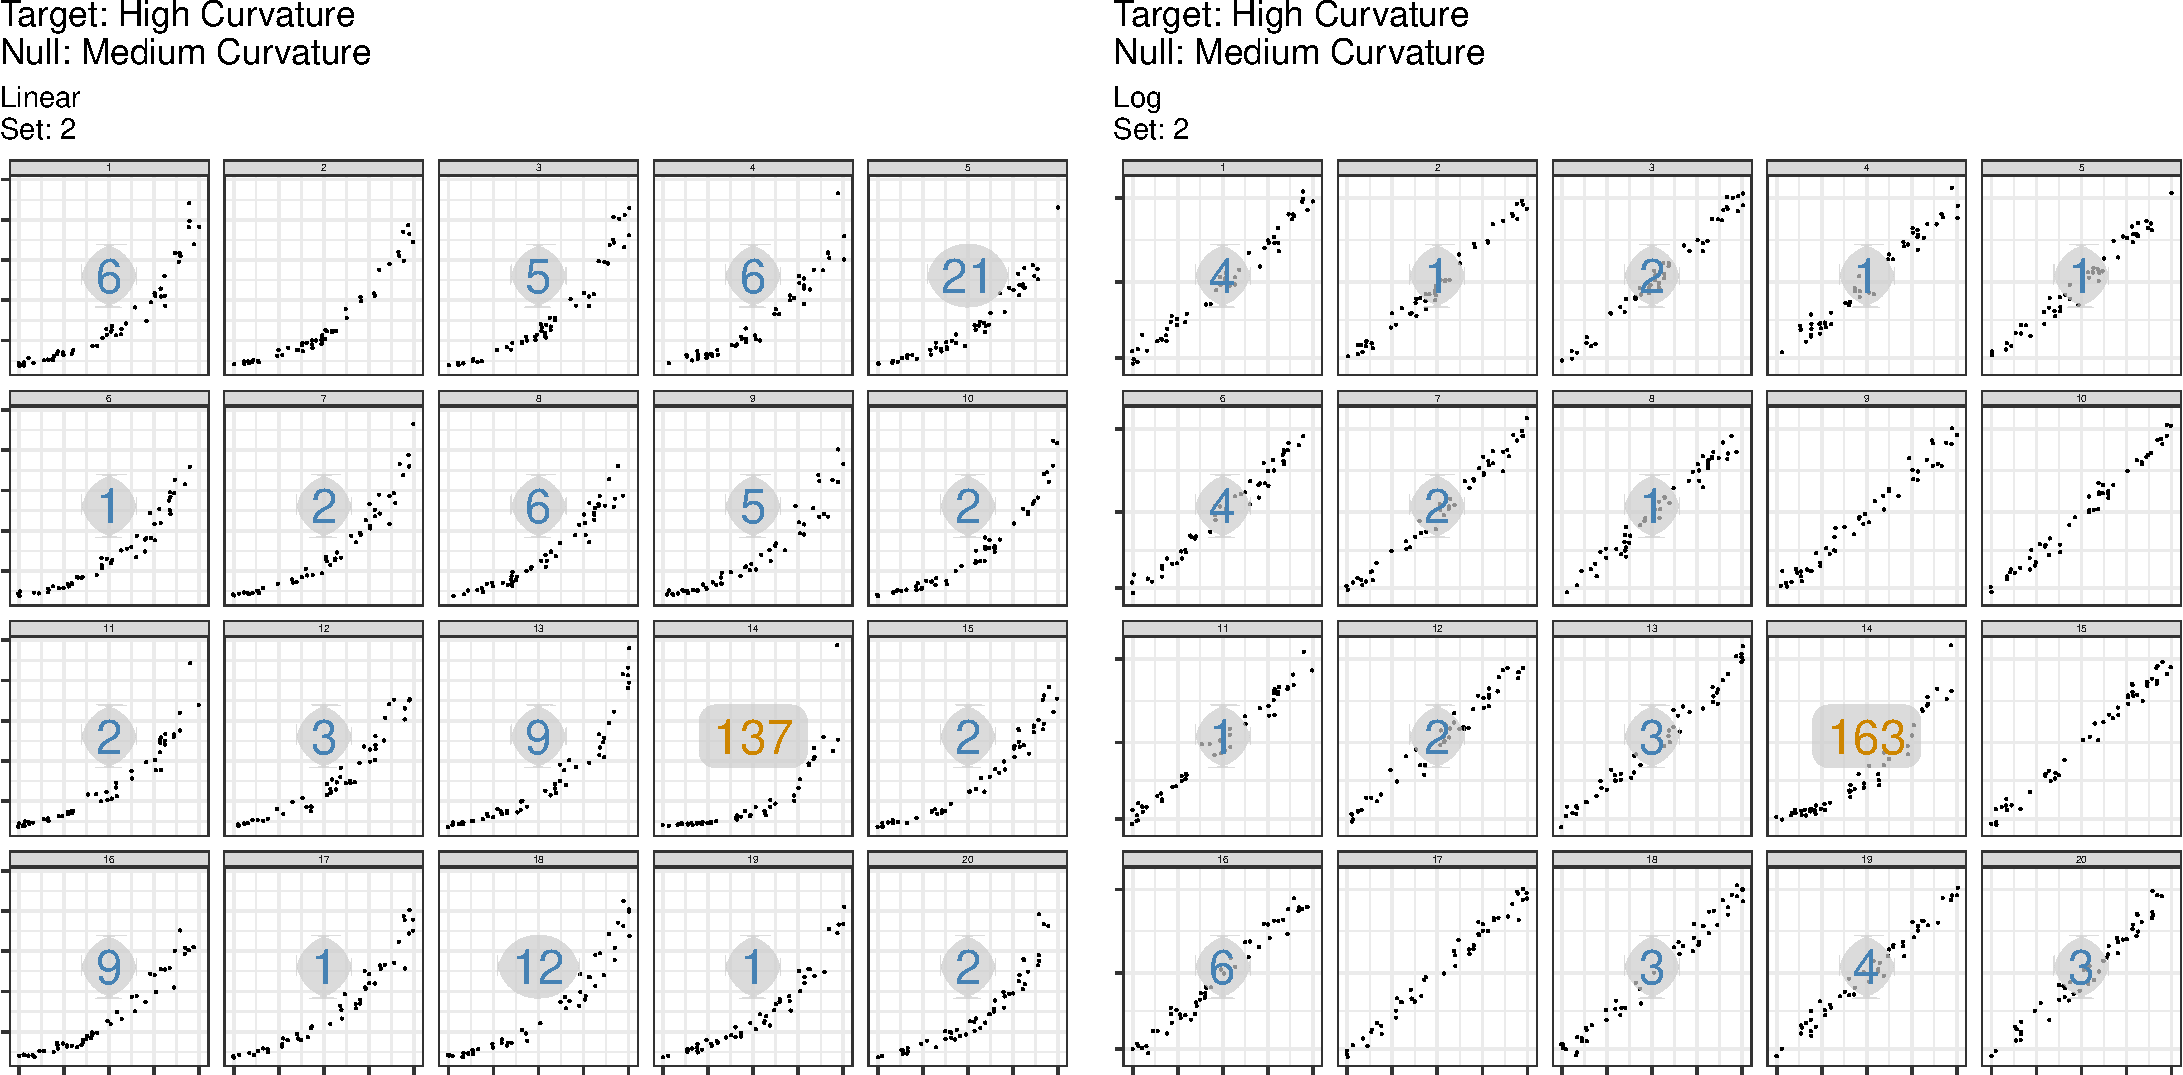
\includegraphics[width=\linewidth,]{appendix-3_files/figure-latex/unnamed-chunk-5-6} \end{center}

\subsection{High Curvature Null
Background}\label{high-curvature-null-background}

\begin{center}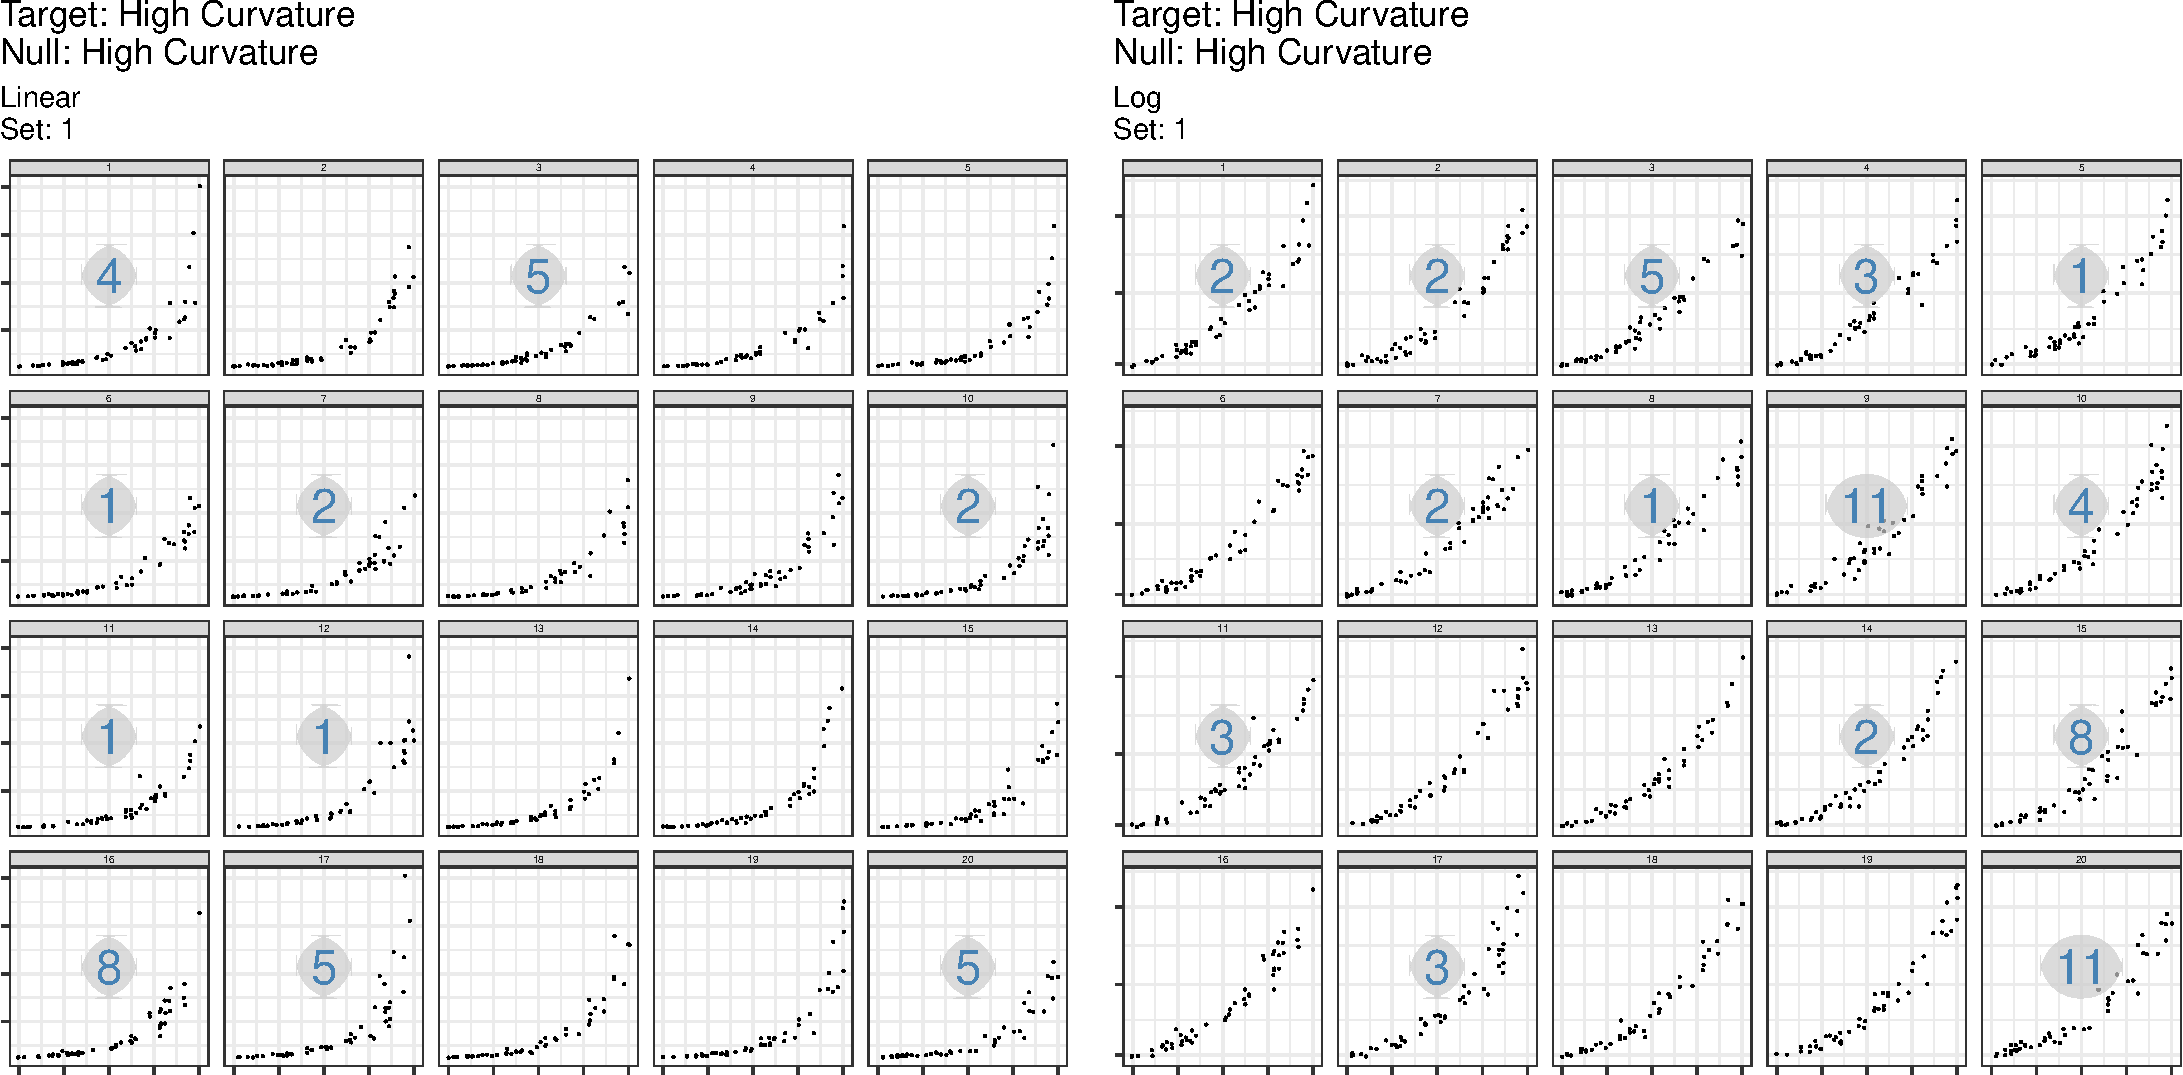
\includegraphics[width=\linewidth,]{appendix-3_files/figure-latex/unnamed-chunk-6-1} \end{center}

\begin{center}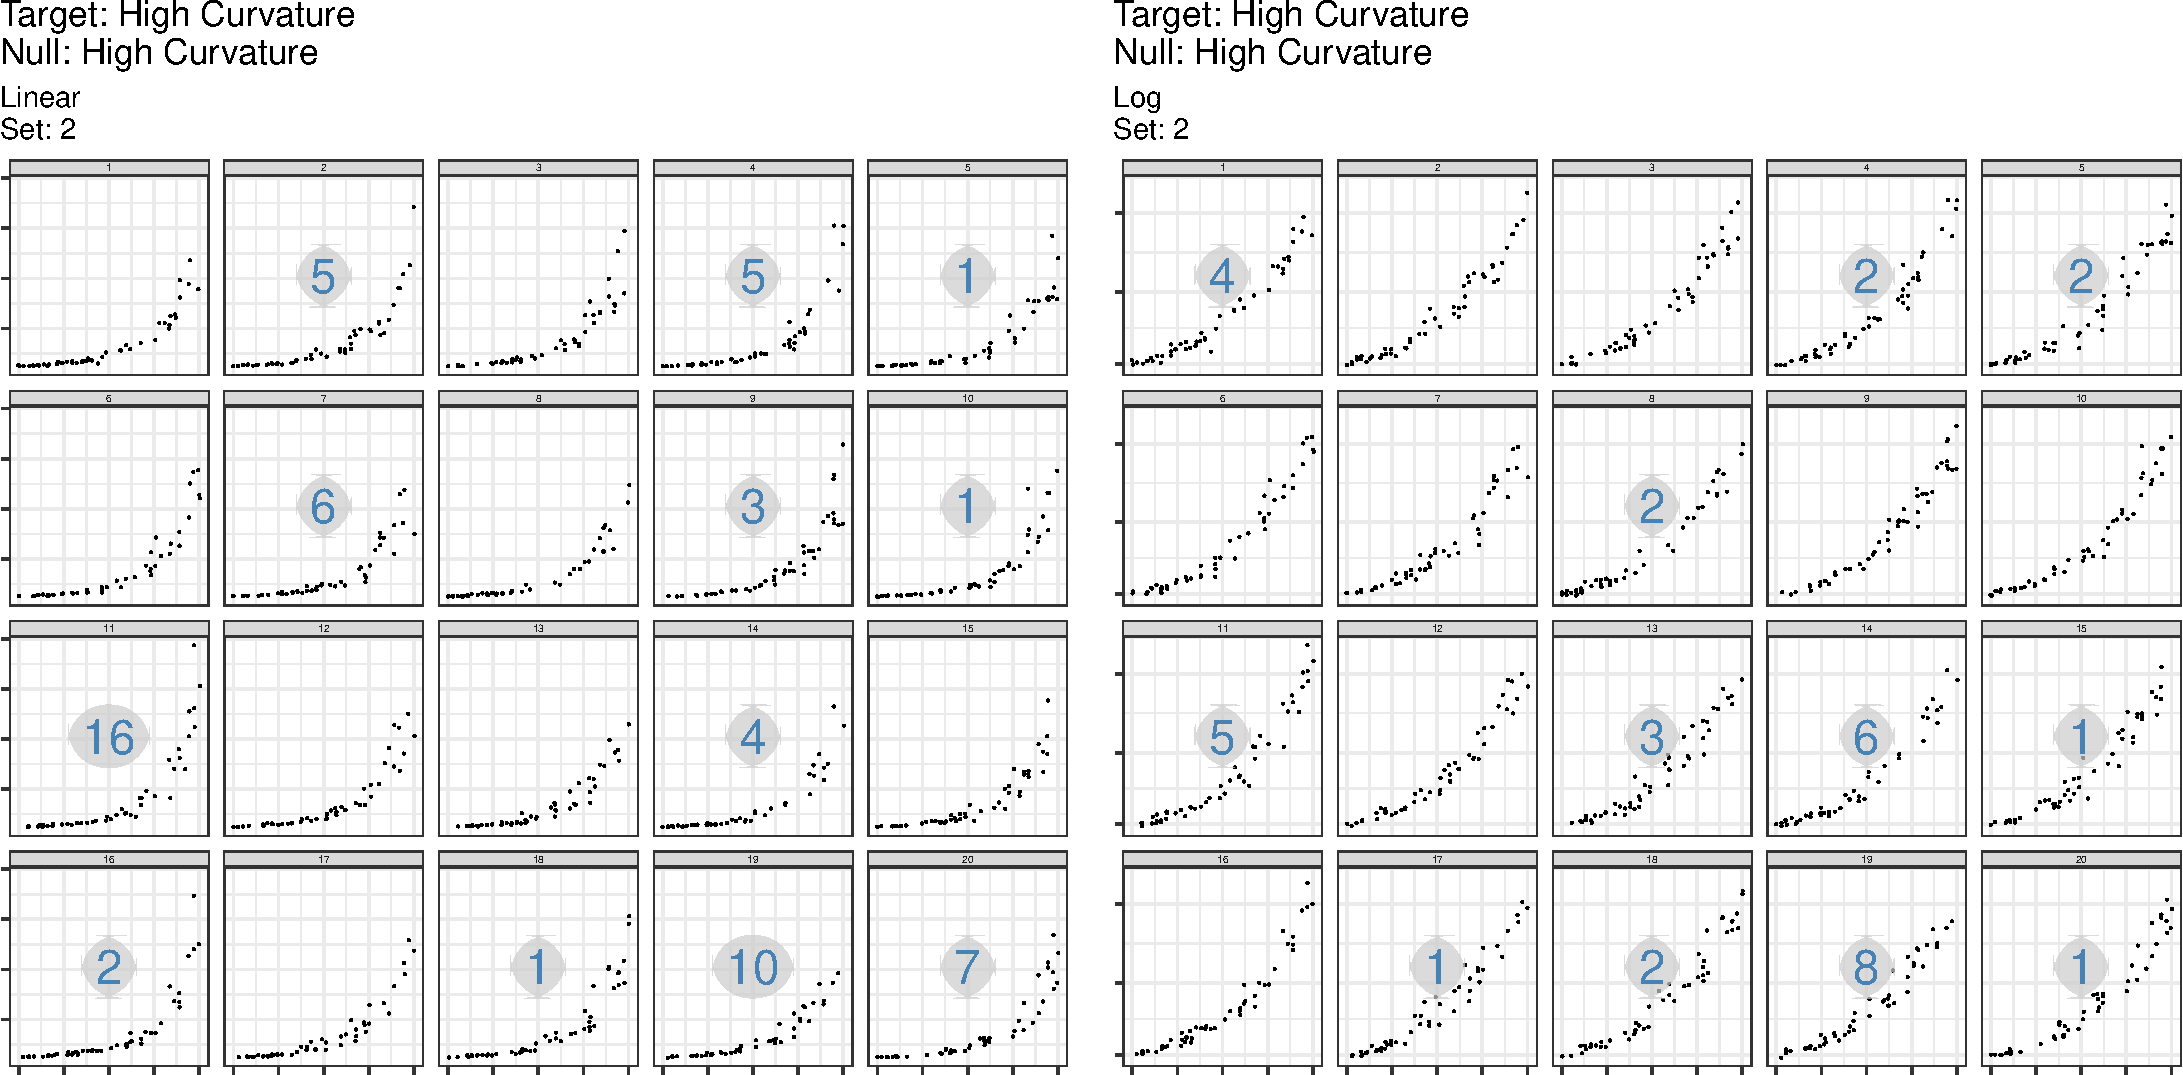
\includegraphics[width=\linewidth,]{appendix-3_files/figure-latex/unnamed-chunk-6-2} \end{center}

\begin{center}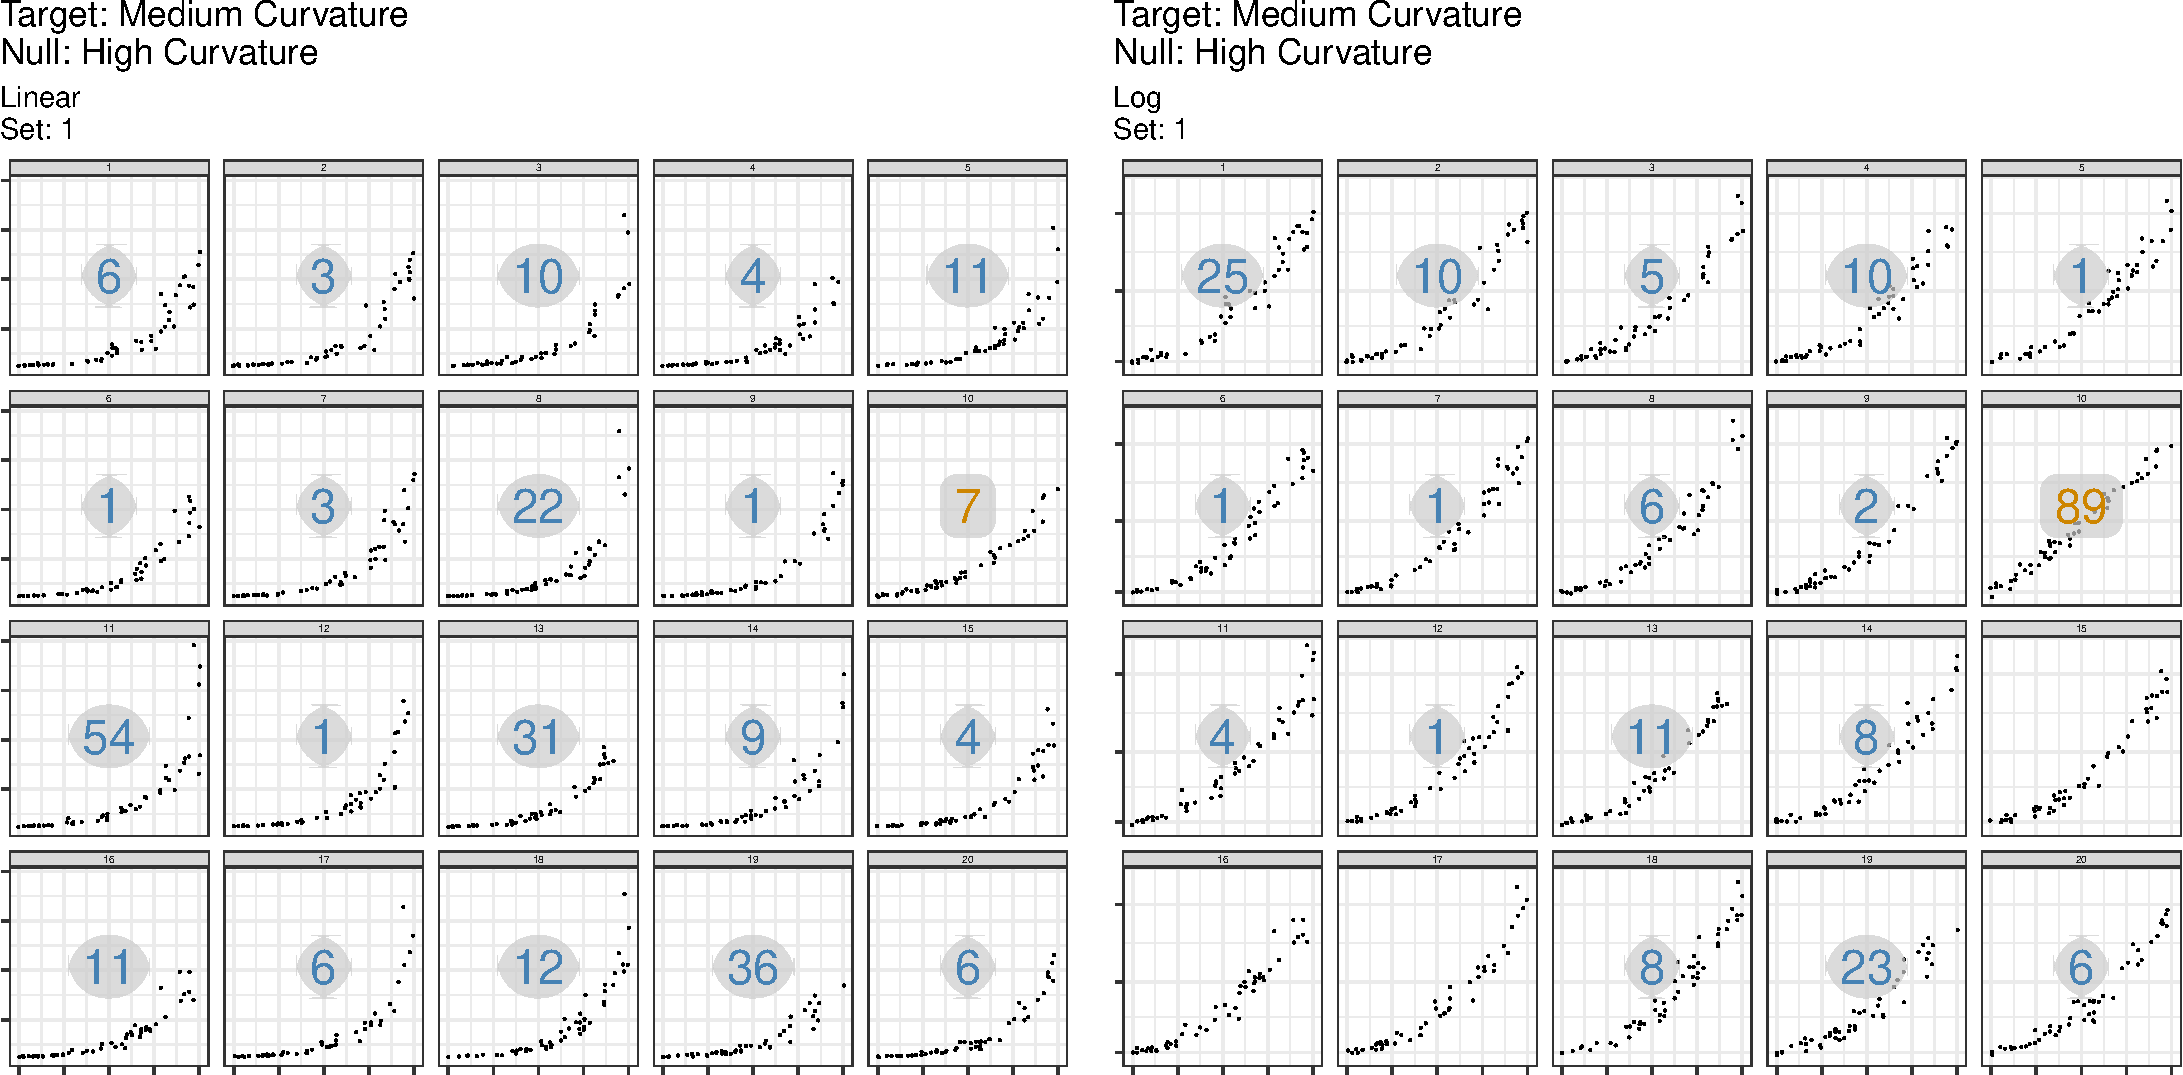
\includegraphics[width=\linewidth,]{appendix-3_files/figure-latex/unnamed-chunk-6-3} \end{center}

\begin{center}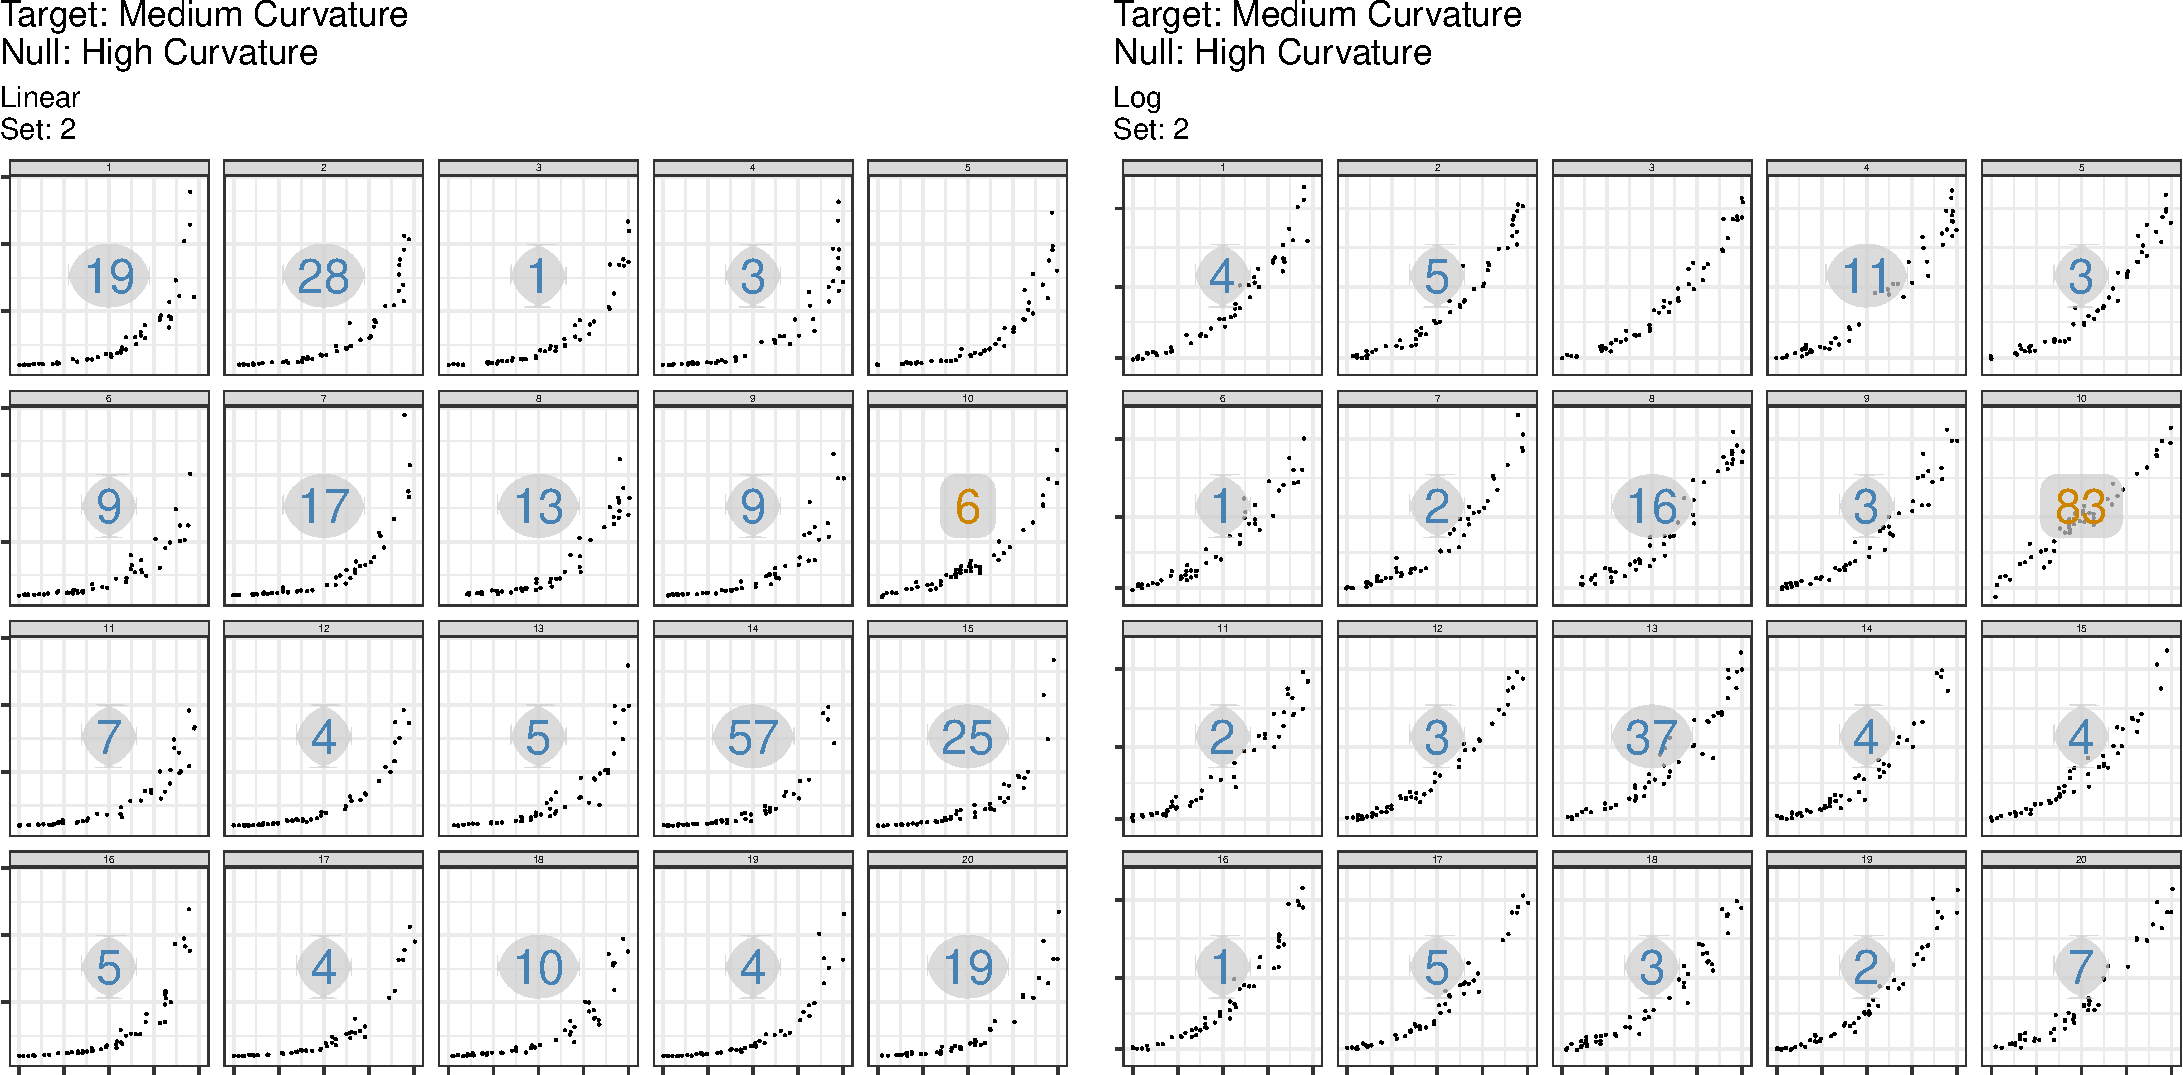
\includegraphics[width=\linewidth,]{appendix-3_files/figure-latex/unnamed-chunk-6-4} \end{center}

\begin{center}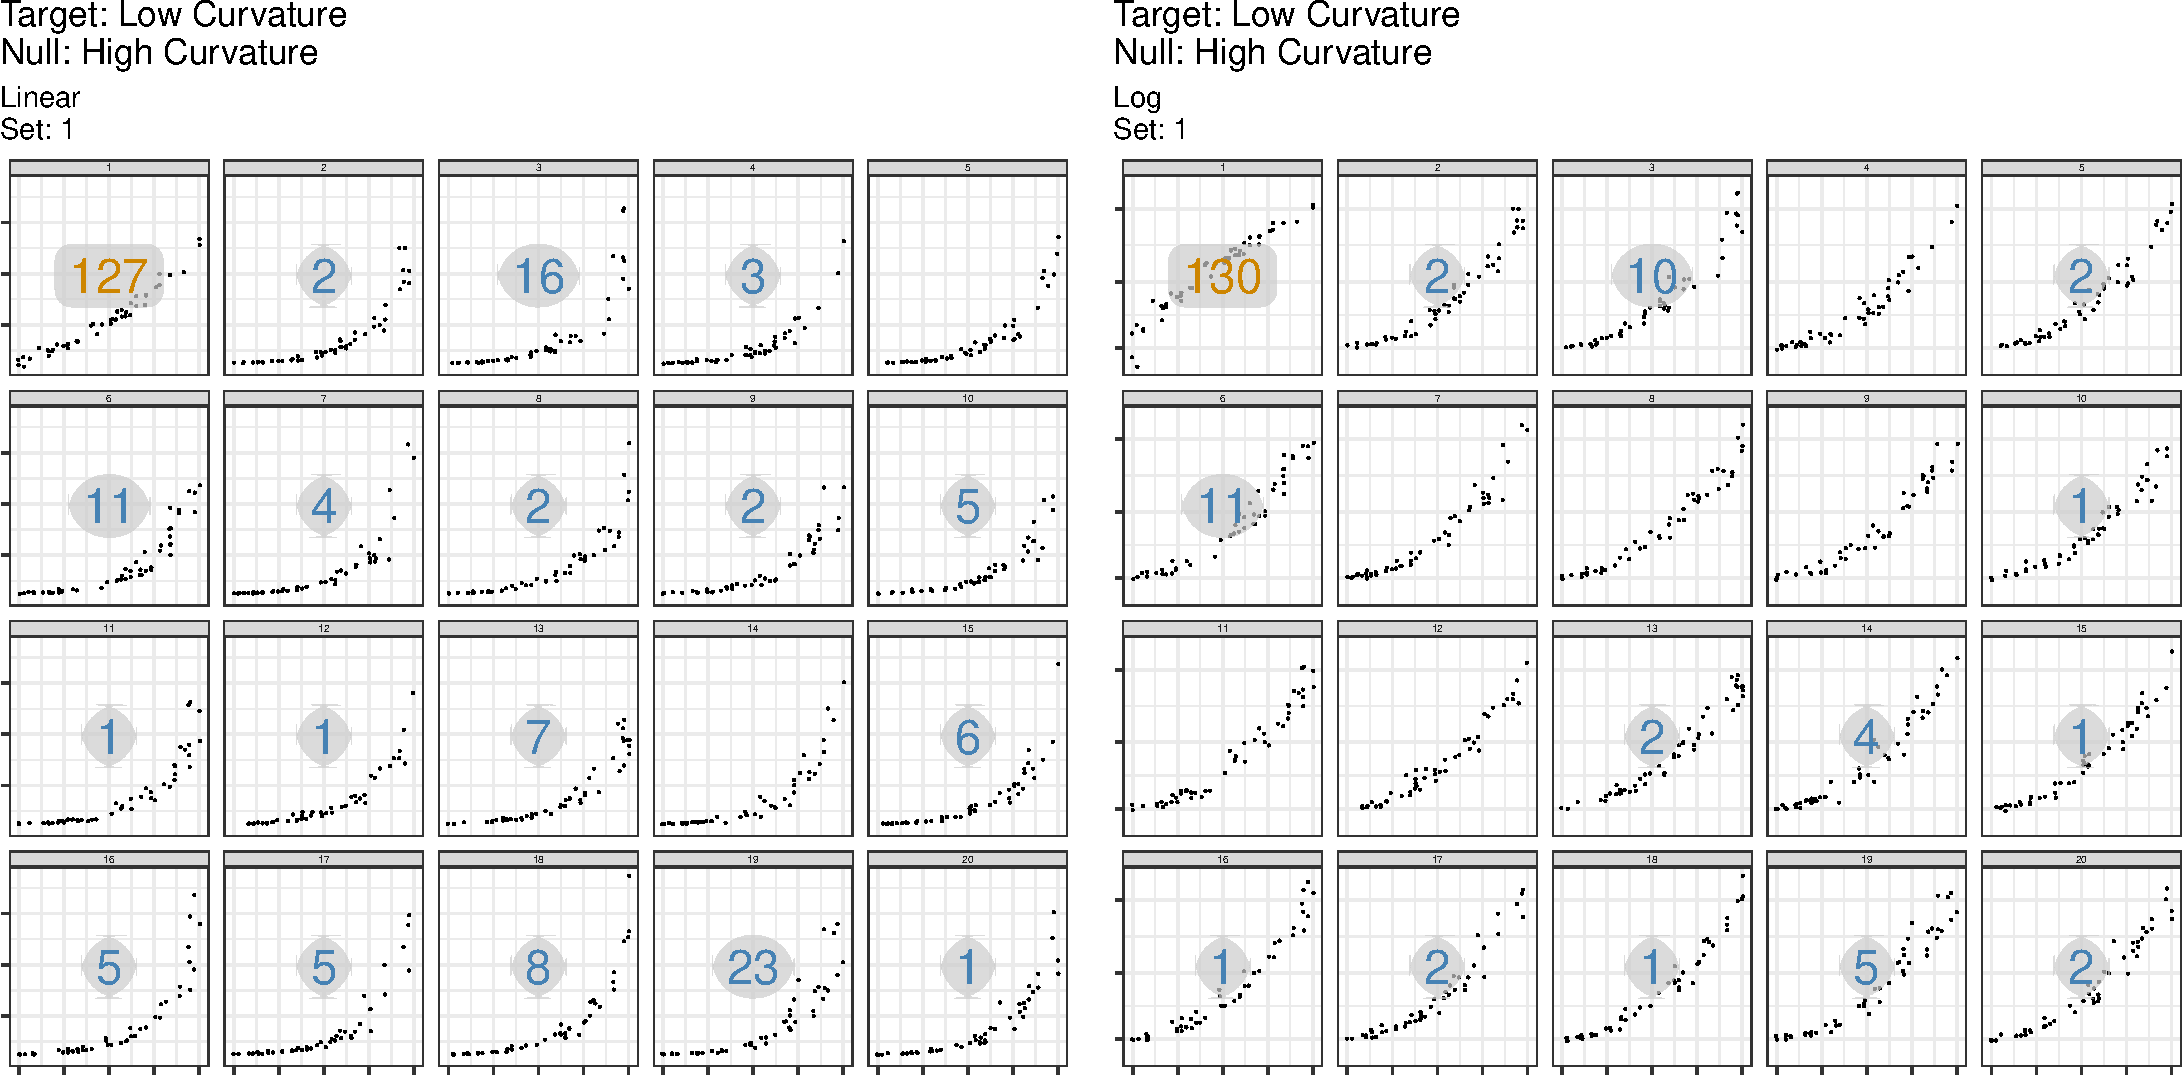
\includegraphics[width=\linewidth,]{appendix-3_files/figure-latex/unnamed-chunk-6-5} \end{center}

\begin{center}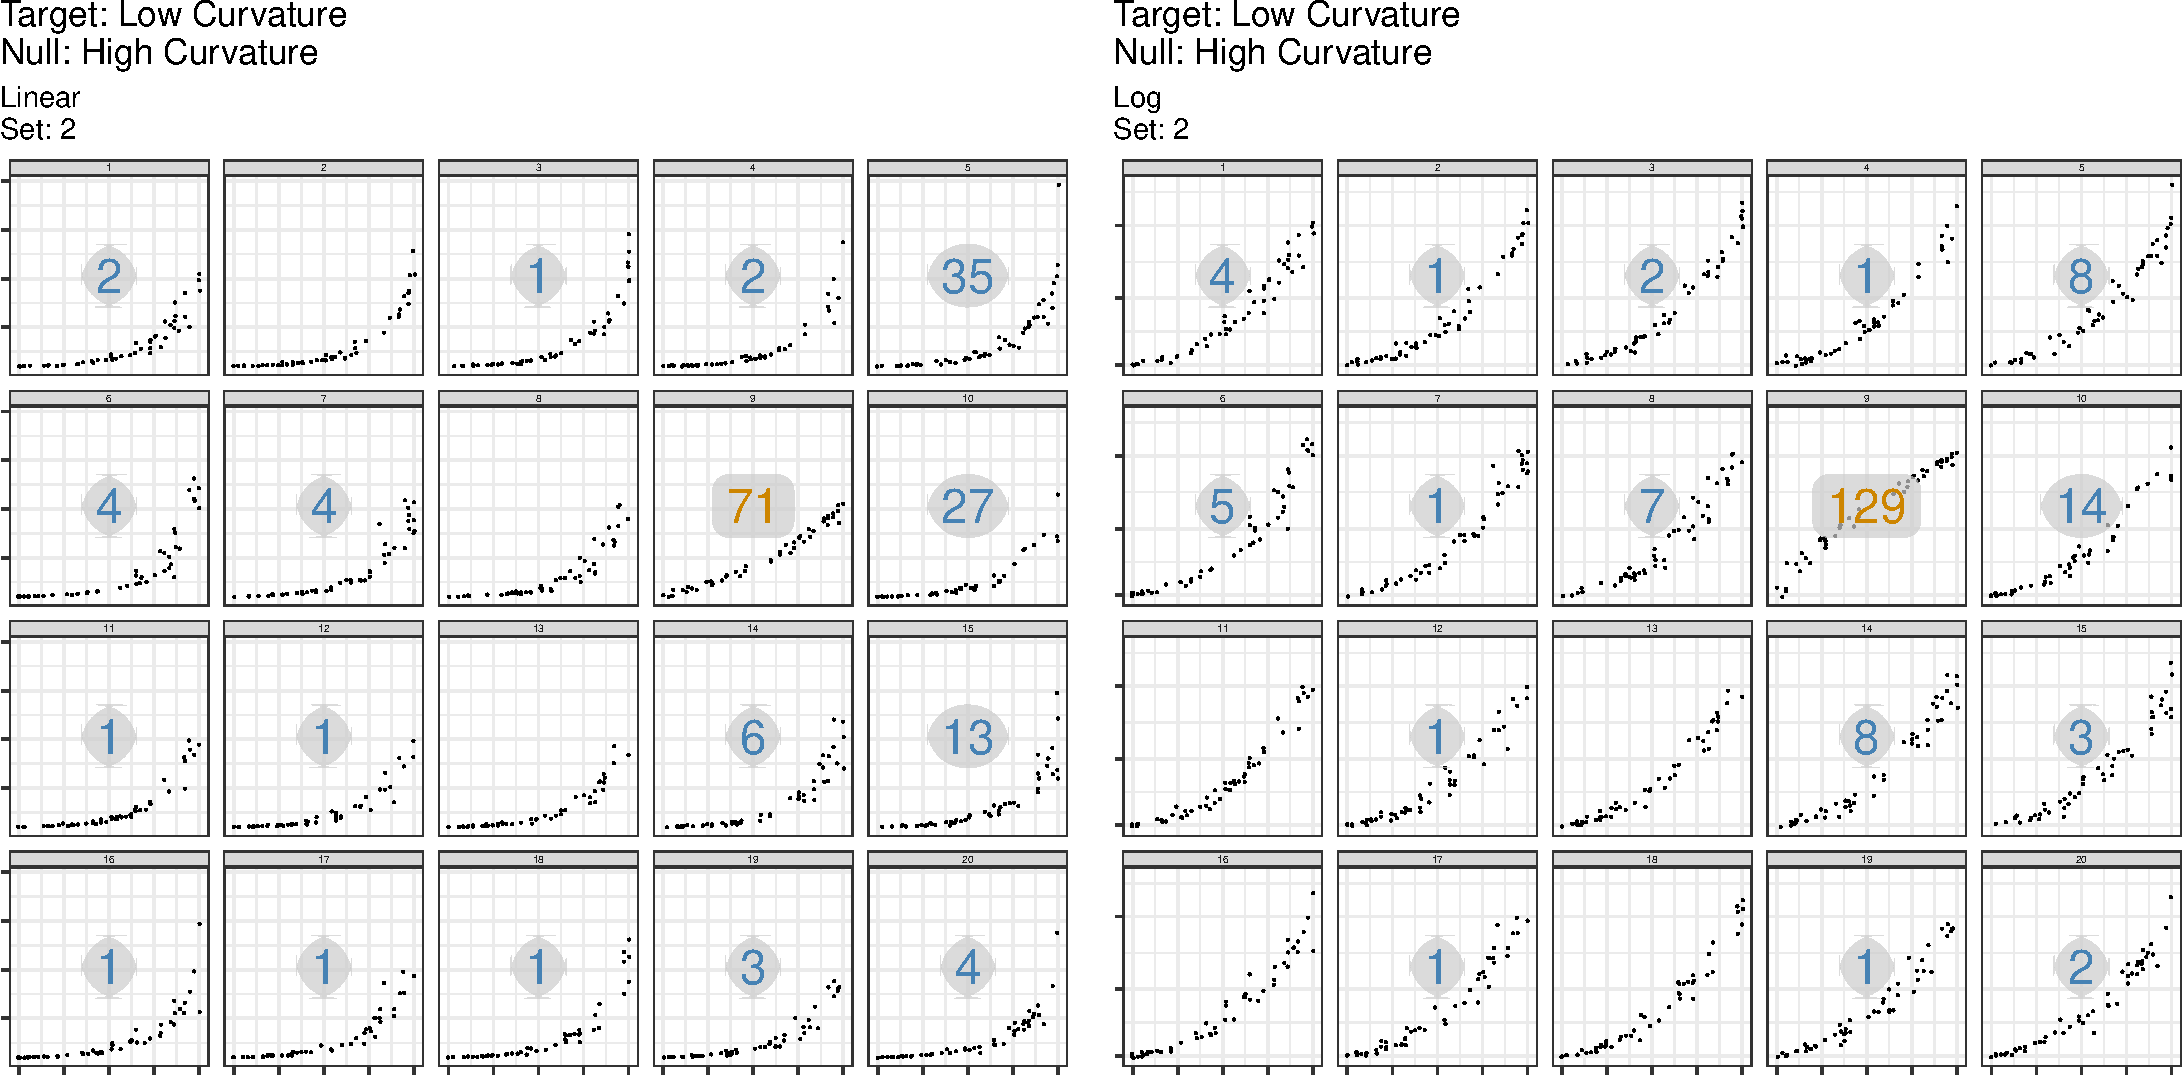
\includegraphics[width=\linewidth,]{appendix-3_files/figure-latex/unnamed-chunk-6-6} \end{center}

\newpage

\bibliographystyle{apalike}
\renewcommand\refname{References}
\bibliography{bibliography.bib}



\end{document}
